%%%%%%%%%%%%%%%%%%%%%%%%%%%%%%%%%%%%%%%%%%%%%%%%%%%%%%%%%%%%%%%%%%%%%%%%%%%%%%%%
% For the use of University of Amsterdam
% Master of AI thesis  --  ported from main-claude.tex into the new
% mscaithesis template (structure follows template.tex)
%%%%%%%%%%%%%%%%%%%%%%%%%%%%%%%%%%%%%%%%%%%%%%%%%%%%%%%%%%%%%%%%%%%%%%%%%%%%%%%%

% The class loads xcolor itself; pass the options the tables need up front.
\PassOptionsToPackage{table,dvipsnames}{xcolor}
\documentclass[openany]{mscaithesis}  % openany: no forced blank pages between chapters

\usepackage[utf8]{inputenc}
\usepackage[english]{babel}
\usepackage{graphicx}
\graphicspath{{./}{media/figures/}}
\usepackage{booktabs}
\usepackage{colortbl}
\usepackage{multirow}
\usepackage{makecell}
\usepackage{float}
\usepackage{microtype}
\setlength{\emergencystretch}{1.5em}
\usepackage{flushend}   % balance the two columns on the last page of each chapter
% Let floats fill pages more aggressively (avoids near-empty float pages)
\renewcommand{\topfraction}{0.9}
\renewcommand{\bottomfraction}{0.6}
\renewcommand{\textfraction}{0.05}
\renewcommand{\floatpagefraction}{0.8}
\renewcommand{\dbltopfraction}{0.95}
\renewcommand{\dblfloatpagefraction}{0.7}
\setcounter{topnumber}{4}
\setcounter{dbltopnumber}{4}
\setcounter{totalnumber}{6}

\usepackage{amssymb} % Math packages are (on purpose) not included in the class
\usepackage{amsfonts}
\usepackage{amsmath}
\usepackage{amsthm}

\usepackage{xurl}
\usepackage{tikz}
\usetikzlibrary{positioning,arrows.meta,fit,backgrounds}

% Template uses natbib + ACM-Reference-Format (a numeric style); the numbers
% option makes natbib accept it.
\usepackage[numbers]{natbib}

% ---- commands carried over from the old draft ----------------------------
\definecolor{rowhl}{RGB}{209, 231, 255}
\newcommand{\tbest}[1]{\cellcolor{rowhl}#1}  % table-wide best cell (per column)
\newcommand{\pmsd}[1]{{\scriptsize$\pm$#1}}  % mean$\pm$sd in tables (seed spread)
\setlength{\tabcolsep}{4pt}
\renewcommand{\arraystretch}{1.08}

\newcommand{\red}[1]{{\color{red}{#1}}}
\newcommand{\todo}[1]{{\color{orange}\textbf{[TODO: #1]}}}
\newcommand{\todome}[1]{{\color{magenta}\textbf{[TODO-PIOTR: #1]}}}

%%%%%%%%%%%%%%%%%%%%%%%%%%%%%%%%%%%%%%%%%%%%%%%%%%%%%%%%%%%%%%%%%%%%%%%%%%%%%%%%
% DOCUMENT METADATA
%%%%%%%%%%%%%%%%%%%%%%%%%%%%%%%%%%%%%%%%%%%%%%%%%%%%%%%%%%%%%%%%%%%%%%%%%%%%%%%%

\title{Two Regimes of Appearance Bias in Sign Language Recognition:\\
When Synthetic Counterfactuals Help and When They Don't}

% Date on which the thesis is submitted
\date{\red{2026/??/??}}

\author{Piotr \textsc{Sobecki}}
\studentnumber{15127206}
\period{\red{Period in which the research was carried out}}
\credits{36 ECTS}
\examiner{\red{Dr A. Person}}
\dailysupervisor{Casper Thuis}
\uvasupervisor{Dr James Trujillo}   % NOTE: verify role mapping
\addsupervisor{Angelos Nalmpantis}  % NOTE: class has no "second reader" slot

\begin{document}
\maketitle

\frontmatter
        \chapter*{Abstract}
                \begin{adjustwidth}{4cm}{4cm}
\todo{refine abstract at the end}
Sign language recognition (SLR) models struggle under test domain shift:
unseen signers and new recording conditions. Appearance-bias findings in action
recognition motivate asking whether SLR models key on incidental visual
properties of the recorded signers rather than the signing itself. This thesis asks
whether \emph{synthetic appearance counterfactuals} --- edited training
videos that change appearance while preserving the performed sign --- can
remove this bias. We first diagnose the problem: signer
identity is recoverable from every feature space we test, including
pose-based ones. We then intervene with two synthesis pipelines:
motion-locked avatar re-renders of a self-recorded Dutch Sign Language
(NGT) corpus, and generative per-frame appearance edits of ASL Citizen
videos. The outcome splits into two regimes.
In the low-diversity NGT setting (4 training signers, one studio
environment), synthetic signers more than double cross-signer retrieval (R@1 $0.23 \to 0.65$ test$\to$train;
$0.25 \to 0.70$ train$\to$test, 3 seeds). On the large, signer- and
environment-diverse ASL Citizen benchmark, the counterfactuals leave
recognition essentially unchanged across every objective family we try
--- an informative null: with 460 pretraining signers and 35 training
signers, appearance invariance is already bought by real diversity.
Synthetic counterfactuals earn their cost precisely where real signer
diversity is scarce --- and are largely redundant where it is not.
\end{adjustwidth}

\tableofcontents

\listoffigures

\listoftables

\chapter{List of Abbreviations}
        \begin{table}[h]
                \centering
                \begin{tabular}{cl}
                                ASL & American Sign Language \\
                                AUC & area under the ROC curve \\
                                CE & cross-entropy \\
                                CI & confidence interval \\
                                CLS & classification token \\
                                CSLR & continuous sign language recognition \\
                                DCG & discounted cumulative gain \\
                                FT & fine-tuned \\
                                InfoNCE & information noise-contrastive estimation \\
                                KL & Kullback--Leibler (divergence) \\
                                mocap & motion capture \\
                                MRR & mean reciprocal rank \\
                                NGT & Nederlandse Gebarentaal (Dutch Sign Language) \\
                                NGT775 & the unreleased 775-sentence NGT corpus used in this thesis \\
                                P@$k$ & precision at rank $k$ \\
                                R@$k$ & recall at rank $k$ \\
                                RGB & red--green--blue (raw video input) \\
                                SDDA & Signer Diversity-driven Data Augmentation \\
                                SLR & sign language recognition \\
                                SupCon & supervised contrastive (objective) \\
                                t-SNE & t-distributed stochastic neighbour embedding \\
                                VSSign & visually similar sign \\
                \end{tabular}
        \end{table}


\setlength{\parskip}{5pt}

\twocolumn
\mainmatter
        \chapter{Introduction}
Sign languages are the primary languages of Deaf communities, and they
are full natural languages rather than manual renderings of the
surrounding spoken language. The World Federation of the Deaf estimates
that more than 70 million deaf people belong to signing communities,
using over 200 national sign languages~\cite{wfd2026faq}.

Automatic processing of these languages has been studied extensively, and
recent surveys document an active literature spanning recognition,
translation and
generation~\cite{bragg2019sign, koller2020quantitative,
nunezmarcos2023survey, decoster2024machine}. Widely usable tools,
however, do not yet exist, and reported progress rests substantially on
having seen the signer before: recent translation systems lose most of
their accuracy when re-evaluated on signers unseen in
training~\cite{artiagaRethinkingSignLanguage2025}. Closing that gap needs
representations that generalise beyond the signers and recording
conditions any one corpus contains, which is the prerequisite this thesis
works on.

\emph{Sign language recognition} (SLR) maps video of signing to
linguistic units. It is conventionally split into \emph{isolated} SLR,
where a clip contains a single sign and the model predicts a \emph{gloss}
(a written label for a sign, by convention in capitals) from a fixed
vocabulary, and \emph{continuous} SLR, where a sentence-length recording
is transcribed as a gloss sequence; both are distinct from translation,
which targets spoken-language text. This thesis works at the isolated
level on one corpus and the sentence level on the other, evaluating both
by retrieval (\S\ref{sec:eval-protocols}).

SLR faces two distinct problems that this
thesis addresses together.
The first is \emph{data scarcity}, whose scale is easy to understate. The
largest sign language video corpus holds roughly $3{,}200$ hours, and
covers only about twenty-five of the more than three hundred sign
languages in use worldwide~\cite{tanzerYouTubeSL25}; a single speech
recognition model of the same period was trained on $680{,}000$ hours of
audio~\cite{radfordRobustSpeechRecognition2022}. Annotated data is
scarcer again: the largest corpora are weakly supervised harvests whose
text is scraped or machine-transcribed rather than
glossed~\cite{tanzerYouTubeSL25, liUniSignUnifiedSign2025}, and glossing
proper is slow expert work, about an hour per ninety seconds of video for
How2Sign~\cite{duarteHow2Sign2021}, with formats that are not
standardised across
corpora~\cite{desistoChallengesSignLanguage2022, DataProblem}. 

The second is \emph{appearance bias}: a video model can score well on a benchmark by
exploiting the static, incidental visual properties of whoever happened to
be recorded (clothing, skin tone, body shape, background) rather than focusing exclusively on
the motion that carries the linguistic content. In the action-recognition
literature this second phenomenon is well
documented~\cite{leiRevealingSingleFrame2023, ilicAppearanceFreeAction2022,
liMitigatingEvaluatingStatic2023a, zhangDontJudgeLook2024}; action
recognition is also the domain closest to ours (SLR inherits its video
backbones and training recipes from it), so we treat its bias findings
and interventions as directly relevant, and review them in
\S\ref{sec:related-appearance-bias}. The two
problems interact (fewer recorded signers make appearance shortcuts
easier to exploit), but they are separate, and this thesis uses one
mechanism against both: synthetically generated signing adds data where
data is scarce, and its controlled appearance variation attacks the bias
directly.

For sign language this is not an abstract concern. Signing is performed by
people, and the appearance dimensions a model may latch onto (skin tone,
gender, clothing, recording environment) correlate directly
with demographic groups~\cite{heldrethWhichSkinTone2024,
schumannConsensusSubjectivitySkin2023}. A sign language recognition system that implicitly
keys on appearance will degrade unpredictably for signers who look unlike its
training population. Signer variation itself is a long-standing focus of
SLR research, and signer-independent evaluation is an established
protocol (\S\ref{sec:related-signer-independent} reviews the remedies
proposed). Yet while appearance bias is actively studied in general
action recognition, it has received little direct attention in the sign
language domain.

The field's dominant response to signer variation has been indirect: move
from RGB input to pose-based input. Pose representations discard pixels
(and with them, most appearance information), and a visible trend in recent
benchmarks and challenges pushes towards signer-independent evaluation and
pose-based methods~\cite{jangSigningOutsideStudio2022,
luqmanSignEval2025Challenge2025a, jiangSignCLIPConnectingText2024}. The
SignEval 2025 challenge makes the trend explicit: in its signer-independent
recognition task, every submitted system was pose-based, by design,
since the organisers distributed only MediaPipe-derived pose features
extracted from the underlying (RGB-recorded) Isharah videos, citing signer
overfitting~\cite{luqmanSignEval2025Challenge2025a,
alyamiIsharahLargeScaleMultiScene2026b}: for that task, RGB-based
approaches were excluded from the outset rather than tried and outperformed.

But pose is not a free lunch. Pose extractors are themselves learned
RGB models, with demographic and mechanical failure modes of their own
(\S\ref{sec:related-work-modality}). Meanwhile recent self-supervised
RGB representations report stronger sign representations than pose-based
alternatives~\cite{wongSignRepEnhancingSelfSupervised2025}. If RGB has the higher ceiling, then abandoning it to escape
appearance bias trades accuracy for robustness. The alternative this thesis
explores is to keep RGB and attack the bias directly with \emph{synthetic
appearance counterfactuals}: renderings or edits of the same signing motion
under different appearances, so that appearance becomes a factor the model
can be explicitly trained, or shown, to ignore.

The approach we set out to build is the one that guarantees the
counterfactual property by construction: record signing with motion
capture, retarget the captured motion to synthetic avatars, and render
them. Every render then shows exactly the same signing motion under a
freely chosen appearance, so motion preservation is a property of the
pipeline rather than an assumption; we call these \emph{motion-locked
re-renders}. But this route cannot be
applied to an existing benchmark where videos are plain RGB with no
motion capture attached, so the only way to use it at benchmark scale would
be to record a new mocap corpus of comparable size.

We therefore approximate it. Modern generative image editors can rewrite
the appearance of an existing video frame by frame: we edit
real benchmark videos (changing clothing, adding glasses, altering skin
tone, swapping in a different signer) while leaving the rest of each
frame alone. This recovers the appearance-variation axis of the
re-renders at a cost that scales to existing benchmarks. It is an
approximation, not a substitute: the edits are per-frame appearance
rewrites, so the signing motion is preserved only insofar as the editor
leaves it untouched, not by construction.

\begin{figure*}[t]
\centering
\includegraphics[width=\textwidth]{method_overview.pdf}
\caption[Method overview: appearance counterfactuals in contrastive
training]{\textbf{Method overview.} Setting A is the high-diversity
regime, Setting B the low-diversity one. Objectives and loss weights are defined in
\S\ref{sec:method-objectives}.}
\label{fig:method_overview}
\end{figure*}

In this thesis we therefore study two dataset regimes that differ in
appearance diversity, both with signer-disjoint evaluation. The first is
a low-diversity setting in which motion capture is available: NGT744, a
small, self-recorded Dutch Sign Language (NGT) corpus recorded from four
signers in a single studio and evaluated in another, so that both signer
identity and capture conditions are near-constant during training. There
the motion-locked pipeline runs in full, and we compare the two
counterfactual routes head to head, avatar re-renders against generative
edits of the same videos, under matched conditions. The second is a
high-diversity setting in which only RGB video is available: ASL Citizen,
whose 35 training signers record themselves on their own webcams, so that
identity, lighting, framing and background all vary. There only the
generative route applies, and we ask whether synthetic appearance data
still helps. NGT744 is additionally low-resource in absolute size; ASL
Citizen is not large by general-vision standards, but it is diverse. The
two settings turn out to give different answers, and that contrast, where
synthetic appearance variation earns its cost and where it does not, is
the core result of the thesis.

This thesis asks whether appearance bias is measurable in modern sign
language representations, and whether synthetic appearance
counterfactuals can reduce it; Figure~\ref{fig:method_overview}
summarises how they enter training. Concretely:

\begin{description}
\item[RQ1 (Diagnosis).] Do sign language video representations, namely pose-based
  (MediaPipe), RGB transformer
  (Logos/MViTv2 \cite{ovodovLogosWellTemperedPretrain2025}), RGB CNN (I3D),
  and contrastively text-aligned (SignCLIP \cite{jiangSignCLIPConnectingText2024}),
  encode signer identity beyond sign content, and to what degree?

\item[RQ2 (Low-diversity regime).] Do synthetic appearance
  counterfactuals improve retrieval where training diversity is minimal
  (the NGT744 corpus, four signers in a single studio)? We ask this of
  each synthesis route on its own before comparing them:
  \begin{description}
  \item[RQ2a.] Do motion-locked re-renders (avatar renders driven by real
    motion capture) help when added as extra views under a supervised
    contrastive objective~\cite{khosla2020supervised}?
  \item[RQ2b.] Do generative appearance edits help in the same role?
  \item[RQ2c.] At matched strength, content and viewpoint, how do the two
    routes compare?
  \end{description}

\item[RQ3 (High-diversity regime).] In a high-diversity setting (ASL
  Citizen), do generative appearance edits
  (clothing, glasses, skin tone, signer swap), our
  scalable approximation of motion-locked synthesis, improve
  retrieval, either as counterfactual supervision when fine-tuning the backbone itself or as training data for a contrastive embedding head?

\item[RQ4 (Interpretation).] What do the RQ3 interventions do
  to the embedding space itself: where do the synthetic counterfactuals
  land relative to their source videos and to a genuine signer change
  (do they stay local, and do they occupy a separable ``synthetic'' region),
  and does any training objective actually reduce the signer identity
  encoded in the features, measured both by distance geometry and by
  linear decodability?
% Answerable by: \S\ref{sec:results-l2-raw} + \S\ref{sec:results-ft-probes}
% (distance ratio + linear decoding, incl. the dissociation, lines
% 1309-1380 and 2002-2108) and \S\ref{sec:results-aug-geometry}
% (displacement locality, sim-to-real separability, de-shift collapse,
% lines 2110-2323). "genuine signer change" echoes the n.disp calibration
% (lines 2141-2151); "separable synthetic region" echoes measurement 2
% (lines 2158-2174); "distance geometry ... linear decodability" echoes the
% two probes (lines 2008-2021).
\end{description}




        \chapter{Related Work}
This chapter follows the argument of the introduction. We begin with how
SLR has treated signer variation, as an evaluation protocol and as
something to suppress (\S\ref{sec:related-signer-independent}). We then
turn to appearance bias itself, which is well studied in action
recognition and barely touched in sign language, and to why the action
recognition remedies do not transfer
(\S\ref{sec:related-appearance-bias}). We then trace how benchmarks became
more diverse and what that did to modality preference
(\S\ref{sec:related-work-benchmarks}), examine the resulting move from RGB
to pose and what it costs (\S\ref{sec:related-work-modality}), and close
with synthetic data as the intervention family this thesis draws on
(\S\ref{sec:related-work-synthetic}).

\section{Signer-independent SLR}
\label{sec:related-signer-independent}
Signer variation is a long-standing generalisation axis in SLR, and the
field has responded on two fronts: evaluation protocols that withhold
signers, and methods that suppress signer information.

On the protocol side, signer-independent evaluation is well established.
The ChaLearn LAP challenge on AUTSL made large-scale signer-independent
isolated recognition a community benchmark (226 signs, 43 signers,
signer-disjoint splits); its winning entries relied heavily on pose
estimation, graph convolutions, and
ensembling~\cite{sincanChaLearnLAPSigner2021}. PHOENIX-2014 ships a
dedicated signer-independent split alongside its default protocol, used
by signer-invariant CSLR work~\cite{zuoImprovingContinuousSign2024},
and ASL Citizen is signer-disjoint by construction~\cite{aslcitizen}.
Recent challenges push the setting further: the Cross-View Isolated SLR
challenge adds camera viewpoint to the held-out axes~\cite{CV-ISLR},
and the SignEval 2025 challenge makes signer-independent CSLR on Isharah
a dedicated track, distributing only pose features extracted from the
RGB recordings out of concern for signer overfitting and
privacy~\cite{luqmanSignEval2025Challenge2025a,
alyamiIsharahLargeScaleMultiScene2026b}, a design choice we return to in
\S\ref{sec:related-work-modality}.

On the method side, three families recur. Adversarial approaches train
the encoder so that signer identity cannot be recovered from it:
Ferreira et al.\ apply signer-adversarial training to isolated
recognition~\cite{Ferreira2021}, and Zuo and Mak add a signer removal
module that disentangles signer statistics from the recognition features
of a CSLR model~\cite{zuoImprovingContinuousSign2024}. Disentanglement
approaches separate signer style from sign content explicitly, as in
contrastive disentangled meta-learning for signer-independent
translation~\cite{jinContrastiveDisentangledMetaLearning2021}. Data-side
approaches raise the signer diversity the model sees, with more real
signers or with synthetic signer variety such as SDDA's
diffusion-generated signers (\S\ref{sec:related-work-synthetic}).
Pose-centric modelling, finally, sidesteps the pixel appearance
altogether~\cite{kratimenosIndependentSignLanguage2020,
tranRegionAwarePoseModeling2025}, at the cost examined in
\S\ref{sec:related-work-modality}.

What these approaches share is that appearance is handled wholesale: held
out with the signer, removed adversarially, averaged over by adding
signers, or discarded along with the pixels. None isolates which visual
properties carry the signal, or tests whether changing exactly those,
with the signing held fixed, removes the shortcut.
\S\ref{sec:related-appearance-bias} takes up that question.
\section{Addressing appearance bias}
\label{sec:related-appearance-bias}
That action-recognition benchmarks reward static appearance cues is an
empirical finding rather than an assumption: RESOUND quantifies the
representation bias of action datasets and shows the standard ones are
skewed towards static objects, scenes and
people~\cite{liRESOUNDActionRecognition2018}. RESOUND both resamples
existing corpora to reduce that bias and collects Diving48, a
fine-grained benchmark designed to remove it. The effect is severe enough
that actions stay recognisable once the actor is gone: masking out
detected people in UCF101 still leaves a two-stream network at $53.1\%$,
against $84.3\%$ on the unmodified
videos~\cite{heHumanActionRecognition2016}.

Crucially for this thesis, the bias is a property of the training data
rather than of the architecture.
\citet{byvshevAre3DConvolutional2022a} measure how much temporal
structure a 3D convolutional network's filters retain and find it
collapsing with depth in Kinetics-trained models, then retrain the same
architectures on synthetic data in which motion and appearance are
decoupled by construction; there the collapse disappears, and they
conclude that the architecture is not inherently appearance-biased.
\citet{kowalQuantifyingLearningStatic2025} reach a compatible conclusion
with a representation-level probe, pairing restyled videos (dynamics
fixed, appearance changed) against frame-shuffled ones (appearance fixed,
dynamics destroyed) to score how static each channel is, and find most
models static-biased. If the bias is inherited from data, it can be
attacked by reshaping data.

Remedies fall into two families. The first restructures the training
signal so that positives share motion while appearance varies. Motion
Coherent Augmentation permutes a clip's RGB channels and blends the
result back into the original, a cheap hue shift that leaves saturation
and value untouched, and pairs it with a loss aligning the augmented
clip's prediction to the original clip's rather than to the
label~\cite{zhangDontJudgeLook2024}. Tubelet-contrastive self-supervision
goes further, building positive pairs that share only local motion by
pasting synthetic moving tubelets into different videos, so that
appearance cannot solve the pretext
task~\cite{thokerTubeletContrastiveSelfSupervisionVideoEfficient2023b}.
The second family suppresses the static signal directly. StillMix uses a
2D network to flag frames from which the action is already predictable,
then tiles such a frame into a motionless clip and blends it into
training video~\cite{liMitigatingEvaluatingStatic2023a}; ALBAR repeats a
single frame into a motionless clip, passes it through the same encoder
as the real clip, and penalises any confident prediction from it with a
negative cross-entropy and an entropy
term~\cite{fioresiALBARAdversarialLearning2025}; SMAD combines
multi-aspect adversarial training with spatial actionness
reweighting~\cite{duanMitigatingRepresentationBias2023}; and
\citet{rastegarBackgroundNoMore2024} treat the background as a confounder
and intervene causally at both training and test time.

Two of these lines already reach past the background to the actor:
StillMix demonstrates that the foreground is itself a source of static
bias, and ALBAR names clothing, skin colour and facial hair explicitly.
Their mechanism, however, is to \emph{suppress} the static channel, by
masking it, blending a motionless clip into it, or penalising confident
predictions made from it. That is not available in signing, where the
same channel carries linguistic content: facial expression, mouthing and
fine handshape are part of what the label depends on. The intervention
must therefore change appearance while preserving motion, rather than
removing appearance information, which is what makes a counterfactual
rather than a suppression the natural instrument here.

Within sign language, the nearest work targets demographic disparity and
research practice rather than the appearance content of the training
distribution. Atwell et al.\ study and mitigate demographic bias on ASL
Citizen, reducing performance disparities without a loss of
accuracy~\cite{atwellStudyingMitigatingBiases2024}, and a Deaf-led review
documents systemic biases in how sign language AI research selects
datasets, labels and modelling
assumptions~\cite{desaiSystemicBiasesSign2024}.
SignRep~\cite{wongSignRepEnhancingSelfSupervised2025} intervenes on the
representation instead, suppressing appearance with an adversarial style
loss during self-supervised pretraining
(\S\ref{sec:related-work-modality}). The closest data-side intervention
is SDDA~\cite{fuSignerDiversitydrivenData2024b}, treated with the other
synthetic-data work in \S\ref{sec:related-work-synthetic}.

Editing the appearance of sign video has precedent, with a different
goal: diffusion-based editing has been used to \emph{anonymise} sign
video, changing signer appearance while preserving linguistic
content~\cite{xiaDiffusionModelsSign2024}, and pose-based appearance
transfer re-renders one signer's motion under another's appearance in
skeleton space~\cite{moryossefPoseBasedSignLanguage2025}. This thesis
repurposes that edit family as training-time counterfactuals, in pixel
space so that the RGB modality the rest of the pipeline consumes is
retained, and asks what the edits buy the recogniser rather than the
privacy of the signer. It differs from SDDA in pairing generative edits
with motion-locked re-renders, in asking what the intervention does to
the embedding space rather than only to task accuracy, and in testing
both across two diversity regimes.
% Framing note (2026-07-11, applied 2026-07-28): the qualification of story
% point 1 ("not well-tackled in the SL domain" rather than "unexplored")
% acknowledges Atwell/Desai/SDDA while keeping the novelty claim narrow and
% true; aligned with the SDDA scoping in the intro (pivot paragraph) and the
% Synthetic data section.

\section{Benchmarks and the diversity axis}
\label{sec:related-work-benchmarks}
As surveyed by \citet{kalinowskiMachineLearningSign2026}, a large share of
sign language recognition research has been conducted on two
studio-recorded benchmarks, Phoenix2014~\cite{kollerContinuousSignLanguage2015}
(extended to Phoenix2014T for the SLT task~\cite{camgozNeuralSignLanguage2018})
and CSL-Daily~\cite{CSL-daily}. These corpora hold recording conditions
almost constant, and on them RGB architectures were competitive
(\S\ref{sec:related-work-modality}). Their homogeneity is also their
documented weakness: \citet{jangSigningOutsideStudio2022} note the lack of
variance in setting and background, and \citet{CE-CNSL} identify the
studio setting as a bottleneck and release CE-CNSL to address it. More
recently, \citet{alyamiIsharahLargeScaleMultiScene2026b} target both the
lack of diversity and signer-independent evaluation, and their Isharah
dataset supplies the CSLR track of the SignEval 2025
Challenge~\cite{luqmanSignEval2025Challenge2025a}. As benchmarks grew more
varied, the field's preference shifted towards pose input, whose
appearance invariance is most valuable exactly where appearance varies
most.

ASL Citizen~\cite{aslcitizen} belongs to this harder lineage: it is
signer-disjoint by construction and, unlike a single-studio corpus,
aggregates recordings made by participants on their own webcams, so
lighting, framing and background vary along with the signer. It also
ships per-participant demographic metadata, which makes the composition
of its signer population inspectable rather than
assumed~\cite{atwellStudyingMitigatingBiases2024}. We adopt it as the
high-diversity setting of this thesis, and NGT744, recorded from four
signers in one studio, as the low-diversity setting: the two mark
opposite ends of the axis this thesis is about, while both evaluate
signer-independently.

\section{Input modality}
\label{sec:related-work-modality}
That shift has a clear empirical basis. On the studio benchmarks, RGB CNN
architectures such as
SlowFastSign~\cite{ahnSlowFastNetworkContinuous2023} achieved strong
performance; on the more varied ones, pose-based representations show
improved robustness at competitive
accuracy~\cite{minCloserLookSkeletonbased2025}, a trend usually
attributed to the inherent
invariance of pose representations to appearance factors such as clothing,
background, and
lighting~\cite{moryossefEvaluatingImmediateApplicability2021,
kratimenosIndependentSignLanguage2020, tranRegionAwarePoseModeling2025}.
Pose-based models, however, discard substantial
visual information present in the original RGB signal, raising the question
of whether the improved robustness of pose-based approaches stems solely
from appearance invariance, or whether RGB-based models simply fail to
capture motion cues in the presence of strong appearance signals.

The robustness attributed to pose input is also bounded by the extractor
that produces it, which is itself a learned RGB model. The standard
training and evaluation sets for pose estimation under-represent
darker-skinned individuals~\cite{lachanceCaseStudyFairness2023,
hasanHi5SyntheticData2024}, the few existing fairness audits of pose
estimators reach conclusions that flip with the choice of evaluation
set~\cite{lachanceCaseStudyFairness2023, xiangFairHumanCentricImage2025},
and on ASL Citizen the pose-based baseline shows larger skin-tone and
gender performance disparities than its RGB
counterpart~\cite{atwellStudyingMitigatingBiases2024}. There are
mechanical failure modes too: MediaPipe Holistic's hand
region-of-interest prediction breaks down on non-ideal hand
orientations~\cite{moryossefOptimizingHandRegion2024}, and both OpenPose
and MediaPipe degrade precisely where hands interact with each other or
the face, interactions that are linguistically load-bearing in
signing~\cite{moryossefEvaluatingImmediateApplicability2021}. In our own
extraction MediaPipe produced no usable feature file for $8\%$ of ASL
Citizen training videos (Table~\ref{tab:raw_feature_l2_probe}).

The appearance bias of RGB models is, however, a property of their
training data rather than of the modality itself
(\S\ref{sec:related-appearance-bias}); the same evidence shows it
survives the move to transformer backbones, which
\citet{liMitigatingEvaluatingStatic2023a} mitigate with augmentation on a
video Swin transformer. That is the question we ask of the transformer
backbones now common in SLR.

\subsection{Single-stream scope}
A natural alternative is
to combine RGB and pose in hybrid architectures, e.g.\ a two-stream
network~\cite{chenTwoStreamNetworkSign}; we do not pursue this, preferring a
single-stream RGB approach for its lower inference cost and simpler
pipeline, considerations that real-time sign language processing makes
explicit~\cite{moryossefRealTimeMultilingualSign2024}. Throughout this thesis we therefore consider \emph{single-stream}
methods only: every backbone we train, probe, or compare consumes one input
stream (RGB video or pose), and multi-stream or hybrid architectures are
out of scope on compute and inference-cost grounds.

\section{Synthetic data}
\label{sec:related-work-synthetic}
If appearance bias is inherited from training-data statistics
(\S\ref{sec:related-appearance-bias}), reshaping the training
distribution is a way to reduce it. Sign language recognition, however, lacks a counterpart
to the large, temporally rich pretraining corpora available in general video
understanding, motivating the use of \emph{synthetic} data to reshape the
training distribution directly. Knapp and Bohacek~\cite{knapp2025synthetic}
generate synthetic action video via controllable 3D Gaussian avatar pose
transfer and show gains when used as augmentation; related work renders
synthetic action data in GTA V~\cite{guoLearningVideoRepresentations2022} and
studies synthetic data for temporal alignment~\cite{SVLTA_Du_2025}. Li et
al.\ show that data generated by a text-to-video diffusion transformer can
benefit data-limited action
understanding~\cite{liRoleVideoGeneration2025}, but do not consider sign
language; Knapp and Bohacek further note that sign-language tasks are among
those that have so far been unable to exploit the full potential of
synthetic video, as generated human motion suffers from uncanny
artefacts~\cite{knapp2025synthetic}; this thesis addresses that gap.

In general vision, generative augmentation is itself an established
line: DA-Fusion edits real training images with a diffusion model and
improves few-shot classification, while cautioning that the gains are
task- and regime-dependent~\cite{trabuccoEffectiveDataAugmentation2024},
a caveat our two-regime result echoes in the sign domain.

\subsection{Sign language data augmentation approaches}
Walsh et al.\ show that sign language production can generate useful
synthetic augmentations for sign language translation, with a revealing
modality split: skeleton-level sign-stitching augmentation yields large,
consistent gains (at least 15\% across all reported metrics), whereas
photo-realistic RGB augmentation, via a GAN-based renderer (SignGAN) and
a Gaussian-splatting renderer
(SignSplat~\cite{ivashechkinSignSplatRenderingSign2025}), yields smaller
and mixed improvements, with GAN artefacts sometimes degrading
performance~\cite{walshUsingSignLanguage2025}. Diffusion-based sign
production continues this photo-realistic generation
line~\cite{SignDiff}.
% Verified against the paper (2026-07-11): pose-vs-RGB contrast confirmed,
% but the RGB methods compared are SignGAN + SignSplat — NOT diffusion.
% Story point 8 says "(Gaussian splatting, diffusion) don't work as well";
% the "diffusion" attribution is not supported by Walsh et al. — flagged
% to Piotr in the chat summary rather than silently corrected in his story.

Fu et al.'s Signer Diversity-driven Data Augmentation (SDDA) combines
diffusion-generated signer variation with a contrastive/adversarial
consistency objective and reports gains on
Phoenix2014T \cite{fuSignerDiversitydrivenData2024b}; the authors note that
their synthesized signers do not closely resemble real footage and frame
this as a limitation. We use the same consistency-objective family as one of
our backbone-fine-tuning ablations (\S\ref{sec:method-objectives}) and
return to the comparison in our Discussion (\S\ref{sec:discussion-regimes}):
SDDA's positive result is on a studio-recorded, lower-signer-diversity
corpus, closer to our low-diversity NGT744 regime than to our high-diversity ASL Citizen
regime, which we argue explains why the same idea saturates in one setting
and helps in the other.

~\citet{pengSyntheticViewAugmentation2025a} propose synthetic view augmentation using SMPL-X reconstruction
to address viewpoint generalisation, introducing new backgrounds and
viewpoints but not new signer
appearance; notably, their
synthetic viewpoints enter training only through the projected-keypoint
(pose) and rendered-depth streams of a multi-modal model, with view
augmentation of the RGB stream explicitly left to future work, whereas
this thesis targets the lack of variety in signer appearance directly, in
the RGB modality.

\subsection{Avatar and Unreal Engine approaches}
The closest precedent for our motion-locked route is Ranum's thesis on
synthetic avatar data for Dutch Sign Language
(NGT)~\cite{ranum3DAwarenessGeometry2024}. Like us, Ranum renders
synthetic avatars driven by recorded motion capture; unlike us, the
renders are evaluated in the pose modality, by extracting keypoints from
the rendered videos and training on those. In that modality the
synthetic data benefits recognition, but the thesis expects the gain to
transfer less well to the video modality, given the cartoon-like
appearance of the avatars used. Our experiments test exactly that
video-modality case: the renders enter training as RGB clips, appearance
included. 

Prior work has built gesture-producing virtual avatar systems using Unreal
Engine and motion capture~\cite{messinaModularSignLanguage2025}, and has
used Unreal-rendered virtual agents, animated from mocap and varied in
skin tone, lighting, background, and camera angle, as a scalable source
of training data for gesture recognition~\cite{loyVirtualAgentsScalable}.

What our work adds to this line is the counterfactual construction and
its controlled evaluation. Prior avatar pipelines generate synthetic
gesture or sign data at scale; none of them, to our knowledge, renders
the same captured signing under systematically varied appearance and
then asks, against matched real controls, what that variation buys. We
evaluate the renders directly as RGB training views for sign language,
compare them at matched view count against a real multiview control and
against generative edits of the same videos, and trace the effect into
the learned embedding space rather than reporting task accuracy alone.

        \chapter{Method}
\label{chap:method}
\todo{Add a method overview figure} This chapter presents the methodological contribution of the thesis: a
formal framing of signer appearance as an intervenable nuisance factor
(\S\ref{sec:method-notation}), a taxonomy of appearance counterfactuals
together with two synthesis routes that realise them
(\S\ref{sec:method-diffusion}), and training objectives that consume the
counterfactuals either as additional data or as explicit positives
(\S\ref{sec:method-objectives}). The concrete instantiation --- datasets,
backbones, training configurations, and evaluation protocols --- is
collected in Chapter~\ref{chap:setup}.

\section{Problem formulation}
\label{sec:method-notation}
% Formal notation block (2026-08-03): set/space definitions + typed maps in
% the register of Nalmpantis §4.1-4.2 (run-in headers, one object per
% paragraph, numbered display equations), grounded in this thesis's own task.
This section fixes the notation used throughout the chapter: the data we
train on, the encoder under study, the appearance-counterfactual operator
that both synthesis routes instantiate, and the retrieval task on which
every model is evaluated. The losses that bind these objects together are
formalised in \S\ref{sec:method-losses} and the evaluation protocols in
\S\ref{sec:eval-protocols}; here we define only the objects they operate
on.

\paragraph{Videos and labels.}
Let $\mathcal{X}$ denote the space of signing videos. A training corpus is
a finite set of annotated clips
\begin{equation}
\label{eq:dataset}
\mathcal{D} \;=\; \bigl\{(x_i,\, y_i,\, s_i)\bigr\}_{i=1}^{n}
\;\subset\; \mathcal{X} \times \mathcal{Y} \times \mathcal{S},
\end{equation}
where $y_i \in \mathcal{Y}$ is the linguistic label of the video $x_i$ and
$s_i \in \mathcal{S}$ identifies its signer; when convenient we write
$y(x)$ and $s(x)$ for the label and signer of a clip. The label space
$\mathcal{Y}$ differs between our two supervision regimes. On the isolated,
gloss-labelled benchmarks each video clip shows a single sign and
$\mathcal{Y} = \mathcal{G}$, a gloss vocabulary of $C = |\mathcal{G}|$
classes shared across signers. The continuous corpus supplies no gloss
vocabulary: full sentences are the unit of recording, and $\mathcal{Y}$ is
the set of recorded sentence identities. Throughout, the signer is a
nuisance variable: labels in $\mathcal{Y}$ are defined by what is signed,
never by who signs it, and the retrieval tasks of this thesis ask the
representation to match clips across $\mathcal{S}$ at fixed
$\mathcal{Y}$-label.

\paragraph{Encoder.}
Every training setting, whatever its objective, produces a single video
encoder
\begin{equation}
\label{eq:encoder}
f_\theta : \mathcal{X} \to \mathbb{R}^{d},
\qquad z \;=\; f_\theta(x),
\end{equation}
mapping a video clip to one embedding vector, where $\theta$ collects the
trainable parameters --- a video--text head over frozen backbone features,
the fine-tuned backbone itself, or the view-contrastive encoder; the
instantiations, and the dimension $d$ each uses, are given in
\S\ref{sec:setup-training}. Whether $z$ is $\ell_2$-normalised is a
property of the objective and is stated with each loss. After training,
$\theta$ is frozen and every analysis in this thesis --- retrieval,
probing, feature geometry --- operates on the embeddings $z$ alone.

\paragraph{Appearance counterfactual operator.}
The interventions of this thesis are appearance edits: maps
\begin{equation}
\label{eq:cf-operator}
T_a : \mathcal{X} \to \mathcal{X}, \qquad a \in \mathcal{A},
\end{equation}
where $\mathcal{A}$ indexes the available edit types and $T_a(x)$ shows
the signing of $x$ under a changed appearance. The defining intent is that
$T_a$ moves a video clip across the nuisance factor while leaving the linguistic
content intact,
\begin{equation}
\label{eq:motion-preservation}
y\bigl(T_a(x)\bigr) \;=\; y(x) \qquad \text{for all } a \in \mathcal{A},
\end{equation}
while the appearance --- and, for identity-changing edits, the apparent
signer --- differs. Whether Eq.~\eqref{eq:motion-preservation} actually
holds is a property of the synthesis route, not an assumption we grant
ourselves: the mocap-driven avatar renders satisfy it by construction,
because every render is driven by the same captured motion, whereas the
frame-wise diffusion edits satisfy it only insofar as the editor leaves the
motion untouched, an empirical matter we return to when interpreting
results. For the diffusion route, $\mathcal{A}$ is
the four-type edit taxonomy $\{\text{shirt},\, \text{glasses},\,
\text{skin tone},\, \text{signer swap}\}$; for the avatar route,
$\mathcal{A}$ ranges over avatar--viewpoint pairs
(\S\ref{sec:setup-generation}).

\paragraph{Positive sets.}
For a training video clip $x$ we write
\begin{equation}
\label{eq:cf-set}
\mathcal{T}(x) \;=\; \{x\} \,\cup\,
\bigl\{\, T_a(x) \;:\; a \in \mathcal{A}(x) \,\bigr\}
\end{equation}
for its counterfactual set, where $\mathcal{A}(x) \subseteq \mathcal{A}$
are the edits realised for $x$ (not every edit is generated for every
clip). The contrastive objectives of \S\ref{sec:method-losses} are built
on positive sets over a batch: for an anchor $u$ in a batch indexed by
$\mathcal{B}$,
\begin{equation}
\label{eq:positive-set}
P(u) \;=\; \bigl\{\, p \in \mathcal{B} \setminus \{u\}
\;:\; p \sim u \,\bigr\},
\end{equation}
where $\sim$ is the positive-defining equivalence of the run: membership
of one counterfactual set $\mathcal{T}(x)$ (an original and its edits;
counterfactual-contrastive), a shared gloss in $\mathcal{G}$ (gloss-level
contrast across signers), or a shared recording identity (the view-contrastive setting,
where all $K$ views of one recording --- real cameras and synthetic
renders alike --- are positives). Everything in the batch outside $P(u)$
acts as a negative.

\paragraph{Cross-signer retrieval.}
The task is retrieval with the frozen encoder. An evaluation protocol
supplies a query set $\mathcal{Q}$ and a reference gallery $\mathcal{R}$,
each element carrying a label in $\mathcal{Y}$; for a query $q$ the
gallery is ranked by decreasing cosine similarity
$\cos\bigl(f_\theta(q),\, f_\theta(r)\bigr)$, and retrieval at rank $k$
succeeds if a correctly labelled reference appears among the $k$
highest-ranked items:
\begin{equation}
\label{eq:recall-at-k}
\mathrm{R}@k \;=\; \frac{1}{|\mathcal{Q}|} \sum_{q \in \mathcal{Q}}
\mathbf{1}\Bigl[\, y(q) \in \bigl\{\, y(r) : r \in \mathcal{R}_k(q)
\bigr\} \Bigr],
\end{equation}
where $\mathcal{R}_k(q) \subseteq \mathcal{R}$ are the $k$ gallery items
most similar to $q$. The protocols of \S\ref{sec:eval-protocols}
instantiate $\mathcal{Q}$ and $\mathcal{R}$ per corpus --- including a
video-to-text variant in which the gallery holds text prototypes rather
than videos --- and share one structural property: evaluation signers are
unseen during training, and in the continuous-corpus protocol query and
gallery are
additionally produced by disjoint signers, making the retrieval itself
cross-signer.

\section{Synthetic appearance counterfactuals}
\label{sec:method-diffusion}


\subsection{Diffusion-based appearance editing}
We generate appearance counterfactuals for the isolated-benchmark corpus
by editing real training videos frame-by-frame with an open image
diffusion model; the model, compute, and the statistics of the edited
subset are given in \S\ref{sec:setup-generation}. Rather than
augmenting a uniform sample, targets are chosen worst-first
at the class level: every gloss is ranked by its number of distinct training
signers (ascending), with ties broken by a difficulty proxy --- per-class
nearest-centroid gloss accuracy computed on the from-scratch contrastive
baseline's test embeddings, a clustering measure that degrades precisely when
embeddings organise by signer rather than by sign --- and entire classes are
taken in rank order until the budget fills.
\todome{REWRITE PROPOSAL (03.08): the opener above binds the diffusion
route to ``the isolated-benchmark corpus'', but Setup and Results apply
Flux to NGT too (stride-4 NGT edits in \S\ref{sec:setup-generation}; the
single-view ladder arms E4/E6/E7/E10 are Flux-on-NGT) --- the binding is
false and it also makes the route-vs-corpus framing in the abstract too
clean. Proposed replacement for the first sentence: ``The first route
edits real training videos frame-by-frame with an open image diffusion
model; it requires nothing beyond the RGB video itself, so it applies to
any corpus. The model, compute, and edited-subset statistics are given in
\S\ref{sec:setup-generation}.'' Let Setup alone say which route ran
where. Same issue in the avatar subsection below.}
We propose a taxonomy of four independent appearance edit types
(Fig.~\ref{fig:aug_examples}); for each
selected source video we generate up to four edits, applied frame-by-frame:
\emph{shirt} (a clothing swap, the lowest-risk edit --- the video backbone's own training
augmentations already include colour jitter, so this edit's marginal value
over standard colour augmentation is itself an open question), \emph{glasses}
(addition/removal, with some risk of altering facial expression near the
eyes), \emph{skin tone} (the highest-risk edit for hallucination, e.g.\
occasional extra or malformed hand shapes), and \emph{signer swap} (a full
identity change, carrying the highest potential benefit for a
signer-independent task alongside the highest hallucination risk).

\subsection{Motion-preserving avatar counterfactuals}
For the continuous corpus we propose a second, motion-capture-driven
route: the captured 3D motion of a real signer is retargeted onto
synthetic avatars and re-rendered under multiple camera viewpoints
(\S\ref{sec:setup-generation}). Because this route starts from
ground-truth motion rather than a 2D image edit, the signing motion is
preserved by construction, and the route can vary camera viewpoint as
well as appearance --- an axis a 2D edit cannot reach from a single
input view.
\todome{REWRITE PROPOSAL (03.08), same corpus-binding issue as above:
``For the continuous corpus'' ties the avatar route to NGT by
definition. Propose opening with ``The second route is
motion-capture-driven: ...'' (rest verbatim) and closing with ``Unlike
the diffusion route it requires motion-capture recordings, so it applies
only where capture is controlled.''}

\section{Counterfactual-aware training objectives}
\label{sec:method-objectives}
We train encoders with these counterfactuals in three settings ---
two on an isolated, gloss-labelled benchmark and one on a continuous
corpus without a gloss vocabulary; their concrete configurations
(datasets, backbones, dimensions) are given in
\S\ref{sec:setup-training}. In every setting the counterfactuals enter
the objective either as additional labelled data or as explicit
positives matched to their source video; the loss formulations below
cover both mechanisms.

\subsection{Loss formulations}
\label{sec:method-losses}
Three distinct model components are trained in this thesis, and each has
its own objective; Table~\ref{tab:objective_map} maps components to
objectives before the formulations are given. The \emph{video--text
head} trains only its own parameters on top of frozen backbone features
--- the backbone receives no gradient. The \emph{backbone fine-tuning}
runs do the opposite: they update the video backbone itself, with a
disposable linear gloss head on top. The \emph{view-contrastive encoder}
of the continuous corpus again trains only its own parameters over
frozen backbone features, and has no text tower at all.

\begin{table*}[t]
\centering
\footnotesize
\setlength{\tabcolsep}{4pt}
\begin{tabular}{llll}
\toprule
\textbf{Component} & \textbf{What is trained} & \textbf{Objective} &
\textbf{Counterfactuals enter as} \\
\midrule
\makecell[tl]{Video--text head\\\scriptsize (SignCLIP, both towers,\\\scriptsize on frozen Logos/I3D/pose feats)} & \makecell[tl]{head only;\\input features frozen} &
\makecell[tl]{video--text InfoNCE,\\Eq.~\eqref{eq:nce}} &
\makecell[tl]{extra $(v,t)$ pairs (aug-as-data), or\\pair-SupCon
positives, Eq.~\eqref{eq:supcon}} \\
\addlinespace
\makecell[tl]{Backbone fine-tuning\\\scriptsize (Logos MViTv2-S)} & \makecell[tl]{the backbone itself\\($+$ linear
gloss head)} & \makecell[tl]{master loss, Eq.~\eqref{eq:master}:\\CE $+$
one invariance option} & \makecell[tl]{extra labelled clips and/or\\
invariance-term positives} \\
\addlinespace
\makecell[tl]{View-contrastive encoder\\\scriptsize (SignCLIP video tower only,\\\scriptsize on frozen Logos feats)} & \makecell[tl]{encoder only;\\backbone frozen}
& \makecell[tl]{SupCon over views, Eq.~\eqref{eq:supcon};\\video-only
InfoNCE at $K{=}1$} & \makecell[tl]{synthetic views as\\additional
positives} \\
\bottomrule
\end{tabular}
\caption{Which objective trains which component. The SupCon form of
Eq.~\eqref{eq:supcon} is shared by two components; what differs is the
positive-defining equivalence of Eq.~\eqref{eq:positive-set} ---
counterfactual instance for the head and backbone runs,
recording identity for the view-contrastive encoder.}
\label{tab:objective_map}
\end{table*}

\paragraph{Video--text head objective.}
The video--text head is trained with the symmetric InfoNCE
loss~\cite{oordRepresentationLearningContrastive2018}
we take from VideoCLIP~\cite{xuVideoCLIPContrastivePretraining2021}, over frozen
768-d backbone features; only the head's parameters receive gradients.
For a batch of paired video and text
embeddings $(v_i, t_i)$,
\begin{equation}
\label{eq:nce}
\begin{split}
\mathcal{L}_{\mathrm{NCE}} \;=\;
-\frac{1}{N}\sum_{i=1}^{N}\Bigl[&
\log \frac{\exp(v_i \cdot t_i)}{\sum_{j}\exp(v_i \cdot t_j)}\\
&+ \log \frac{\exp(v_i \cdot t_i)}{\sum_{j}\exp(v_j \cdot t_i)}
\Bigr],
\end{split}
\end{equation}
where the text side is the gloss rendered as a caption; following
VideoCLIP, the embeddings are not $\ell_2$-normalised and no temperature is
applied. Synthetic counterfactuals enter in one of two ways: as additional
$(v, t)$ pairs carrying their source video's gloss (aug-as-data), or --- in
the pair-SupCon configurations --- by replacing the video--text loss with
the supervised-contrastive form of Eq.~\eqref{eq:supcon} below, computed
over video embeddings alone with an original and its edits sharing one
instance label (counterfactual-contrastive). 

\paragraph{Backbone fine-tuning objectives.}
All fine-tuning objectives operate on the same representation: the
encoder embedding $z = f_\theta(x)$ of \S\ref{sec:method-notation},
instantiated as the 768-d CLS token the video backbone produces for a
32-frame clip $x$, which is also exactly the feature later re-extracted for
evaluation. A linear head $h$ maps $z$ to logits over the $C=|\mathcal{G}|$ glosses
of the training vocabulary. Every run minimises a total loss of the form
\begin{equation}
\label{eq:master}
\mathcal{L} \;=\; \mathcal{L}_{\mathrm{CE}}
\;+\; \lambda_{\mathrm{cons}}\, \mathcal{L}_{\mathrm{cons}}
\;+\; \lambda_{\mathrm{sup}}\, \mathcal{L}_{\mathrm{sup}}^{\mathrm{gloss}},
\end{equation}
where $\mathcal{L}_{\mathrm{cons}}$ stands for the run's
appearance-invariance term (the cosine pull below, the CLS-level contrast
that replaces it, or the pair of SDDA terms with their own weights),
$\mathcal{L}_{\mathrm{sup}}^{\mathrm{gloss}}$ for the optional gloss-level
contrastive auxiliary, and the runs differ only in which weights are
non-zero and in what the invariance term treats as positives. The four
paragraphs that follow define these ingredients; they belong to the
backbone fine-tuning runs only, not to the video--text head.

\paragraph{Cross-entropy (all backbone fine-tuning runs).}
Standard softmax cross-entropy $\mathcal{L}_{\mathrm{CE}} =
-\log p_{h(z)}(y)$ against the gloss label $y$. In paired runs the
augmented copies are classified too, carrying their source video's label
(augmentation-as-data), so CE is averaged over the $B$ originals and $M$
augmentations jointly.

\paragraph{Appearance-consistency pull (invariance option 1).}
For each original $z_i$ and each of its appearance-augmented copies
$z_i^{a} = f_\theta(T_a(x_i))$, $a \in \mathcal{A}(x_i)$, present in the batch, a
positive-only cosine pull with no negatives:
\begin{equation}
\mathcal{L}_{\mathrm{cons}} \;=\;
\frac{1}{|\mathcal{P}|}\sum_{(i,a)\in\mathcal{P}}
\bigl(1 - \cos(z_i,\, z_i^{a})\bigr),
\end{equation}
weighted by $\lambda_{\mathrm{cons}}=0.5$. This directly asks the encoder
to make $z$ invariant to the edited appearance attribute.

\paragraph{CLS-token supervised contrast (invariance option 2).}
A stronger variant that replaces the pull by adapting the SupCon
objective~\cite{khosla2020supervised}: we keep its loss form over
$\ell_2$-normalised tokens but redefine the positives so that an
original and all its augmentations --- the counterfactual set
$\mathcal{T}(x)$ --- share one \emph{instance} label (the positive set
$P(u)$ of Eq.~\eqref{eq:positive-set}), and every other clip in the
batch is a negative,
\begin{equation}
\label{eq:supcon}
\mathcal{L}_{\mathrm{sup}} \;=\;
\frac{1}{N}\sum_{u} \frac{-1}{|P(u)|} \sum_{p \in P(u)}
\log \frac{\exp(z_u \cdot z_p / \tau)}
{\sum_{v \neq u} \exp(z_u \cdot z_v / \tau)},
\end{equation}
with temperature $\tau = 0.07$, where $u$ and $v$ range over the $N$ clips
in the batch (anchors with an empty positive set are excluded from the
average). Here this term takes the pull's place in the total loss, with the
same weight $\lambda_{\mathrm{cons}} = 0.5$. Unlike the consistency pull, this also
repels different videos, preventing representation collapse.

\paragraph{Gloss-level supervised contrast (optional auxiliary).}
The same objective as Eq.~\eqref{eq:supcon}, but positives are defined by
the gloss label $y$ instead of the source instance: all same-gloss clips in
the batch are pulled together across signers. Off by default
($\lambda_{\mathrm{sup}}=0$; the run that enables it uses
$\lambda_{\mathrm{sup}}=1$).

\paragraph{SDDA-style invariance (invariance option 3, adversarial).}
Following Fu et al.~\cite{fuSignerDiversitydrivenData2024b}, this variant
replaces the cosine pull with two terms: a KL-consistency loss between the
gloss posteriors of an original and its augmented copy,
$\mathrm{KL}\bigl(p_{h(z_i)} \,\|\, p_{h(z_i^a)}\bigr)$ (weight $1$), which
enforces prediction-level rather than embedding-level agreement, and an
adversarial original-vs-augmented discriminator trained on $z$ through a
gradient-reversal layer (weight $10^{-4}$), so that the encoder is
penalised for representations from which the discriminator can still tell
originals from appearance-edited copies.

\paragraph{View-contrastive objective.}
Architecturally, the view-contrastive encoder is the \emph{video tower}
of the same contrastive model used for the head experiments
(Table~\ref{tab:objective_map}), consuming frozen backbone features
through the identical input projection --- but trained from the standard
language-model initialisation rather than from any text-aligned
checkpoint, and with the text tower never called: the continuous corpus
has no vocabulary to align against. It is trained
with the same SupCon form as
Eq.~\eqref{eq:supcon}, with positives defined by the sign-recording
identity (the continuous-corpus label space $\mathcal{Y}$ of
\S\ref{sec:method-notation}): all $K$ views of a sign (real cameras, avatar renders, or
diffusion edits, depending on the arm) share one label, and views of
other signs are negatives.
At $K{=}1$ the positive set is empty and
Eq.~\eqref{eq:supcon} yields no gradient, so the single-view baseline arm
instead trains with a video-only InfoNCE: each clip in the batch is treated
as its own class, and a cross-entropy is taken over the pairwise cosine
similarities of the $\ell_2$-normalised embeddings, scaled by the same
$\tau = 0.07$.

        \chapter{Results}
\label{chap:results}

We present results in three stages, following the two-regime story
motivated in Chapter~\ref{chap:method}: first, diagnostic evidence that
appearance/signer identity is measurable in every feature space we test
(\S\ref{sec:results-diagnosis}); second, a low-diversity setting
intervention on NGT744 where synthetic appearance augmentation produces a
clear, sizeable gain (\S\ref{sec:results-lowdiv}); third, a high-diversity setting
intervention on ASL Citizen where the same idea does not lead to improvements(\S\ref{sec:results-highdiv}).
\todome{stale pointer (03.08): ``the two-regime story motivated in
Chapter~\ref{chap:method}'' --- after the agnostic rewrite the Method
chapter no longer carries the regime framing; the motivation now lives in
the Introduction (and the SDDA regime contrast in
\S\ref{sec:related-appearance-bias}). Re-point accordingly. Also missing
here: a space before the final parenthesis.}

\section{Diagnosis: signer identity is recoverable from every feature space}
\label{sec:results-diagnosis}

\subsection{Counterfactual and cross-gloss signer probes (WLASL)}
We first test whether SignCLIP embeddings encode sign content or signer
style, comparing similarity for same-sign/different-signer pairs against
same-signer/different-sign pairs.

\begin{table}[t]
\centering\small
\begin{tabular}{lcc}
\hline
Condition & Shared property & Mean similarity \\
\hline
Positive & Same sign, different signer & \textbf{0.753} \\
Negative & Different sign, same signer & 0.589 \\
Control  & Different sign, different signer & 0.573 \\
\hline
\end{tabular}
\caption[SignCLIP counterfactual analysis on WLASL]{SignCLIP counterfactual analysis on WLASL: mean cosine similarity
by pair type.}
\label{tab:wlasl_counterfactual}
\end{table}

Positive pairs are substantially more similar than control pairs
($\Delta=+0.164$, $p<0.001$), confirming SignCLIP primarily encodes sign
content. Negative pairs (same signer, different sign) are nonetheless
slightly \emph{more} similar than control pairs, indicating a residual
signer-style signal.

We then test signer identifiability directly with a leave-one-gloss-out
retrieval probe: for each query video we build per-signer prototypes
excluding the query's own gloss, and check whether the correct signer is
retrieved.

\begin{table}[t]
\centering\small
\begin{tabular}{lcc}
\hline
Feature & Top-1 acc.\ (chance) & MRR \\
\hline
SignCLIP embeddings & 0.302 (0.013) & 0.471 \\
MediaPipe (1218-d mean+std) & 0.207 (0.013) & 0.374 \\
\hline
\end{tabular}
\caption[Cross-gloss signer retrieval probe]{Cross-gloss signer retrieval probe, SignCLIP embeddings vs.\ raw
MediaPipe pose features.}
\label{tab:cross_gloss_signer_probe}
\end{table}

Both feature spaces identify signers far above chance even with gloss
content excluded, though SignCLIP embeddings do so more strongly. We note
this may partly reflect vocabulary bias (individual signers discussing
different topics) rather than pure appearance signal alone.

\subsection{Signer-separability probes on raw features (ASL Citizen)}
\label{sec:results-l2-raw}

To quantify signer separability in the raw, task-untrained feature spaces,
we apply two complementary probes to mean-pooled per-video features on the
ASL Citizen training split. The \emph{distance probe} computes a per-signer
prototype for every gloss; the intra-signer L2 (video to its own
signer--gloss prototype) measures how consistently a signer repeats a sign,
the inter-signer L2 (between prototypes of different signers for the same
gloss) measures how far apart signers sit at fixed content, and their
per-gloss ratio is summarised by its median over glosses with a $95\%$
bootstrap confidence interval over glosses. The \emph{decoding probe}
trains a linear head to predict the signer from the same mean-pooled
features (3-fold stratified cross-validation; identical protocol to the
fine-tuned-space probes of \S\ref{sec:results-ft-probes}). The two probes
answer different questions: the ratio is a within-space signal-to-noise
statistic (how dominant signer identity is in the untrained geometry),
while decoding measures how much identity information is linearly
accessible. \S\ref{sec:results-ft-probes} shows the two can dissociate
sharply, so we do not read either as a proxy for the other, and in
particular we do not rank spaces by the ratio alone. Because MediaPipe
extraction fails on $8\%$ of training videos, all numbers are computed on
the common subset of $37{,}437$ videos ($33$ signers) for which all three
spaces have features; per-space full-subset values agree within rounding,
so the missing videos drive no comparison.

\begin{table}[t]
\centering\footnotesize
\caption[Signer-separability probes on raw ASL Citizen features]{Signer-separability probes on raw ASL Citizen features (train
split, common subset). Median ratio = per-gloss median of the
inter-signer/intra-signer L2, with the $95\%$ gloss-bootstrap confidence
interval; decoding = linear-head top-1 signer accuracy under 3-fold
stratified cross-validation (chance $3.0\%$, majority-class baseline
$8.0\%$; fold-to-fold sd $\leq 0.5$ points in every space).}
\label{tab:raw_feature_l2_probe}
\begin{tabular}{lrcc}
\toprule
Feature & Dim & Median ratio [$95\%$ CI] & Signer decoding \\
\midrule
MediaPipe        &  609 & $29.9\times$ [28.4, 32.0] & \textbf{98.7\%} \\
Logos (MViTv2-S) &  768 & $22.7\times$ [21.6, 24.0] & 65.9\% \\
I3D (WLASL ft.)  & 1024 & $22.2\times$ [21.2, 23.6] & 94.2\% \\
\bottomrule
\end{tabular}
\end{table}

Signer identity dominates every space by both readouts. The distance
ratio is $22$--$30\times$, with inter $>$ intra for $100\%$ of the
$2{,}731$ glosses, and a linear head recovers the signer far above both
chance ($3.0\%$) and the majority-class baseline ($8.0\%$) in all three
spaces. MediaPipe pose features are the most signer-separable of the
three on \emph{both} probes: their ratio confidence interval overlaps
neither RGB backbone's, and signer decoding reaches $98.7\%$, against
$94.2\%$ for I3D and $65.9\%$ for Logos; the ordering is unchanged on
the signer-disjoint test split ($99.4\%$ / $95.2\%$ / $74.3\%$, $11$
signers, chance $9.1\%$).
\todome{ADDITION START (04.08): gloss-disjoint control, job 25196749}
Nor is the decoding accuracy content leakage: under gloss-disjoint
cross-validation (folds split by gloss, so the classifier is tested
only on signs that appeared for no signer during its training), the
numbers are essentially unchanged ($98.7\%$ / $94.6\%$ / $64.5\%$),
ruling out the possibility that the probe partly learns \emph{which
glosses} a signer contributes rather than how they look and move.
\todome{ADDITION END. Provenance:
probe\_out/gloss\_disjoint\_decoding.json; same features, subset, and
linear head as the table, StratifiedGroupKFold over the 2{,}731 glosses,
zero test videos excluded.}
Camera framing cannot explain this: the pose
features are root-centred at the shoulder midpoint and scale-normalised
to shoulder width at extraction, so what identifies the signer is
shoulder-normalised geometry: body proportions, habitual posture, and
movement style. Pose discards pixels, but it retains, and arguably
distills, precisely the appearance cues that identify signers without
them.

The two probes also dissociate \emph{within} the RGB pair, foreshadowing
\S\ref{sec:results-ft-probes}: Logos and I3D are indistinguishable by
the distance ratio, yet I3D sits near ceiling for linear signer decoding
while Logos gives up $28$ points, consistent with Logos' gloss-supervised,
transfer-oriented pretraining shedding linearly accessible identity
information while leaving the distance geometry untouched. This is an
early instance of a pattern that recurs throughout the thesis: coarse
distance statistics can stay static while the accessible signer
information moves.

\section{Low-diversity regime: NGT744}
\label{sec:results-lowdiv}

\subsection{Which synthetic views help? Sources and dose}
\label{sec:ngt-synthetic-views}
Synthetic views add two things at once: \emph{identities} (avatars or
edits) and \emph{viewpoints} (cameras). These arms separate them by
varying which views form the positive set, their source and their number
$K$. The comparison that isolates appearance is E1 vs.\ E3 vs.\ E4, where
every view sits at the front camera: a head-to-head of the motion-locked
and generative routes at matched $K$, content and viewpoint.

All arms train on the same 744 sentences
(Table~\ref{tab:ngt_setups}), sample one repeat take per step, and hold
the contrastive batch at 64 signs, so in-batch negatives are equal across
arms and only the encoder-pass cost scales with $K$; the learning-rate
schedule follows each arm's update count. Evaluation is fixed: front-view
take-0 galleries and the held-out 364-sentence test set, scored in both
directions with per-sentence ranks so that arms can be compared pairwise
(exact McNemar on top-1 correctness, bootstrap CI on the R@1 difference)
rather than by seed-mean gaps alone.
\begin{table*}[t]
\centering
\footnotesize
\begin{tabular}{llcccc}
\toprule
\textbf{Arm} & \textbf{Training views ($K$ per item)} & \textbf{R@1} & \textbf{R@5} & \textbf{R@10} & \textbf{MRR} \\
\midrule
\multicolumn{6}{l}{\textit{Test $\to$ Train \; (query: test set, gallery: train set)}} \\
\midrule
E1  & 1 real front view (baseline), $K{=}1$ &  0.234\pmsd{0.025} & 0.420\pmsd{0.040} & 0.506\pmsd{0.054} & 0.325\pmsd{0.027} \\
E2  & E1 $+$ 2 real side views (baseline), $K{=}3$ &  0.266\pmsd{0.013} & 0.453\pmsd{0.024} & 0.544\pmsd{0.021} & 0.361\pmsd{0.002} \\
\rowcolor{rowhl}
E3  & E1 $+$ 2 front re-renders, $K{=}3$ &  \textbf{0.649}\pmsd{0.044} & 0.836\pmsd{0.026} & 0.899\pmsd{0.018} & 0.738\pmsd{0.033} \\
E4  & E1 $+$ 2 front edits (signer swap, skin tone), $K{=}3$ &  0.505\pmsd{0.010} & 0.729\pmsd{0.010} & 0.808\pmsd{0.011} & 0.607\pmsd{0.009} \\
E5  & E3 $+$ those 2 re-renders at both side views, $K{=}7$ &  0.437\pmsd{0.018} & 0.676\pmsd{0.019} & 0.783\pmsd{0.032} & 0.553\pmsd{0.018} \\
E6  & E4 $+$ shirt edit, $K{=}4$ &  0.491\pmsd{0.025} & 0.713\pmsd{0.028} & 0.788\pmsd{0.030} & 0.593\pmsd{0.020} \\
E7  & E6 $+$ glasses edit (all 4 edits), $K{=}5$ &  0.461\pmsd{0.023} & 0.691\pmsd{0.015} & 0.771\pmsd{0.023} & 0.568\pmsd{0.012} \\
E8  & E5 $+$ E6's 3 edits, $K{=}10$ &  0.525\pmsd{0.022} & 0.770\pmsd{0.016} & 0.855\pmsd{0.018} & 0.636\pmsd{0.021} \\
E9  & 1 re-render $\times$ 3 views, no real video, $K{=}3$ &  0.296\pmsd{0.022} & 0.545\pmsd{0.014} & 0.662\pmsd{0.027} & 0.414\pmsd{0.018} \\
E10 & E6's 3 edits only, no real video, $K{=}3$ &  0.452\pmsd{0.044} & 0.671\pmsd{0.050} & 0.750\pmsd{0.039} & 0.554\pmsd{0.039} \\

\midrule
\multicolumn{6}{l}{\textit{Train $\to$ Test \; (query: train set, gallery: test set)}} \\
\midrule
E1  & 1 real front view (baseline), $K{=}1$ &  0.247\pmsd{0.035} & 0.446\pmsd{0.043} & 0.547\pmsd{0.037} & 0.347\pmsd{0.037} \\
E2  & E1 $+$ 2 real side views (baseline), $K{=}3$ &  0.420\pmsd{0.016} & 0.721\pmsd{0.018} & 0.805\pmsd{0.005} & 0.551\pmsd{0.014} \\
\rowcolor{rowhl}
E3  & E1 $+$ 2 front re-renders, $K{=}3$ &  \textbf{0.695}\pmsd{0.030} & 0.886\pmsd{0.025} & 0.934\pmsd{0.015} & 0.779\pmsd{0.024} \\
E4  & E1 $+$ 2 front edits (signer swap, skin tone), $K{=}3$ &  0.606\pmsd{0.006} & 0.827\pmsd{0.025} & 0.889\pmsd{0.011} & 0.705\pmsd{0.002} \\
E5  & E3 $+$ those 2 re-renders at both side views, $K{=}7$ &  0.482\pmsd{0.025} & 0.766\pmsd{0.022} & 0.859\pmsd{0.030} & 0.615\pmsd{0.023} \\
E6  & E4 $+$ shirt edit, $K{=}4$ &  0.610\pmsd{0.017} & 0.836\pmsd{0.014} & 0.902\pmsd{0.020} & 0.713\pmsd{0.012} \\
E7  & E6 $+$ glasses edit (all 4 edits), $K{=}5$ &  0.581\pmsd{0.019} & 0.807\pmsd{0.030} & 0.881\pmsd{0.003} & 0.683\pmsd{0.014} \\
E8  & E5 $+$ E6's 3 edits, $K{=}10$ &  0.579\pmsd{0.004} & 0.831\pmsd{0.010} & 0.901\pmsd{0.005} & 0.690\pmsd{0.005} \\
E9  & 1 re-render $\times$ 3 views, no real video, $K{=}3$ &  0.252\pmsd{0.017} & 0.484\pmsd{0.059} & 0.596\pmsd{0.063} & 0.367\pmsd{0.032} \\
E10 & E6's 3 edits only, no real video, $K{=}3$ &  0.513\pmsd{0.034} & 0.755\pmsd{0.012} & 0.837\pmsd{0.020} & 0.625\pmsd{0.020} \\
\bottomrule
\end{tabular}
\caption[Synthetic-view arms on NGT744: cross-signer retrieval]{Synthetic-view arms on NGT744: cross-signer retrieval (0--1
scale), mean$\pm$sd over 3 seeds. Re-renders are motion-locked Unreal
avatars and edits are generative appearance edits, both at the front
camera unless a view is named. E1 has no positive pairs at $K{=}1$ and so
trains with the video-only InfoNCE; every other arm uses SupCon over its
$K$ views.}
% Scale harmonised to 0--1 (2026-07-28) per the todo: all values in this
% table and tab:ngt_signer_count are the summarize_ngt_experiments.py
% percentages divided by 100 (same values, same precision, new
% representation); surrounding prose converted to match. The PNGs
% Axis scales: both ngt_synthetic_views_r1_vs_k.png and ngt_dropoff.png now render
% R@1 on the tables' 0--1 scale (ladder rescaled 2026-07-30).
% A presentation version of the ladder figure (test->train only, descriptive
% point labels, no E-codes needed) lives at thesis/ngt_ladder_presentation.png
% (context/results/ngt_ladder_plot/plot_ngt_ladder_presentation.py) — slides
% only, not included in the thesis.
\label{tab:ngt_synthetic_views}
\end{table*}

\begin{figure*}[t]
\centering
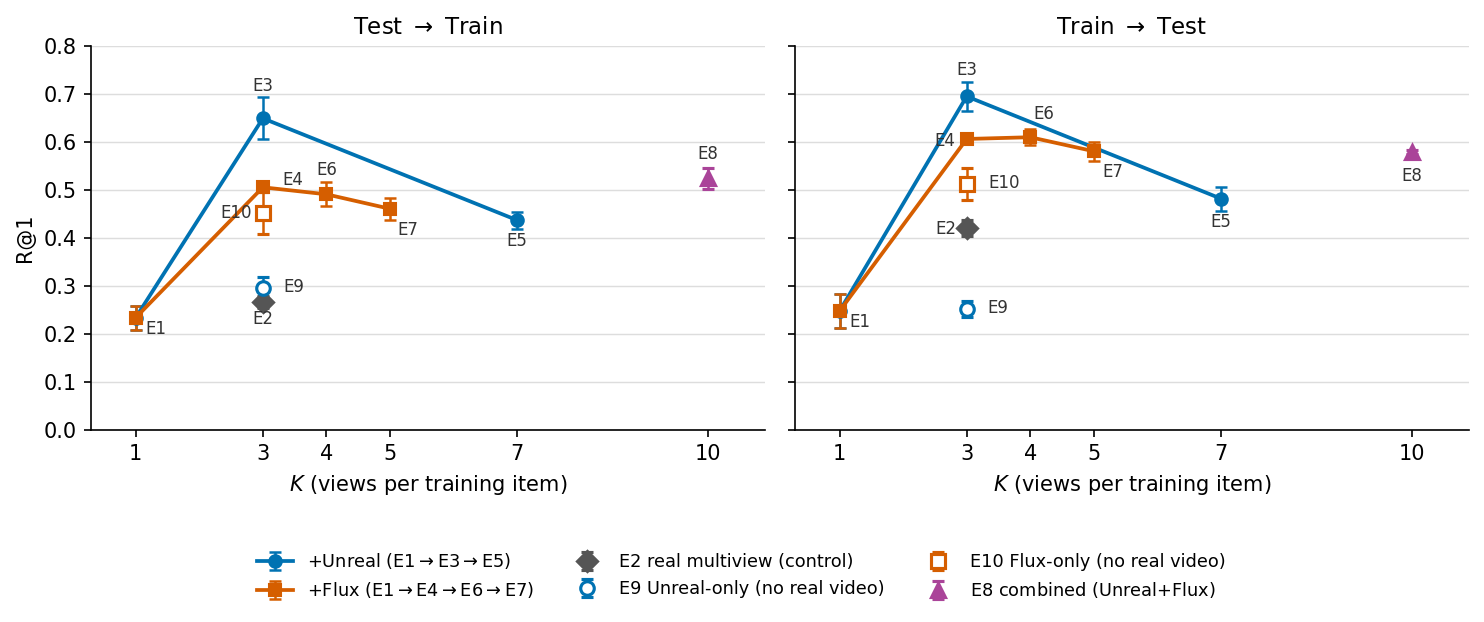
\includegraphics[width=\textwidth]{ngt_synthetic_views_r1_vs_k.png}
\caption[Synthetic-view arms: cross-signer R@1 against views per item]{Synthetic-view arms on NGT744: cross-signer R@1 against the number of
views per training item $K$, by augmentation family (3-seed mean$\pm$sd;
front-view evaluation as in Table~\ref{tab:ngt_synthetic_views}, same 0--1 scale).
Lines trace the
Unreal (E1$\to$E3$\to$E5) and Flux (E1$\to$E4$\to$E6$\to$E7) families from
the shared real-only baseline; isolated points mark the real-multiview
control (E2), the two synthetic-only arms trained without any real video
(E9 Unreal-only and E10 Flux-only, open markers), and the combined arm
(E8). Every arm is drawn at its true $K$, so the five arms that share
$K{=}3$ (E2, E3, E4, E9, E10) sit in one column. The Unreal route peaks
sharply at matched $K{=}3$ and
collapses at full strength ($K{=}7$), whereas the Flux route stays flat as
edits are added.}
\label{fig:ngt_synthetic_views_r1}
\end{figure*}

Figure~\ref{fig:ngt_synthetic_views_r1} plots R@1 against $K$ by
augmentation family, which makes the family structure that
Table~\ref{tab:ngt_synthetic_views} lists row-wise directly visible.
With viewpoint held fixed, both synthetic routes recover a large share of
the cross-signer gap. Over the real-only baseline (E1, test$\to$train R@1
$0.234$), the matched-$K{=}3$ Unreal arm (E3) reaches $0.649$ and the
matched-$K{=}3$ Flux arm (E4) $0.505$: paired gains of $\Delta$R@1
$+0.416$ and $+0.272$ test$\to$train, $+0.448$ and $+0.359$
train$\to$test. Exact McNemar was run on the full-strength arms, where the
substantially smaller gains over E1 (E5 $+0.203$, E6 $+0.257$
test$\to$train) are already significant on $3/3$ seeds in both directions.
At matched strength the motion-locked route wins the head-to-head:
E3 exceeds E4 by $\Delta$R@1 $0.144$ (test$\to$train) / $0.089$ (train$\to$test), significant on
all three seeds test$\to$train and two of three train$\to$test. The generative route therefore
retains roughly $65$--$80\%$ (by
direction) of the Unreal appearance gain at equal $K$, content, and viewpoint:
a substantial but incomplete substitute for the motion-locked renders. Both
synthetic-only arms, trained without any real video (E9 Unreal-only $0.296$, E10
Flux-only $0.452$), at least match the real-only baseline, indicating the avatar
and edited frames carry the discriminative sign content on their own.
Crucially,
the real-multiview control (E2; two \emph{real} extra camera views of the
same signers at the same $K{=}3$) does not reproduce the synthetic gain: it
leaves test$\to$train R@1 near baseline ($0.266$ vs E1 $0.234$) and, while it does lift
train$\to$test ($0.420$ vs $0.247$), stays far below the matched-$K$ synthetic arms in
both directions (E3 $0.649$/$0.695$, E4 $0.505$/$0.606$). Extra viewpoints of the
same identities are therefore not what drives the effect; appearance and
identity diversity is.

Adding synthetic views \emph{beyond} the matched $K{=}3$ does not help, and for
the Unreal route it hurts: the full six-view Unreal arm (E5, $K{=}7$) falls to
R@1 $0.437$, far below its own $K{=}3$ counterpart ($0.649$), whereas the extra
Flux variants (E6--E7) leave the Flux score essentially unchanged. The two
full-strength arms consequently invert the matched-$K$ ordering (E6 $>$ E5,
$\Delta$R@1 $+0.054$/$+0.128$, $2/3$ and $3/3$ seeds), an effect that recurs,
attenuated, on the test-matched subset tier (E6s $>$ E5s, $+0.018$/$+0.065$,
$1/3$ and $2/3$ seeds).

Taken together, the synthetic-view arms separate what viewpoint
diversity contributes from what identity diversity contributes. Adding real
viewpoints does help: the two extra camera views in E2 slightly lift the real-only
baseline (E1) from R@1 $0.234$ to $0.266$ test$\to$train and, far more sharply, from
$0.247$ to $0.420$ train$\to$test ($+0.173$). But the same view budget spent on
identity buys much more: at the identical $K{=}3$, two Unreal avatars
rendered at the unchanged front camera (E3, $0.649$/$0.695$) sit far above the
multiview control in both directions. Nor do synthetic viewpoints stack on
top of synthetic identities: rendering the same avatars from three cameras
(E5, $K{=}7$, $0.437$/$0.482$) lands over $0.2$ R@1 below E3, at
the constant 64-sign negative pool shared by all arms, so negative
starvation cannot account for the drop. The two diversity axes are, however,
not independent: in the signer-count ablation that follows, the
appearance-over-real-viewpoints panel (Table~\ref{tab:ngt_signer_count},
Fig.~\ref{fig:ngt_dropoff}) starts from a stronger real baseline than the
single front view (test$\to$train roughly $0.26$--$0.28$ vs $0.21$--$0.24$, train$\to$test
$0.32$--$0.34$ vs $0.24$--$0.26$ across $S$), and the Unreal gain measured from that
stronger baseline is smaller ($+0.042$ to $+0.109$ R@1 across cells, vs $+0.081$
to $+0.160$ in the appearance $+$ viewpoint panel, E1$\to$E5): real viewpoints already supply part of what the
avatars supply. Real
viewpoints help (mostly train$\to$test), synthetic identities at matched $K$ help
far more, synthetic viewpoints beyond matched $K$ hurt, and viewpoint
diversity partially substitutes for identity diversity.


\subsection{Does the synthetic gain survive real diversity? A fixed-data
real-signer-count ablation}
\label{sec:ngt-signer-count}
% Appearance-only panel provenance: the E3-equivalent arms (ngt_sv_unreal_R1..R4)
% never trained in the first attempt (the jobs died at start on the scratch
% inode quota); retrained 2026-07-29 as Snellius jobs 25042412--25042415
% (3 seeds each) and harvested from ngt_sv_unreal_R*_aggregated.json.
The two-regime reading predicts that the Unreal gain is a property of
\emph{low real-signer diversity}: as genuine signer variety enters
training, synthetic appearance variety should have progressively less to
add. The NGT744 corpus permits a direct test: its training pool comprises
four recording sessions, each a distinct real signer. We propose a
fixed-budget ablation design: we train at
$S \in \{1,2,3,4\}$ real signers, nested (each condition's signers are a
subset of the next), and measure at each $S$ the paired gain
$\Delta(S)$ of two avatar arms over the real-only arm (E1, $K{=}1$): the
appearance-only arm (the synthetic-view E3 setup, $K{=}3$: front camera plus
both avatars' front views) and the full Unreal arm (E5, $K{=}7$).

The load-bearing control is that data volume is fixed while diversity
varies: every condition trains on exactly 180 sentences (the largest even
budget the smallest single-signer pool supports), split evenly across its included signers, with a
single (deterministic, render-complete)
take per sentence, so 180 front-view videos, identical epoch size, and
an identical update budget everywhere, and the take-count differences
between signers (1.5--2.4 takes per sentence) cannot masquerade as a
diversity effect. All arms of a condition use the same sentences and the
same takes; the Unreal arms differ only by attaching avatar views of each
take (the two avatar front views for E3, all six avatar views for E5).


In Table~\ref{tab:ngt_signer_count}, the
real-only arm of each panel barely moves with $S$: spreading the same 180
sentences over one, two, three or four real signers leaves cross-signer
retrieval at R@1 $0.21$--$0.24$ from one real view and $0.26$--$0.28$ from
three (test$\to$train), so real signer variety at constant data volume
does not by itself help. The avatar gain does move, and in the
direction the two-regime account predicts: appearance $+$ viewpoint
shrinks from $+0.145$ at $S{=}1$ to $+0.081$ at $S{=}4$ (test$\to$train),
and appearance over real viewpoints repeats the pattern from a stronger
real baseline with smaller gains throughout. Appearance only stands apart
in size: it is the strongest configuration at every $S$ (R@1
$0.450$--$0.527$ test$\to$train), two to three times the appearance $+$
viewpoint gain, and significant in $3/3$ seeds in every cell.

\begin{table}[t]
\centering
\footnotesize
\begin{tabular}{lccc}
\toprule
$S$ (signers) & real-only arm & $+$avatar arm & $\Delta(S)$ \\
\midrule
\multicolumn{4}{l}{\textbf{Appearance $+$ viewpoint}: 1 real view $\to$ $+$ 6 avatar views \;(E1 $\to$ E5)} \\
\midrule
\multicolumn{4}{l}{\textit{Test $\to$ Train}} \\
1 & 0.237\pmsd{0.007} & 0.382\pmsd{0.022} & $+0.145$ \\
2 & 0.210\pmsd{0.019} & 0.321\pmsd{0.020} & $+0.111$ \\
3 & 0.212\pmsd{0.020} & 0.315\pmsd{0.025} & $+0.103$ \\
4 & 0.224\pmsd{0.011} & 0.305\pmsd{0.029} & $+0.081$ \\
\multicolumn{4}{l}{\textit{Train $\to$ Test}} \\
1 & 0.259\pmsd{0.027} & 0.419\pmsd{0.003} & $+0.160$ \\
2 & 0.236\pmsd{0.017} & 0.392\pmsd{0.058} & $+0.156$ \\
3 & 0.244\pmsd{0.037} & 0.376\pmsd{0.019} & $+0.133$ \\
4 & 0.239\pmsd{0.029} & 0.373\pmsd{0.041} & $+0.134$ \\
\midrule
\multicolumn{4}{l}{\textbf{Appearance only}: 1 real view $\to$ $+$ 2 front avatars \;(E1 $\to$ E3)} \\
\midrule
\multicolumn{4}{l}{\textit{Test $\to$ Train}} \\
1 & 0.237\pmsd{0.007} & 0.527\pmsd{0.044} & $+0.289$ \\
2 & 0.210\pmsd{0.019} & 0.483\pmsd{0.027} & $+0.273$ \\
3 & 0.212\pmsd{0.020} & 0.450\pmsd{0.034} & $+0.238$ \\
4 & 0.224\pmsd{0.011} & 0.482\pmsd{0.061} & $+0.257$ \\
\multicolumn{4}{l}{\textit{Train $\to$ Test}} \\
1 & 0.259\pmsd{0.027} & 0.557\pmsd{0.026} & $+0.298$ \\
2 & 0.236\pmsd{0.017} & 0.524\pmsd{0.040} & $+0.288$ \\
3 & 0.244\pmsd{0.037} & 0.523\pmsd{0.030} & $+0.279$ \\
4 & 0.239\pmsd{0.029} & 0.538\pmsd{0.035} & $+0.299$ \\
\midrule
\multicolumn{4}{l}{\textbf{Appearance over real viewpoints}: 3 real $\to$ $+$6 avatars \;(E2 $\to$ E2$+$av.)} \\
\midrule
\multicolumn{4}{l}{\textit{Test $\to$ Train}} \\
1 & 0.269\pmsd{0.028} & 0.378\pmsd{0.005} & $+0.109$ \\
2 & 0.256\pmsd{0.011} & 0.338\pmsd{0.025} & $+0.082$ \\
3 & 0.257\pmsd{0.032} & 0.337\pmsd{0.035} & $+0.080$ \\
4 & 0.277\pmsd{0.017} & 0.360\pmsd{0.012} & $+0.083$ \\
\multicolumn{4}{l}{\textit{Train $\to$ Test}} \\
1 & 0.322\pmsd{0.040} & 0.429\pmsd{0.015} & $+0.106$ \\
2 & 0.327\pmsd{0.008} & 0.422\pmsd{0.033} & $+0.095$ \\
3 & 0.338\pmsd{0.021} & 0.380\pmsd{0.037} & $+0.042$ \\
4 & 0.344\pmsd{0.014} & 0.394\pmsd{0.021} & $+0.049$ \\
\bottomrule
\end{tabular}
\caption[Real-signer-count ablation on NGT744]{Real-signer-count ablation: cross-signer retrieval R@1 (0--1
scale), mean$\pm$sd over 3 seeds. $\Delta(S)$ is the paired gain of the
$+$avatar arm over the real-only arm in the same panel, from unrounded
means.
Codes name the configurations of
Table~\ref{tab:ngt_synthetic_views} (plus E2$+$av., the E2 arm carrying
the same six avatar views, $K{=}9$), but every arm here is retrained at
the 180-sentence budget, so absolute values differ from that table. Per-seed exact
McNemar ($p<0.05$) holds in $3/3$ seeds for appearance-only everywhere,
$3/3$ for appearance $+$ viewpoint except $S{=}4$ test$\to$train, and
$3/3/2/3$ and $3/2/1/2$ (the two directions) for appearance over real
viewpoints.}
\label{tab:ngt_signer_count}
\end{table}

\begin{figure*}[t]
\centering
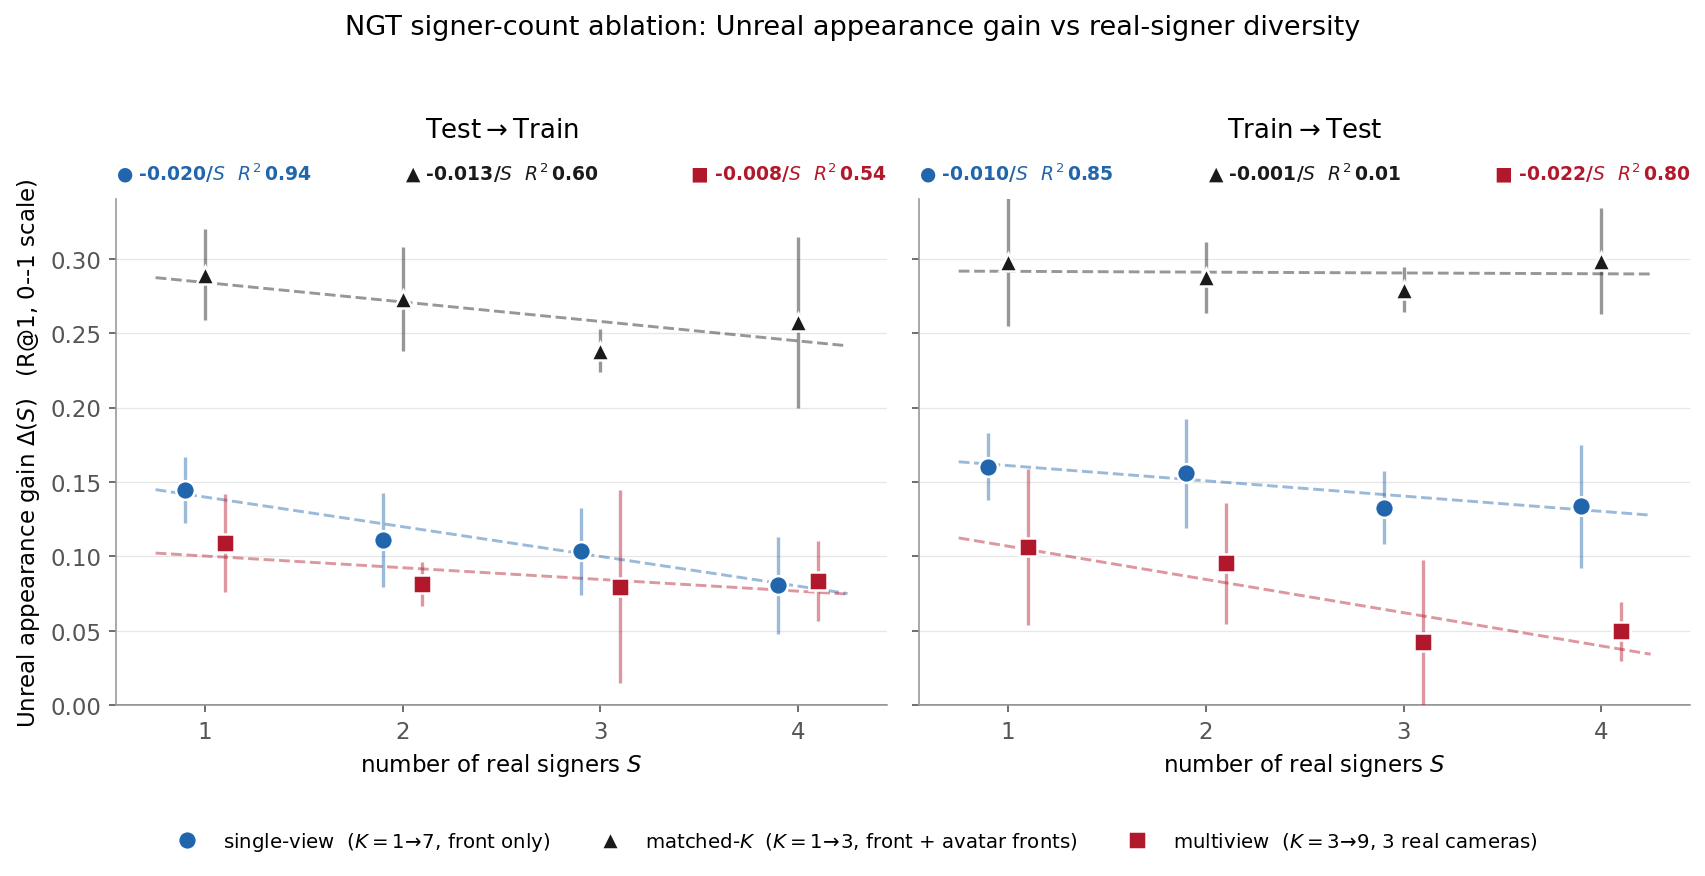
\includegraphics[width=.9\textwidth]{ngt_dropoff.png}
\caption[Unreal appearance gain against real-signer count]{Unreal appearance gain $\Delta(S)$ against real-signer count, for the
three panels of Table~\ref{tab:ngt_signer_count}: appearance $+$ viewpoint
(E1 $\to$ E5), appearance only (E1 $\to$ E3), and appearance over real
viewpoints (E2 $\to$ E2$+$avatars), in each retrieval direction. Dashed
lines are least-squares fits, annotated with slope per added signer and
$R^2$. The two panels whose avatars also add viewpoints shrink as real
signer diversity grows, and the gain measured over the three-real-view
baseline is smaller throughout, both consistent with the two-regime
reading that synthetic appearance variety substitutes for absent real
diversity.}
\label{fig:ngt_dropoff}
\end{figure*}

\section{High-diversity regime: ASL Citizen}
\label{sec:results-highdiv}

\subsection{Direct backbone fine-tuning: an informative null}
We begin by fine-tuning the Logos MViTv2-S
backbone itself with cross-entropy and, optionally, an appearance-invariance
term, then re-evaluate frozen features
with dictionary retrieval and a linear probe on the identical gallery.
Training a
contrastive head on top of the frozen features follows in the next
subsection.
Table~\ref{tab:backbone_ft_retrieval} reports the result. Its rows name what
is added to plain gloss cross-entropy: \emph{CE only} is the unchanged
backbone trained with cross-entropy on the real videos under our recipe,
\emph{$+$ synth.\ data} adds the generative appearance edits as extra training items,
\emph{$+$ cosine consistency}, \emph{$+$ CLS-SupCon} and \emph{$+$ SDDA}
each add the named invariance term on top of real and synthetic data,
and \emph{$+$ gloss-SupCon} adds a supervised-contrastive term over
same-gloss clips (\S\ref{sec:method-losses}).

\begin{table*}[t]
\centering
\footnotesize
\setlength{\tabcolsep}{3pt}
\begin{tabular}{lcccc@{\hskip 1.0em}ccc}
\toprule
 & \multicolumn{4}{c}{\textbf{Dictionary retrieval}} & \multicolumn{3}{c}{\textbf{Linear probe}} \\
\cmidrule(lr){2-5}\cmidrule(lr){6-8}
\textbf{Configuration} & \textbf{DCG} & \textbf{R@1} & \textbf{R@5} & \textbf{R@10} & \textbf{R@1} & \textbf{R@5} & \textbf{R@10} \\
\midrule
\multicolumn{8}{l}{\emph{Reference systems}} \\
\;\;ST-GCN (end-to-end)$^{\dagger}$~\cite{aslcitizen}  & 76.37 & 59.52 & 82.68 & 88.13 & --- & --- & --- \\
\;\;I3D (end-to-end)$^{\dagger}$~\cite{aslcitizen}     & 79.13 & 63.10 & 86.09 & 90.86 & --- & --- & --- \\
\;\;SignRep (frozen)$^{\dagger}$~\cite{wongSignRepEnhancingSelfSupervised2025} & 90.84 & 81.37 & 96.11 & --- & --- & --- & --- \\
\;\;Logos (frozen)~\cite{ovodovLogosWellTemperedPretrain2025} & \textbf{92.73} & \textbf{83.59} & \textbf{98.36} & \textbf{99.04} & \tbest{86.33} & \tbest{98.34} & \tbest{99.00} \\
\midrule
\multicolumn{8}{l}{\emph{Logos fine-tuned, top-2 unfreeze}} \\
% Run-id mapping: CE only=run2, +synth=run3, +cosine=run1,
% +CLS-SupCon=run1_clscontrast, +SDDA=run_sdda; top-6: run2_mid,
% run1_mid; full: run_full_ce, run_full_glosscon, run_full_sdda.
% Retest deltas (old generation values in git, experiments.tex
% pre-07-21): retrieval 0.01-0.30 points, probe 0.05-1.84 points; the
% cosine probe value is the least stable (1.84).
\;\;CE only (standard fine-tuning) & 93.58 & 85.57 & 98.49 & 99.08 & \textbf{86.26} & 97.67 & 98.43 \\
\;\;$+$ synth.\ data (aug-as-data) & \textbf{93.59} & \textbf{85.59} & 98.52 & \textbf{99.11} & 85.76 & 97.30 & 98.14 \\
\;\;$+$ cosine consistency & 93.57 & 85.45 & \textbf{98.55} & 99.06 & 82.27 & 95.37 & 96.61 \\
\;\;$+$ CLS-SupCon & 93.08 & 84.43 & 98.34 & 99.03 & 85.10 & 97.26 & 98.08 \\
\;\;$+$ SDDA & 92.66 & 83.45 & 98.32 & 99.03 & 85.88 & \textbf{97.95} & \textbf{98.67} \\
\midrule
\multicolumn{8}{l}{\emph{Logos fine-tuned, top-6 unfreeze}} \\
\;\;CE only (standard fine-tuning) & \tbest{\textbf{93.78}} & \tbest{\textbf{85.95}} & \textbf{98.48} & \textbf{99.09} & \textbf{85.69} & \textbf{97.13} & \textbf{97.77} \\
\;\;$+$ cosine consistency & 93.62 & 85.63 & \textbf{98.48} & 99.05 & 82.45 & 94.54 & 95.76 \\
\midrule
\multicolumn{8}{l}{\emph{Logos fine-tuned, full unfreeze}} \\
\;\;CE only (standard fine-tuning) & 93.37 & 84.96 & 98.49 & 99.10 & 85.29 & 97.55 & 98.44 \\
\;\;$+$ gloss-SupCon & 93.38 & 84.94 & \tbest{\textbf{98.58}} & \tbest{\textbf{99.12}} & 85.38 & \textbf{97.61} & \textbf{98.51} \\
\;\;$+$ SDDA & \textbf{93.39} & \textbf{85.00} & 98.54 & 99.11 & \textbf{85.55} & 97.60 & 98.46 \\
\bottomrule
\end{tabular}
\caption[Frozen-feature retrieval after backbone fine-tuning]{Dictionary
retrieval and linear-probe accuracy on ASL Citizen after backbone
fine-tuning, all on the identical full gallery; row names are explained
in the text. $^{\dagger}$ marks values taken from the cited papers under
the same retrieval protocol, which report retrieval only, and SignRep
does not report R@10. Bold marks the best value per column within a
block, a blue cell the best in that column table-wide. Every cell is a
single training run, so near-ties should be read as equivalent.
}
\label{tab:backbone_ft_retrieval}
\end{table*}

Before the findings, one framing note: the frozen Logos row is not an
achievement of this thesis. It is the unmodified Logos backbone of
Ovodov et al.~\cite{ovodovLogosWellTemperedPretrain2025}, whose authors
never evaluated on ASL Citizen; that it nonetheless exceeds the
benchmark's published end-to-end baselines and SignRep's frozen
representation, with no target-corpus training at all, is a property of
their pretraining. For this thesis it is the baseline: the bar that
every fine-tuning and augmentation arm below attempts to clear.

Four findings stand out. (i) Cross-entropy fine-tuning improves retrieval R@1
from 83.59 (best frozen) to 85.57 at top-2 depth (85.95 at top-6), while
the linear probe is already best \emph{without} any fine-tuning (86.33):
fine-tuning improves retrieval clustering at a small cost to linear
separability. (ii) Depth helps only up to a point: full unfreeze (84.96)
is worse than top-6 (85.95). (iii) No appearance or
signer-invariance objective beats plain cross-entropy at matched depth,
and several are worse: aug-as-data is statistically indistinguishable
from the matched CE run (85.59 vs 85.57, a gap far below the retest
spread quantified below), SDDA below both (83.45, at
frozen-baseline level). The
matched full-unfreeze pair makes this precise
(gloss-SupCon $\approx$ CE only, $\Delta$R@1$<0.1$ on both evals),
and the per-variant consistency ablations replicate it: all four
single-variant runs (glasses/shirt/signer-swap/skin) land in a 0.14-point
band around the aggregate (retrieval R@1 85.48--85.62), so no individual edit
type carries hidden signal. Four of the top-2 configurations were
trained a second time on independently regenerated edits and reproduced
the pattern; retrieval moved by $0.01$--$0.3$ points and probe values by
up to $1.8$, which is the spread the within-block orderings have to be
read against. (iv) Cosine consistency actively damages the
linear probe (probe R@1 drops to 82.27 at top-2 and 82.45 at top-6,
and it is also the least stable value in the table, moving $1.8$ points
between repeats) while its retrieval score
looks ordinary: the positive-only pull distorts the geometry in a way
nearest-neighbour retrieval tolerates but a linear head does not. The
two-stage schedule (\S\ref{sec:setup-training}: the consistency term
switched on only after CE convergence, at a $100\times$ lower learning
rate) fits the same pattern: its retrieval R@1 of 85.02 sits within the
plain-CE range (84.96--85.95) rather than above it, while its probe R@1
of 85.82 avoids the linear-probe damage of single-stage consistency
training. 
Whether the consistency loss in fact pulls augmented copies together is
taken up in \S\ref{sec:results-ft-probes} and
\S\ref{sec:results-aug-geometry}.

\subsection{SignCLIP head on frozen Logos/I3D features}
We next evaluate the appearance edits as training data for a contrastive
SignCLIP-style head trained on top of frozen backbone features
(Table~\ref{tab:asl_citizen_retrieval}).

Rows are named compositionally. \emph{Synth.} marks any training that uses
the Flux appearance edits: \emph{$+$ synth.\ data} adds them to the real
training videos as extra items, \emph{synth.\ data only} trains on the
edits alone, and the pair-SupCon rows use them as explicit positives
(\S\ref{sec:method-objectives}); unmarked rows train on real videos only.
The three pose rows are the published results of the original SignCLIP
model~\cite{jiangSignCLIPConnectingText2024} rather than our runs, which
is why they are reported to two decimals where ours carry three. The
second block searches over head recipes with the backbone held frozen;
the third then carries two of those recipes, the weakest and the best,
onto backbones we had fine-tuned (CE-FT is cross-entropy on the real
videos, aug-FT adds the synthetic edits as data, SDDA-FT adds the SDDA
invariance term, \S\ref{sec:method-losses}). That third block uses a
different frame preprocessing from the rows above, so it carries its own
frozen-backbone rows and is read within the block.

\todome{REWRITTEN 12.08: the previous version claimed ``the head is worth
adding'', which this table cannot show (every row has a head). It now
describes what the recipes differ in, read off the run configs. Two
things surfaced while checking: \emph{from scratch} initialises both
towers from pretrained BERT rather than randomly, and \emph{synth.\ data
only} trains on 450 of the 2{,}731 glosses, which is the real reason it
scores low. A separate check on whether the recipe search used the
preprocessing the Logos authors use is still open.}
The five rows differ in only two respects: how many training stages the
head gets, and which clips it sees. All of them share the architecture,
the frozen features, the contrastive loss, the batch size and the
evaluation. \emph{From scratch} is a single stage with both towers
initialised from pretrained BERT weights, so it is untrained on sign
language rather than randomly initialised. \emph{Fine-tuned} adds a
second stage that resumes the first at a fifth of the learning rate, with
weight decay and a shorter annealing schedule. \emph{$+$ synth.\ data}
changes nothing but the training split, adding $8{,}989$ edited clips to
the $40{,}154$ real ones. \emph{Synth.\ data only} replaces the real
videos with the edits, and is not a like-for-like comparison: the edited
subset covers $450$ of the $2{,}731$ glosses, so that row trains on a
sixth of the vocabulary.

Read this way, the second stage is worth $3.9$ points ($0.750$ to
$0.789$) and the edits roughly one more on top of it ($0.789$ to
$0.800$), while the vocabulary-limited row ($0.760$) says nothing about
how good the edits are. All of these are small beside the choice of
features underneath: the same head reaches $0.32$ on I3D features against
$0.750$ on frozen Logos ones, and the published pose-input SignCLIP
models $0.39$--$0.60$.

Carrying those recipes onto fine-tuned backbones shows that the two do
not stack. A from-scratch head does gain from a fine-tuned backbone ($0.744$
on the matched frozen control against $0.772$--$0.782$), but the best head
recipe does not: it scores highest on the frozen backbone ($0.818$) and
slightly lower on every fine-tuned one ($0.809$--$0.812$). Whatever
backbone fine-tuning has to contribute at this point, the head has
already contributed.

The pair-SupCon rows are the largest effect in the table, and they are a
clean comparison: they resume the same from-scratch head as the
fine-tuned rows, so all of these runs are second stages from one
checkpoint and differ only in what that stage optimises. Keeping the
video--text loss and adding the edits as data carries the head from
$0.750$ to $0.800$. Replacing that loss with SupCon over each video and
its own edits leaves it below where it started: $0.567$ with two edits
and $0.414$ with four. The same clips therefore help or hurt according to
the objective they enter through, and within the SupCon runs more of them
is worse (\S\ref{sec:results-iconicity-main} returns to why).

% TABLE CONVENTION (updated 2026-08-05 per Piotr):
% - \textbf on a data cell = best value in that metric column within its
%   comparison block (ties: all bolded).
% - \tbest{...} (blue cell) = best value in that column across the WHOLE
%   table (per eval type, individual cells; Med.R skipped where all-tied).
% - \rowcolor{rowhl} = the recommended configuration overall (may differ
%   from per-column winners; say so in the caption if it does).
% - Stub column header is "Setup"; setup labels are compositional:
%   {From scratch | Fine-tuned} x {(real only) | + synth. data | , synth.
%   data only}, "synth. data" (not "aug") everywhere.
% Applied so far: T2V table + stub headers of both retrieval tables.
% Remaining tables to be swept for per-block bolding (Phase 2).
\begin{table*}[t]
\centering
\footnotesize
\setlength{\tabcolsep}{3pt}
\begin{tabular}{llcccc}
\toprule
\textbf{Setup} & \textbf{Backbone} & \textbf{R@1} & \textbf{R@5} & \textbf{R@10} & \textbf{Med.\,R} \\
\midrule
\multicolumn{6}{l}{\textit{Published SignCLIP baselines}} \\
SignCLIP from scratch        & MediaPipe pose & 0.39 & 0.71 & 0.84 & 2 \\
SignCLIP fine-tuned          & MediaPipe pose & 0.46 & 0.77 & 0.84 & 2 \\
SignCLIP fine-tuned + linear & MediaPipe pose & \textbf{0.60} & \textbf{0.84} & \textbf{0.89} & 1 \\
\midrule
\multicolumn{6}{l}{\textit{Head-recipe search, backbone frozen}} \\
From scratch          & I3D                  & 0.32  & 0.63  & 0.73  & 3 \\
From scratch          & Logos (frozen) & 0.750 & 0.950 & 0.970 & 1 \\
From scratch $+$ synth.\ data & Logos (frozen) & 0.756 & 0.955 & 0.970 & 1 \\
Fine-tuned            & Logos (frozen) & 0.789 & 0.962 & 0.975 & 1 \\
Fine-tuned, synth.\ data only & Logos (frozen) & 0.760 & 0.957 & 0.971 & 1 \\
Fine-tuned $+$ synth.\ data & Logos (frozen) & \textbf{0.800} & \textbf{0.964} & \textbf{0.976} & 1 \\
\midrule
\multicolumn{6}{l}{\textit{The same recipes on fine-tuned backbones}$^{\ddagger}$} \\
From scratch              & Logos (frozen)   & 0.744 & \textbf{0.966} & \textbf{0.977} & 1 \\
From scratch              & Logos (CE-FT)    & 0.772 & 0.929 & 0.944 & 1 \\
From scratch              & Logos (aug-FT)   & 0.781 & 0.927 & 0.943 & 1 \\
From scratch              & Logos (SDDA-FT)  & \textbf{0.782} & 0.958 & 0.970 & 1 \\
\addlinespace
\rowcolor{rowhl}
Fine-tuned $+$ synth.\ data & Logos (frozen)   & \tbest{\textbf{0.818}} & \tbest{\textbf{0.972}} & \tbest{\textbf{0.982}} & 1 \\
Fine-tuned $+$ synth.\ data & Logos (CE-FT)    & 0.809 & 0.946 & 0.957 & 1 \\
Fine-tuned $+$ synth.\ data & Logos (aug-FT)   & 0.812 & 0.942 & 0.954 & 1 \\
Fine-tuned $+$ synth.\ data & Logos (SDDA-FT)  & 0.810 & 0.964 & 0.974 & 1 \\
\midrule
\multicolumn{6}{l}{\textit{Pair-SupCon head (fine-tune; synth.\ edits as explicit positives)}} \\
$K{=}3$ pair-SupCon (orig.\ $+$ 2 edits)        & Logos (frozen) & 0.567 & 0.887 & 0.934 & 1 \\
$K{=}5$ pair-SupCon (orig.\ $+$ 4 edits)        & Logos (frozen) & 0.414 & 0.767 & 0.858 & 2 \\
\bottomrule
\end{tabular}
\caption[Video-to-text retrieval on ASL Citizen]{Video-to-text
retrieval on ASL Citizen; row naming is explained in the text.
$^{\ddagger}$This block uses a different frame preprocessing from the rows
above, so read it against its own frozen-backbone rows rather than against
the earlier numbers. Bold marks the best value per column within a block,
a blue cell the best in the column, and the shaded row the strongest
configuration.}
\label{tab:asl_citizen_retrieval}
\end{table*}


\paragraph{The effect of augmentations on T2V retrieval performance}
\todome{CORRECTED 12.08: this paragraph said ``fine-tuning alone lifts''
(it is the head's second training stage, not backbone fine-tuning) and
read the synth-only row as evidence that synthetic data adds little,
which it cannot be, since that run sees 450 of the 2{,}731 glosses.}
Table~\ref{tab:asl_citizen_t2v} repeats the comparison in the
text-to-video direction, where precision@$k$ replaces recall@$k$: the
gallery holds several correct videos per gloss query, so recall@1 is
capped by gallery multiplicity however good the model is, while
precision@$k$ measures directly whether the top-ranked videos are
correct. The original SignCLIP work does not report this direction on ASL
Citizen at full scale. The ordering
matches the video-to-text table: the second training stage lifts P@1 from
$0.871$ to $0.895$, adding the edits as data during that stage lifts it
again to $0.919$, the strongest configuration on every metric (Mean~R
$1.128$), and adding them during the first stage instead is worth less
($0.883$). The vocabulary-limited row ($0.884$) is no more comparable
here than it was above. Carried onto the fine-tuned backbones, the same recipe reaches
P@1 $0.925$--$0.935$, mirroring its video-to-text behaviour. Which backbone leads does depend on the direction, however: the frozen
backbone is strongest video-to-text ($0.818$ against $0.809$ on CE-FT)
while CE-FT is strongest text-to-video ($0.935$ against $0.925$), so the
shaded row differs between the two tables.
\todome{DRAFT PROPOSAL END. Interpretive reading (why T2V moves more
than V2T --- the anchor-neighbourhood argument) was cut in the 03.08
cleanup; reconnect it here or leave the paragraph descriptive.}

\begin{table*}[t]
  \centering
  \small
  \makebox[\linewidth][c]{
  \begin{tabular}{llcccc}
  \toprule
  \textbf{Setup} & \textbf{Backbone} & \textbf{P@1} & \textbf{P@5} & \textbf{P@10} & \textbf{Mean R} \\
  \midrule
  From scratch          & Logos (frozen) & 0.871 & 0.854 & 0.786 & 1.228 \\
  From scratch $+$ synth.\ data    & Logos (frozen) & 0.883 & 0.861 & 0.790 & 1.213 \\
  Fine-tuned           & Logos (frozen) & 0.895 & 0.876 & 0.808 & 1.166 \\
  Fine-tuned, synth.\ data only & Logos (frozen) & 0.884 & 0.863 & 0.796 & 1.216 \\
  Fine-tuned $+$ synth.\ data      & Logos (frozen) & \textbf{0.919} & \textbf{0.896} & \textbf{0.829} & \textbf{1.128} \\
  \midrule
  \multicolumn{6}{l}{\textit{The best recipe on fine-tuned backbones}} \\

  Fine-tuned $+$ synth.\ data & Logos (frozen)   & 0.925 & 0.902 & \tbest{\textbf{0.850}} & 1.129 \\
  Fine-tuned $+$ synth.\ data & Logos (CE-FT)    & \tbest{\textbf{0.935}} & 0.909 & 0.844 & 1.106 \\
  Fine-tuned $+$ synth.\ data & Logos (aug-FT)   & 0.930 & \tbest{\textbf{0.910}} & 0.848 & \tbest{\textbf{1.099}} \\
  Fine-tuned $+$ synth.\ data & Logos (SDDA-FT)  & 0.928 & 0.906 & 0.849 & 1.112 \\
  \bottomrule
  \end{tabular}
  }
  \caption[Text-to-video retrieval on ASL Citizen]{Text-to-video
  retrieval on ASL Citizen, same configurations as
  Table~\ref{tab:asl_citizen_retrieval} and the same marking convention.}
  \label{tab:asl_citizen_t2v}
\end{table*}

A qualitative view of the gloss organisation of nine of these spaces,
projected with t-SNE on a shared clip sample, is given in
Appendix~\ref{app:tsne_grid}.


\subsection{Does any objective actually remove signer identity? Distance and
decoding probes on the fine-tuned spaces}
\label{sec:results-ft-probes}
The retrieval numbers above measure task quality, not signer encoding: a
fine-tuned space can match the baseline's accuracy while carrying just as
much identity information. We therefore probe every re-extracted space $z$
with two complementary readouts. The \emph{distance probe} repeats the
construction of \S\ref{sec:results-l2-raw} on each space: per test video the
mean L2 distance to same-gloss clips by the \emph{same} signer
($\bar{d}_{\mathrm{intra}}$) versus by \emph{different} signers
($\bar{d}_{\mathrm{inter}}$), summarised as the median ratio
$\rho=\mathrm{med}\,\big(\bar{d}_{\mathrm{inter}}/\bar{d}_{\mathrm{intra}}\big)$;
$\rho\!\approx\!1$ means signers are no longer geometrically separated at
fixed sign. The \emph{decoding probe} is its supervised complement, using standard
linear-probing methodology~\cite{alainUnderstandingIntermediateLayers2017}: a linear
head $p(s\,|\,z)=\mathrm{softmax}(Wz+b)$ is trained (cross-validated, frozen
$z$) to predict the signer label $s$, reporting top-1 accuracy against the
$1/S$ chance level. The two can dissociate (a distance probe misses
identity information that is linearly decodable but small relative to
gloss variation), so an intervention that genuinely removes appearance
identity must lower both, not merely rescale distances. We run both probes
on the frozen baseline, the top-2 family (CE, aug-as-data,
cosine-consistency plus its per-variant ablations, SDDA), and the SignCLIP
heads, reading each family as a matched block; the depth confound forbids
comparing across them. The backbone-family probes use the test split; the
SignCLIP-head spaces are exported for the train split only, so their probes
run on the matched train split (35 signers) and are reported as a separate
panel (Table~\ref{tab:head_signer_probes}) that must not be compared
row-for-row with the test-split numbers. The full-unfreeze runs are not probed: their
contribution is already settled at the accuracy level
(Table~\ref{tab:backbone_ft_retrieval}: gloss-SupCon adds nothing even at full
capacity), and the compute budget was spent where new evidence was possible,
so the probe conclusions below are scoped to top-2 depth.
\begin{table}[t]
\centering
\small
\begin{tabular}{lcc}
\toprule
\textbf{Space} & \textbf{$\rho$ (inter/intra)} & \textbf{signer decoding} \\
\midrule
Logos (frozen) & 17.67$\times$ & 75.3\% \\
% run-id mapping as in tab:backbone_ft_retrieval
fine-tuned, CE only       & 16.46$\times$ & 64.2\% \\
fine-tuned $+$ synth.\ data & 16.44$\times$ & 62.6\% \\
fine-tuned $+$ cosine consistency & 16.66$\times$ & 56.3\% \\
fine-tuned $+$ SDDA       & 17.12$\times$ & 67.6\% \\
\bottomrule
\end{tabular}
\caption[Signer-identity probes on the fine-tuned spaces]{Signer-identity probes on the re-extracted top-2-family spaces.
$\rho$ = median over multi-signer glosses of the inter-signer/intra-signer
L2 ratio (prototype-based); in every space 100\% of glosses have
inter $>$ intra. Decoding = linear-head top-1 signer accuracy
(3-fold stratified CV; test split, 11 signers, chance 0.091).}
\label{tab:signer_probes}
\end{table}

\begin{table}[t]
\centering
\small
\begin{tabular}{lcc}
\toprule
\textbf{Head space (train split)} & \textbf{$\rho$ (inter/intra)} & \textbf{signer decoding} \\
\midrule
frozen backbone (reference)        & 17.67$\times^{\dagger}$ & 66.9\% \\
From scratch                       & 22.29$\times$ & 22.6\% \\
Fine-tuned                         & 22.35$\times$ & 24.6\% \\
Fine-tuned $+$ synth.\ data        & 22.02$\times$ & 22.4\% \\
$K{=}3$ pair-SupCon                & 23.35$\times$ & 20.1\% \\
$K{=}5$ pair-SupCon                & 26.34$\times$ & 21.2\% \\
\bottomrule
\end{tabular}
\caption[Signer-identity probes on the SignCLIP-head spaces]{The same two probes on the SignCLIP-head spaces. Head features
exist only for the train split, so this panel uses the matched train
split (35 signers, chance 0.029) and is not comparable row-for-row with
the test-split panel above; the frozen-backbone row gives the same-split
decoding reference. $^{\dagger}$Reference $\rho$ from the full-split
computation above. The dissociation sharpens in the heads: they separate
signers \emph{more} geometrically than the backbone spaces
($\rho$ 22.0--26.3$\times$) while making identity far \emph{less}
linearly decodable (20--25\% against 66.9\% on the same
split).\todo{framing check}}
\label{tab:head_signer_probes}
\end{table}


The two probes dissociate exactly as anticipated. The distance probe says
essentially nothing moved: signer separation at fixed sign is enormous in
the frozen space ($\rho = 17.7\times$, inter-signer prototype distances
exceeding within-signer spread for \emph{every} multi-signer gloss) and
remains so after every fine-tuning objective, with the invariance-targeted
runs sitting at $16.4$--$17.1\times$, indistinguishable from plain CE
($16.5\times$) and barely below frozen. The decoding probe tells a
sharper story: a linear head recovers signer identity from the frozen
space at 75.3\% (11-way chance 9.1\%), and every fine-tuned space is
substantially less decodable: CE alone already drops this to 64.2\%,
aug-as-data to 62.6\%, and cosine consistency furthest, to 56.3\%, while
SDDA is the weakest intervention at 67.6\% despite its loss explicitly
targeting signer structure. So identity is not literally frozen in place:
fine-tuning, and consistency training most of all, measurably erodes the
\emph{linearly decodable} component of signer identity, in a direction
this coarse distance statistic is too blunt to register. This reduction
does not translate into better retrieval (Table~\ref{tab:backbone_ft_retrieval}:
consistency training is at or below plain CE on both evals), so removing
decodable signer information and improving retrieval accuracy are
dissociable outcomes here, consistent with the geometry of
\S\ref{sec:results-aug-geometry}, where the same objectives are shown to
pull their own training pairs together without closing the gap on
held-out counterfactuals.

\subsection{Where do the appearance counterfactuals land? Feature-space
geometry of the augmentations}
\label{sec:results-aug-geometry}
\todo{this is too long and too dense. Decide what is the most relevant, degrade the rest to appendix}
The interventions above add little in the high-diversity regime (\S\ref{sec:results-highdiv}),
and two very different geometries could produce a null of this shape. The
synthetic edits might be \emph{redundant} (each augment landing so close
to its source video that it supplies no variation the backbone has not
already absorbed from a 35-signer corpus), or they might carry a
\emph{sim-to-real gap}: occupying a systematically distinct, ``synthetic''
region of the feature space that adds domain shift rather than useful signer
diversity. These are not mutually exclusive; the more interesting possibility
is their conjunction, in which each augment sits near its own original yet all
augments are collectively separable from real video by a small, shared
offset. Closing exactly this kind of real--synthetic gap is the explicit
target of adversarial synthetic-data methods such as
SDDA~\cite{fuSignerDiversitydrivenData2024b}, and pairing an image with its
counterfactual is the basis of counterfactual-contrastive
learning~\cite{roschewitzCounterfactualContrastiveLearning2025}; here we
instead \emph{measure} the geometry directly.

Every video $v$ is embedded by the backbone under analysis into a single
vector $f(v)\in\mathbb{R}^{768}$ (clip features mean-pooled over the video).
Each Flux edit of type
$t\in\{$shirt, glasses, skin~tone, signer~swap$\}$
yields a pair $\big(f(v),f(\tilde{v}_t)\big)$, matched by video id, and the
object of study is the \emph{displacement}
$\delta_t(v)=f(\tilde{v}_t)-f(v)$, the arrow the edit draws in feature
space. We propose four measurements to characterise these arrows; headline
numbers are medians over pairs.

\textbf{(1) Displacement, in units of a real signer change.} A raw cosine
$\cos\big(f(v),f(\tilde{v}_t)\big)$ is not interpretable on its own
(embedding spaces concentrate similarity, and the concentration differs
between spaces), so we calibrate it against a reference built from the
same features and metadata. For each source $v$ we measure its mean cosine
$\bar{c}(v)$ to up to $64$ videos of the \emph{same gloss by different
signers}, the natural magnitude of a genuine signer change for that very
video. We propose the \emph{normalised displacement}
$\mathrm{n.disp}=\big(1-\cos(f(v),f(\tilde{v}_t))\big)/\big(1-\bar{c}(v)\big)$
to measure the fraction of a real signer change that the edit induces. A value of
$0.5$ means the edit moves the embedding half as far as replacing the
person would; $1.0$, exactly as far. A second per-video control,
\emph{different glosses by the same signer}, provides a sign-identity
floor: in every space and on both samples, $\geq 99.9\%$ of augments remain
closer to their source than this floor: no edit moves a video past its
own sign.

\textbf{(2) Sim-to-real separability.} To test for a collectively
``synthetic'' region we train a standard linear classifier (logistic
regression on
standardised features) to label real originals vs.\ augments, and report
ROC-AUC under a protocol we propose for such paired data: $5$-fold
cross-validation \emph{grouped by source video}, so that a
video and its own edits always occupy the same fold. The grouping is what
makes the number meaningful. An original and its augment are
near-duplicates, so if one fell in the training fold and the other in the
test fold, the classifier could recognise the test item purely by its
proximity to a memorised training item, inflating AUC without any
generalising real-vs-synthetic direction; with grouping, AUC is the
probability that an augment of an \emph{unseen} video scores more
``synthetic'' than an unseen real one ($0.5$ = indistinguishable). We
report AUC on raw and on $\ell_2$-normalised features: a gap that survives
normalisation is directional, whereas one that vanishes was mere feature
magnitude.

\textbf{(3) The de-shift test: is the gap a single translation?} Write
$f(\tilde{v}_t)=f(v)+\mu_t+\varepsilon$. If the synthetic region were
nothing but the shared offset $\mu_t$, subtracting it should erase
separability. Within each cross-validation fold we estimate $\hat{\mu}_t$
as the mean displacement of the \emph{training-fold pairs only}, subtract
it from every augment, retrain, and score on the held-out fold;
estimating the shift on the evaluation pairs themselves would trivially
centre them, so the fold-internal protocol keeps the test honest (and
each training pair contributes only one of its two members, chosen at
random, since keeping both would equalise the class means by construction
and pin AUC at $0.5$ mechanically). A collapse of
AUC$_{\text{de-shift}}$ to chance means the entire linearly detectable
synthetic signature was one translation per edit type.

\textbf{(4) Meaning kept, appearance moved?}
Two checks. \emph{gloss@1}: does the augment's nearest real video
(source excluded) show the same sign? If so, the edit preserved meaning; the
video-to-video analogue of the counterfactual check in
\S\ref{sec:results-diagnosis}. \emph{flip}: summarising each signer by the
mean embedding of their videos (prototype), the share of pairs whose
nearest prototype differs between source and augment, meaning the edit visibly
moved identity-related appearance (intended for signer swap; unintended
drift for the local edits).
Because the whole analysis runs per feature space, we repeat it on the
fine-tuned backbones of Table~\ref{tab:backbone_ft_retrieval}
(aug-as-data, cosine-consistency, SDDA, and the CE control) to ask whether
any intervention pulls the augments toward their originals or shrinks the
synthetic region, the geometric companion to the retrieval numbers.

\textbf{Two evaluation samples.} We evaluate every space on two disjoint
pair samples. The first comprises the $6{,}000$ augmented training source
videos, each with all four edits; it maximizes statistical power but is
selection-biased by construction, since augmentation targets were chosen
worst-first: the classes with the fewest training signers and lowest
baseline accuracy (\S\ref{sec:method-diffusion}). The second is a
signer-stratified random sample of $500$ \emph{test-split} videos, augmented
with the identical pipeline; its signers are fully disjoint from the $35$
training signers. For the frozen backbone (which never saw ASL Citizen,
so neither sample raises a leakage concern), the held-out sample serves as
a check that conclusions are not artifacts of the rare-gloss selection. For
the fine-tuned spaces the distinction is substantive: the training pairs are
the very items those models optimized on, so they bound the intervention's
effect from above, while the held-out pairs give the honest generalization
number; and a divergence between the two is itself informative,
separating memorization of specific counterfactual pairs from a learned
appearance invariance. Both sides of every pair share identical
aspect-preserving spatial preprocessing and a matched effective frame rate,
so the measured displacement contains no framing or temporal-sampling
artifact. What we deliberately do \emph{not} remove is the editing
pipeline's own low-level footprint: every augment passes through a resize to
longest-side $512$ and the generator's encode--decode round trip, and so
carries a faint resampling texture even in pixels the edit left untouched.
That footprint is part of the synthetic signal being measured, because any
model trained on these augments consumes exactly the same footprint; we
verified separately that the saved augments preserve the source aspect
ratio.

We expect the four edit types to fall on a clear ordering: shirt and glasses
are local edits that should displace the embedding only slightly, whereas
skin-tone and signer-swap are whole-person edits that should move it much
further, approaching the magnitude of a genuine signer change. The decisive
question for this null is \emph{where} that displacement lands. If
real-versus-synthetic separability is low, the counterfactuals are faithful and the null is one of
saturation: the high-signer ASL Citizen backbone had already learned the
invariance the edits supply, consistent with the marginal
Table~\ref{tab:asl_citizen_retrieval} gain and with the opposite,
low-signer NGT744 result (\S\ref{sec:results-lowdiv}). If instead the
displacement is highly separable, the edits
carry a sim-to-real gap that offsets their benefit in feature space. This is
the mechanistic evidence behind the reading in
\S\ref{sec:discussion-regimes}.
\begin{table}[t]
\centering
\footnotesize
\setlength{\tabcolsep}{4pt}
\begin{tabular}{lccccc}
\toprule
\textbf{Edit type} & \textbf{n.disp} & \textbf{AUC} &
\textbf{AUC$_{\text{de-shift}}$} & \textbf{gloss@1} & \textbf{flip} \\
\midrule
\multicolumn{6}{l}{\emph{Training pairs ($6{,}000$ per edit type, selection-biased)}} \\
\;\;glasses     & 0.46 & 0.993 & 0.50 & 0.58 & 0.67 \\
\;\;shirt       & 0.53 & 0.999 & 0.50 & 0.62 & 0.76 \\
\;\;skin tone   & 0.44 & 0.997 & 0.51 & 0.63 & 0.68 \\
\;\;signer swap & 1.04 & 1.000 & 0.51 & 0.49 & 0.91 \\
\midrule
\multicolumn{6}{l}{\emph{Held-out test pairs ($500$ per edit type, signer-disjoint)}} \\
\;\;glasses     & 0.50 & 0.960 & 0.50 & 0.70 & 0.57 \\
\;\;shirt       & 0.47 & 0.990 & 0.50 & 0.75 & 0.56 \\
\;\;skin tone   & 0.46 & 0.972 & 0.50 & 0.74 & 0.54 \\
\;\;signer swap & 1.05 & 1.000 & 0.50 & 0.59 & 0.77 \\
\bottomrule
\end{tabular}
\caption[Augmentation geometry in the frozen Logos space]{Augmentation geometry in the \textbf{frozen} Logos space
(fine-tuned spaces: Table~\ref{tab:aug_geometry_spaces}). All values are
medians over pairs. n.disp = displacement as a fraction of a real signer
change (measurement 1); AUC = real-vs-synthetic linear separability under
$5$-fold cross-validation grouped by source video ($\ell_2$-normalised
features change no value by more than $0.001$); AUC$_{\text{de-shift}}$ =
the same test after removing the fold-estimated mean displacement
(measurement 3); gloss@1 = share of augments whose nearest real video
(source excluded) shows the same sign; flip = share of augments nearest to
a different signer's prototype than their source.}
% E_signer removed 2026-08-03 per Piotr's decision; anchors that
% falsified the directional reading: chance 0.012, real signer change
% 0.074, edits 0.09-0.14 (probe_out/esigner_anchors.json, job 25195647).
\label{tab:aug_geometry_frozen}
\end{table}

The frozen-space geometry (Table~\ref{tab:aug_geometry_frozen}) settles
the two hypotheses in favour of their \emph{conjunction}, with one twist.
The locality ordering holds: garment and skin edits move an embedding
about half as far as a genuine signer change (normalised displacement
$0.44$--$0.53$), while signer swap moves it exactly as far as one
($1.04$--$1.05$) and flips the nearest signer prototype for $91\%$ of
training pairs: the intended identity change registers. Sign content
survives every edit (gloss retention $0.70$--$0.75$ on the unbiased
held-out pairs; lower, $0.49$--$0.63$, on the training pairs, which by
construction target the hardest classes).
\todome{NUMBERS BUG (03.08, verified against the table above): held-out
gloss@1 is $0.70$/$0.75$/$0.74$ for glasses/shirt/skin tone but
$\mathbf{0.59}$ for signer swap --- the quoted $0.70$--$0.75$ silently
drops the signer-swap value while the sentence claims content ``survives
every edit''. Proposed rewrite: ``Sign content largely survives the
appearance edits (gloss retention $0.70$--$0.75$ on held-out pairs for
glasses/shirt/skin tone) but takes a real hit from the identity change
($0.59$ for signer swap); on the training pairs, which by construction
target the hardest classes, retention is $0.49$--$0.63$.'' The drop is
worth owning: the strongest edit type also costs the most sign content,
which connects to the hallucination limitation.} Yet the same augments are
near-perfectly linearly separable from real video (AUC $0.96$--$1.00$,
unchanged by $\ell_2$-normalisation, so the gap is directional rather
than a magnitude artifact): each counterfactual sits close to its source
while the synthetic population as a whole occupies an identifiable
region.
The twist is how \emph{shallow} that region's signature is.
After subtracting a single mean displacement vector per edit type,
estimated leak-free within each fold, separability collapses to chance
($0.48$--$0.51$) in every space and on both samples: to linear probing,
the entire sim-to-real gap is one shared translation. The individual
arrows do scatter widely around that translation (the shared
component is only $32$--$53\%$ of a typical displacement's length, and
no single principal direction explains more than about $10\%$ of the
displacement cloud's variance), but the scatter carries no class
information; everything a linear probe can use is the mean offset. This
is the mechanistic reading behind the null: the entire
linearly detectable synthetic signature is a single shared offset per
edit type, a direction a classifier can trivially factor out.

\begin{table}[t]
\centering
\footnotesize
\setlength{\tabcolsep}{4pt}
\begin{tabular}{lcccc}
\toprule
\textbf{Space} & \textbf{n.disp} & \textbf{gloss@1} & \textbf{AUC} &
\textbf{AUC$_{\text{de-sh}}$} \\
\midrule
\multicolumn{5}{l}{\emph{Training pairs}} \\
\;\;frozen      & 1.04 & 0.49 & 0.997 & --   \\
\;\;CE          & 1.13 & 0.56 & 0.992 & --   \\
\;\;aug-as-data & 1.04 & 0.91 & 0.991 & --   \\
\;\;consistency & 0.79 & 0.89 & 0.986 & --   \\
\;\;SDDA        & 0.76 & 0.67 & 0.996 & --   \\
\midrule
\multicolumn{5}{l}{\emph{Held-out pairs}} \\
\;\;frozen      & 1.05 & 0.59 & 0.976 & 0.50 \\
\;\;CE          & 1.00 & 0.60 & 0.972 & 0.50 \\
\;\;aug-as-data & 1.17 & 0.62 & 0.949 & 0.48 \\
\;\;consistency & 1.11 & 0.57 & 0.942 & 0.49 \\
\;\;SDDA        & 0.80 & 0.66 & 0.961 & 0.50 \\
\bottomrule
\end{tabular}
\caption[Augmentation geometry across feature spaces]{The same geometry across feature spaces, shown for the
signer-swap edit (the strongest intervention; the local edits show the
same pattern; full grid with uncertainty in
Appendix~\ref{app:aug_geometry_grid}). n.disp and gloss@1
as in Table~\ref{tab:aug_geometry_frozen}; AUC pools all four edit
types; AUC$_{\text{de-sh}}$ is on held-out
pairs only because, unlike n.disp and gloss@1, it shows no
training/held-out asymmetry to report (training values within $0.03$
in every space). Reading: a model that \emph{learned} appearance invariance would
contract n.disp and preserve gloss@1 in \emph{both} panels;
gains confined to the training panel (aug-as-data, consistency) are
memorisation of the specific counterfactual pairs seen in training. The
CE control never trained on augments and is correspondingly symmetric.}
\label{tab:aug_geometry_spaces}
\end{table}


Qualitative companions to these numbers (a t-SNE of the augments around their source videos and the per-edit-type cosine distributions) are shown in Appendix~\ref{app:aug_geometry_grid} (Figs.~\ref{fig:aug_vs_orig_tsne} and~\ref{fig:aug_vs_orig_cosine}).


\subsection{Iconicity analysis}
\label{sec:results-iconicity-main}
The organising
construct of the Logos dataset is the \emph{visually similar sign}
(VSSign): signs that are made with the same hands, movement and location
but mean different things, whether because one form carries several
related meanings or because two separate signs differ too slightly to
tell apart on video. Logos authors show
that \emph{grouping} VSSigns under one label (training the encoder
precisely \emph{not} to separate signs that look alike) yields a
better transfer encoder than keeping them
apart~\cite{ovodovLogosWellTemperedPretrain2025}. A backbone
pre-trained this way is not merely agnostic about form-similar pairs;
collapsing them is part of its supervision, and that metric bias
travels with the frozen features from RSL to our ASL inputs.
To measure that bias we use ASL-LEX~2.0, a linguistic database that codes
each of $2{,}723$ ASL signs on five phonological features (movement,
major and minor location, handshape, sign type) and rates its iconicity,
how much its form resembles its meaning, from $1$ to
$7$~\cite{sehyrASLLEX2021,caselliASLLEX2017}. The idea is close to the
VSSign one, but the use is not: Logos groups look-alike signs in order to
train on them, whereas we only measure, and counting shared features
turns ``looks alike'' into a scale from zero to five instead of a
yes/no. ASL Citizen is also a corpus Logos never trained on, in a
different language, recorded under different conditions, so what the
measurement asks is whether the form grouping survived that transfer.

ASL Citizen contains such form-similar groups too, and they sit at the top
of the iconicity scale. Figure~\ref{fig:iconicity_family} shows one:
GUN1, LIGHTER and REMOTECONTROL agree on all five features (neutral
location, \texttt{a} handshape, no path movement, one-handed) because
each depicts handling the object it names, and all three rate $5.3$--$5.6$
for iconicity. Iconic vocabulary is exactly where distinct meanings
converge on the same form, so how a space treats form-similar pairs
decides what it can say about iconic signs.

\begin{figure}[t]
\centering
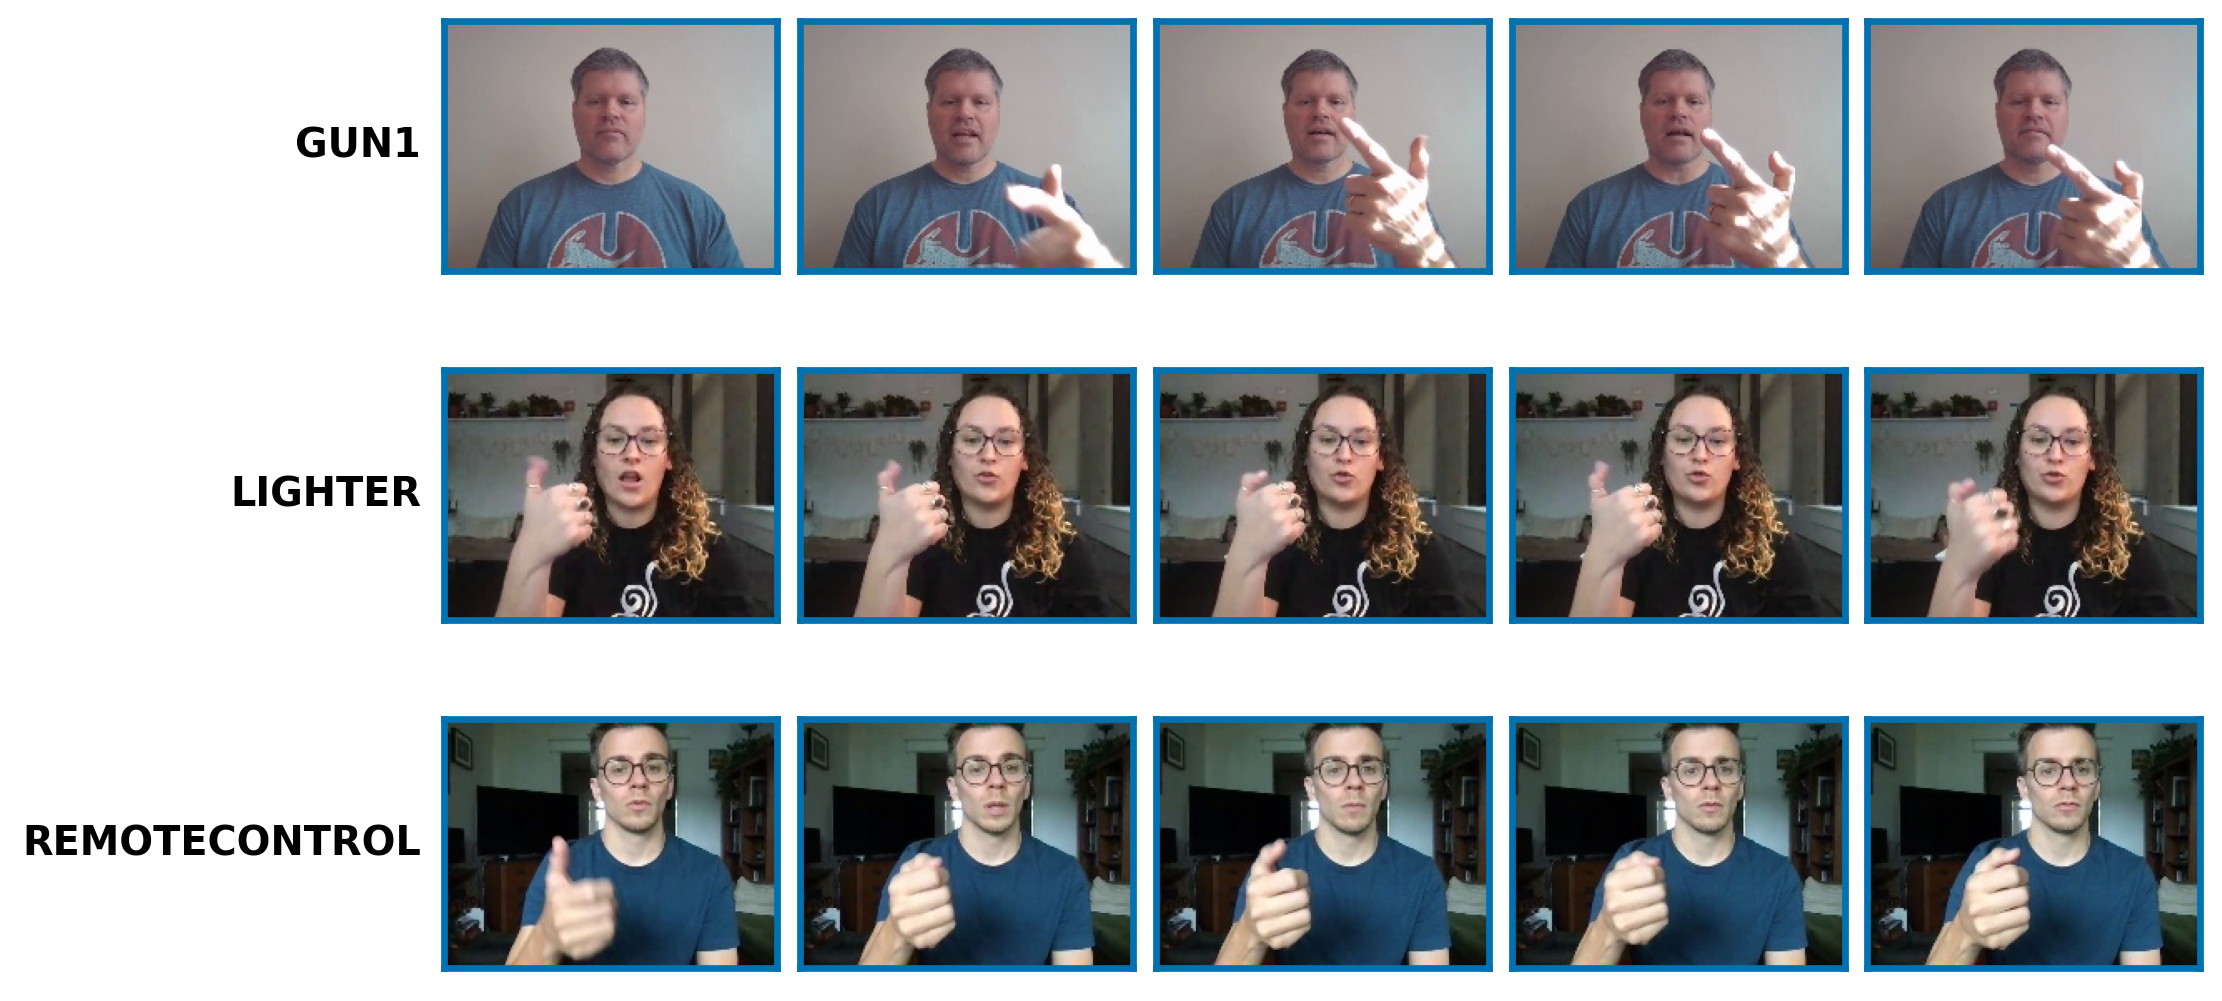
\includegraphics[width=\linewidth]{iconicity_family_example.png}
\caption[A high-iconicity form family]{Same hands, same movement, same
location, different words: GUN1, LIGHTER and REMOTECONTROL share all
five ASL-LEX form features and rate $5.3$--$5.6$ of $7$ on deaf-signer
iconicity.}
\label{fig:iconicity_family}
\end{figure}

We quantify this with a \emph{form-dose} measure: bucket every pair of
gloss centroids by how many of the five features the two glosses share,
and trace cosine similarity against that count. Four things follow, and
together they say where form organisation should come from.

\emph{It is built by pretraining, and it travels.} The frozen backbone
responds strongly on its own: mean centroid similarity climbs from
$0.01$ at zero shared features to $0.18$ at five (Spearman $\rho=.06$).
Logos never trained on ASL Citizen, so this structure has crossed to
another language, another set of signers and another recording setup. It
is also what the Logos authors credit for the quality of their encoder,
and on this benchmark the untouched frozen backbone still beats every
published system (Table~\ref{tab:backbone_ft_retrieval}).

\emph{In-domain training moves it, and the objective decides which way.}
Fine-tuning the backbone on gloss labels flattens the response, plain
cross-entropy most of all ($0.09$ at five shared features, $\rho=.00$):
the model reorganises around whatever separates this particular
vocabulary and gives up the phonological structure it started with. SDDA
is the one intervention that meaningfully protects it, keeping about half
the frozen slope ($0.13$, $\rho=.03$), while aug-as-data and the
consistency pull sit level with plain cross-entropy.
Figure~\ref{fig:form_dose_rho} shows the pattern across every space we
trained: the SignCLIP heads stay near the frozen level on frozen
features, and inherit the flattening when built on a fine-tuned backbone.

\emph{Pushing appearance invariance hard drives it back up, without
being asked to.} The pair-SupCon heads are the only spaces above the
frozen level ($0.25$ at $K{=}3$, $\rho=.09$; $0.39$ at $K{=}5$,
$\rho=.16$), and they see no gloss labels at all: their positives are the
$K$ views of one source video, and every other clip is a negative, two
GUN1 recordings included (\S\ref{sec:method-objectives}). Nothing tells
them which clips share a word. Collapsing appearance variation simply
removes the axis the space was mostly using, and form is what is left to
organise it, so form-similar glosses drift together as a side effect.

\emph{Overshooting the pretrained level is what costs performance.}
Retrieval falls as $K$ rises, from $0.800$ V2T R@1 for the same edits
used as ordinary training data to $0.567$ at $K{=}3$ and $0.414$ at
$K{=}5$: the space collapses the very contrasts the task must tell apart.
The opposite error is harder to see here, because plain cross-entropy
flattens the response furthest and still scores best on this benchmark
($+2.4$ R@1 over frozen), so on retrieval alone the loss looks free.
Retrieval is not the only readout of those features, though. A linear
classifier on the frozen features reaches $86.33$ R@1, the best probe
score in the table, and no fine-tuned space improves on it. The frozen
geometry is therefore not arranged for nearest-neighbour retrieval, which
is why fine-tuning lifts that score, but the class structure is already
there and linearly separable: fine-tuning rearranges the space to suit
the retrieval metric more than it adds information.
A second reason comes from the Logos paper itself. Its authors
report that co-training on all three of their corpora transfers better to
a low-resource target than fine-tuning their RSL-only model on that same
target ($66.82$ against $65.57$ on WLASL), and account for it only by the
higher accuracy reached~\cite{ovodovLogosWellTemperedPretrain2025}.
Flattening offers a mechanism they never test: fine-tuning on one target
gives up the form structure the pretraining built, whereas co-training
keeps the source objective, and with it that structure, alive.
\S\ref{sec:discussion-regimes} develops this. It stays a conjecture,
because the intermediate checkpoints needed to test it are not public.

\begin{figure*}[t]
\centering
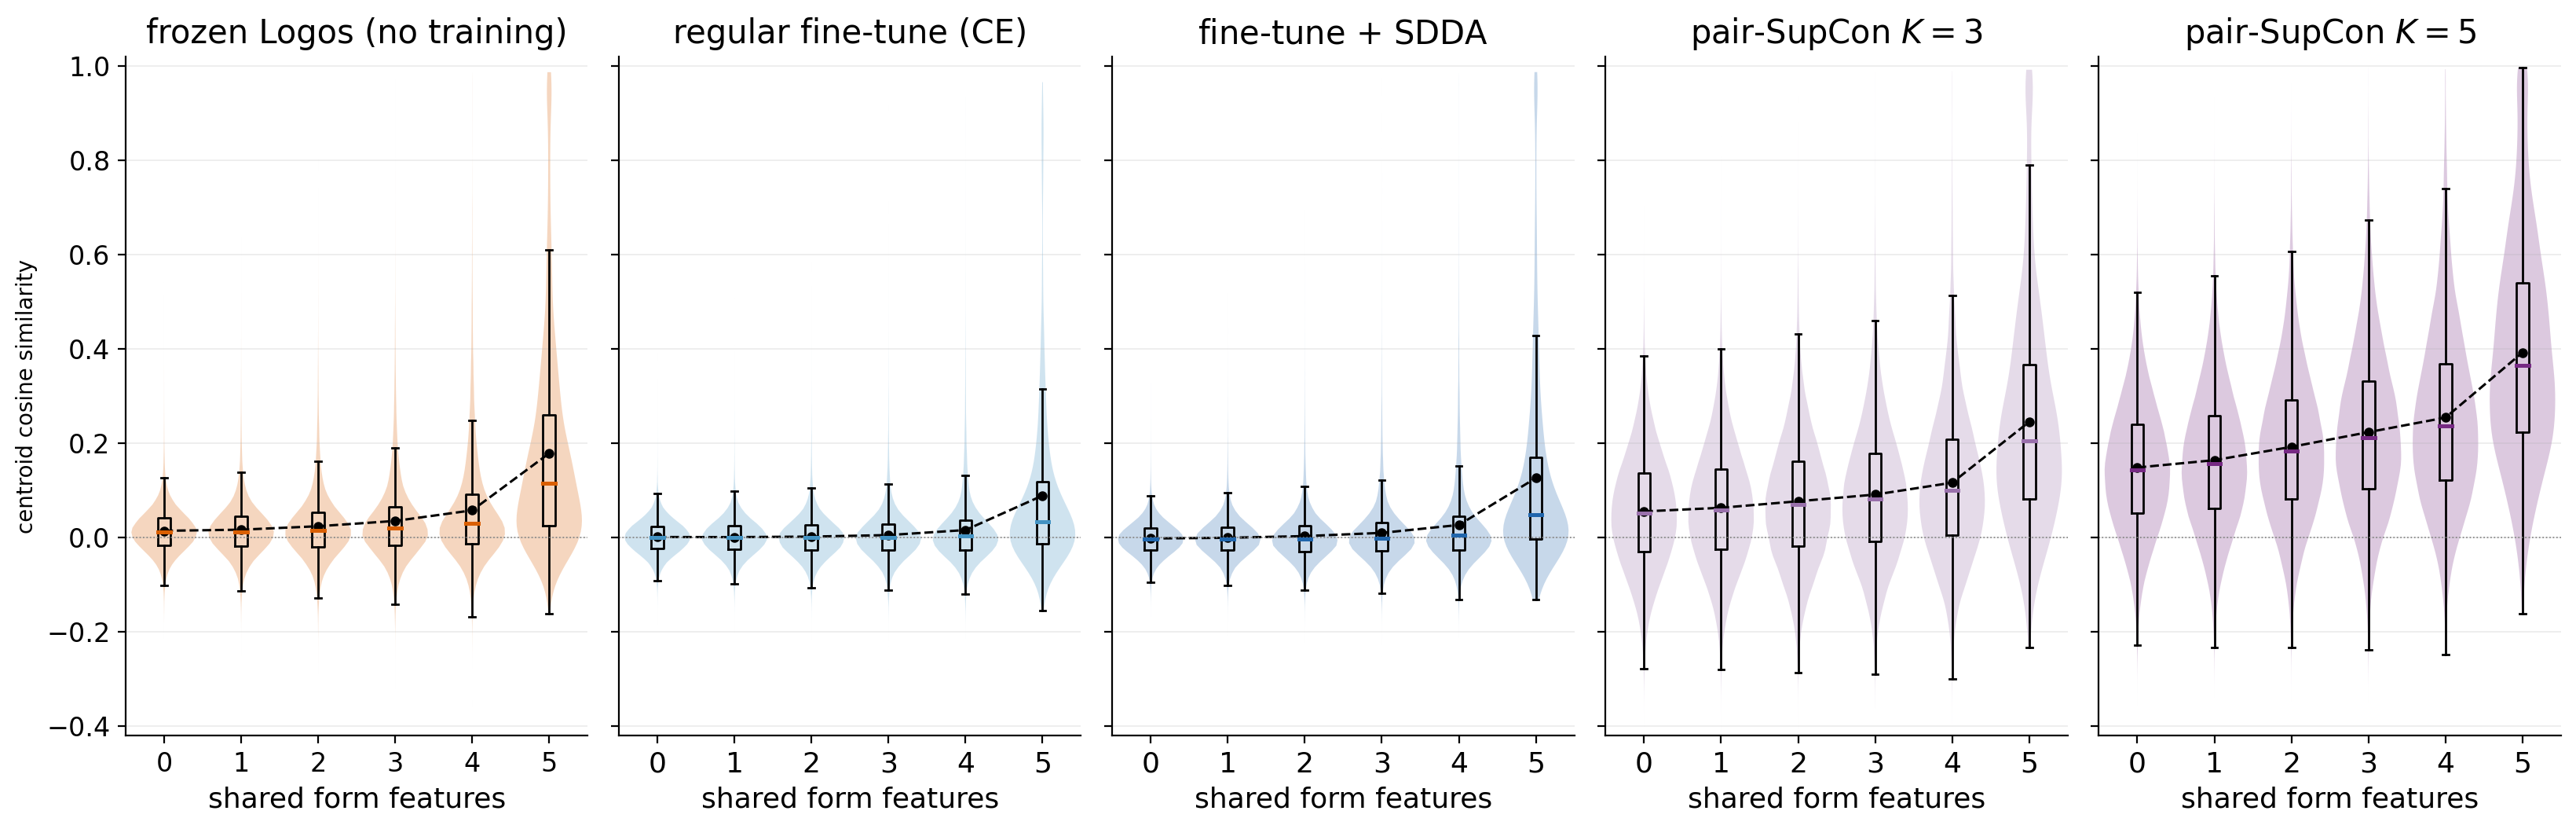
\includegraphics[width=\textwidth]{form_dose_main.png}
\caption[Form-dose response across training recipes]{Centroid cosine
similarity against the number of shared ASL-LEX form features. Boxes are
quartiles, the dashed line the bucket mean. The frozen backbone sits between two opposite
pressures: fine-tuning the backbone flattens the response, most
completely with plain cross-entropy, while training a head with the
appearance counterfactuals as explicit positives amplifies it beyond
the frozen level and increasingly so with $K$. The pair-SupCon panels
also start higher at zero shared features, so the claim concerns the
slope rather than the absolute level. Mean centroid similarity at five
shared features: $0.18$ frozen, $0.09$ CE, $0.13$ SDDA, $0.25$ at
$K{=}3$, $0.39$ at $K{=}5$; the six buckets hold $546{,}736$ to
$2{,}178$ centroid pairs, from zero to five shared features.}
\label{fig:form_dose_ft}
\end{figure*}

\begin{figure}[t]
\centering
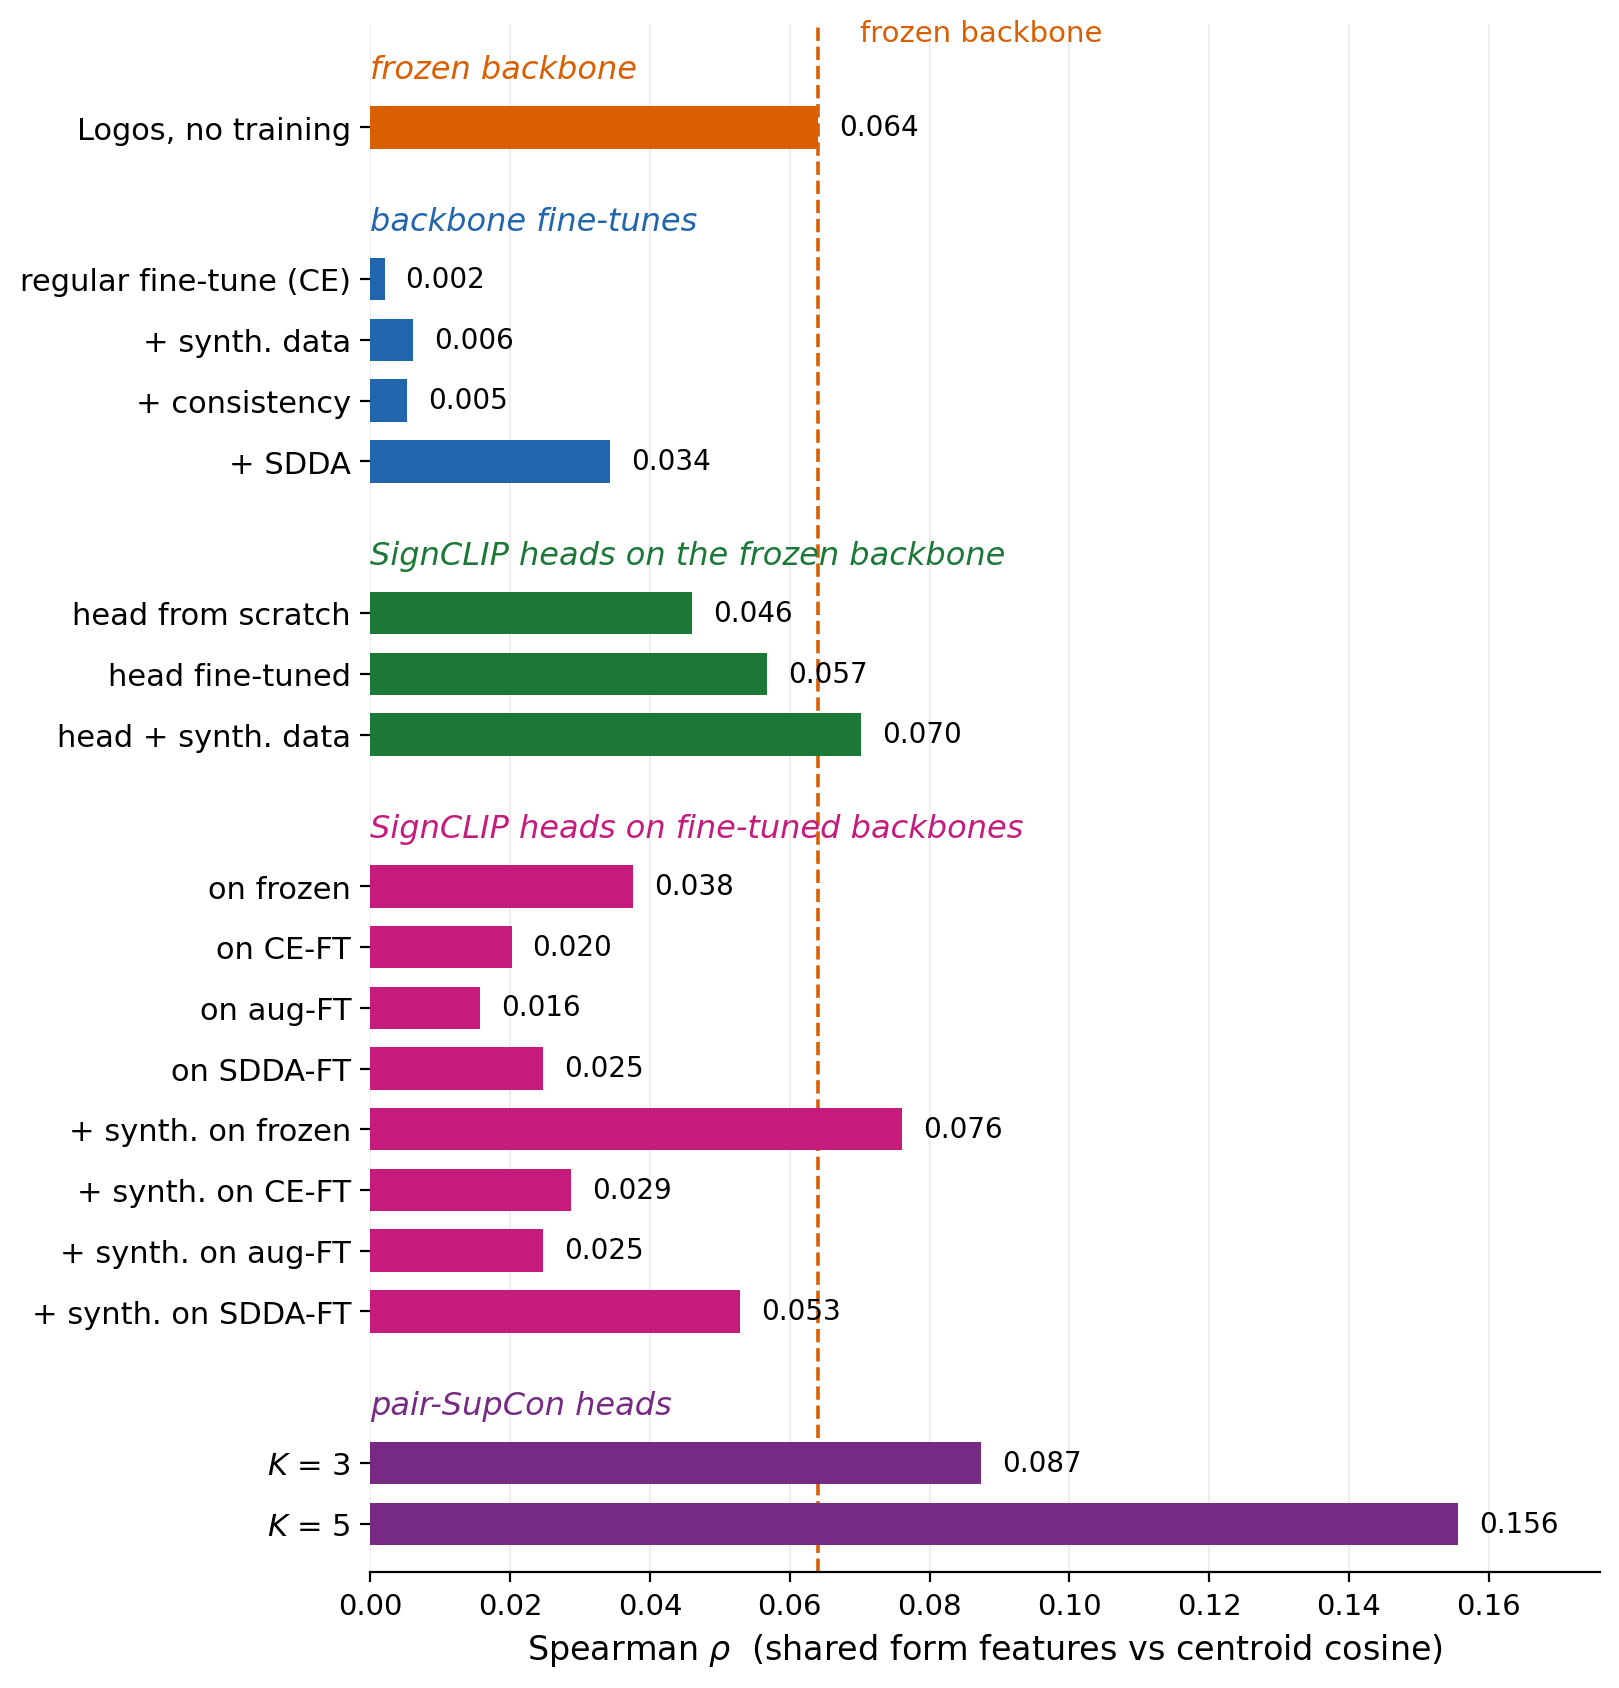
\includegraphics[width=\linewidth]{form_dose_rho.png}
\caption[Form organisation across every trained space]{Form organisation
of every space we trained, as the Spearman correlation between shared
form features and centroid cosine over all gloss pairs. The dashed line
is the frozen backbone. Every backbone fine-tune falls below it, heads
trained on frozen features stay near it, heads on fine-tuned backbones
inherit the flattening, and only the pair-SupCon heads, the ones trained
with the appearance counterfactuals as explicit positives, rise above
it.}
\label{fig:form_dose_rho}
\end{figure}


        \chapter{Discussion}
\label{chap:discussion}

\section{Two regimes, two answers}
\label{sec:discussion-regimes}
Our central empirical pattern is a contrast between regimes. In the high-diversity regime, on
ASL Citizen~\cite{aslcitizen}, the appearance interventions returned a null: no
objective family beats plain cross-entropy at matched depth, and the
frozen backbone's linear probe stays the best in
Table~\ref{tab:backbone_ft_retrieval} on every probe metric, so nothing we
trained made the task more accessible than the untouched representation
already made it. In the
low-diversity NGT744 setting, where the model must bridge a real signer gap from a
handful of recordings, motion-locked synthetic counterfactuals produced
a clear gain. The simplest reading is that appearance invariance is not a
property a model has or lacks in the abstract; it is relative to the
diversity already present in training. The Logos checkpoint we
use~\cite{ovodovLogosWellTemperedPretrain2025} is trained jointly on three
isolated-sign corpora (Logos, AUTSL, and WLASL); the Logos dataset alone
contributes roughly $200{,}000$ videos from $381$ signers, and AUTSL and
WLASL add $43$ and $119$ more.
\todome{REWRITTEN 12.08: the previous sentence attributed the contrast to
backbone pretraining exposure, but both regimes run on the same frozen
checkpoint, so pretraining cannot be the variable that separates them.
Signer counts moved to a consistent whole-corpus basis (was 305 train-split
Logos signers plus a wrong 36 for AUTSL; 43 per the ChaLearn description
in Related Work).}
Both regimes run on this same frozen checkpoint, so pretraining exposure
is a constant across the contrast, not the variable; what differs is the
training data each intervention enters. The ASL Citizen runs already see
$35$ real signers recorded under varied webcam conditions, so the edits
add appearance variation of a kind the split carries anyway. The NGT744
encoder trains on four signers in one studio, and there the synthetic
signers supply appearance diversity the training data otherwise lacks.

% Signer counts, whole-corpus basis (12.08): Logos paper §3.1 gives
% 199,668 videos / 381 signers; AUTSL 43 (ChaLearn, Related Work §2);
% WLASL 119. The paper prints no train-split signer integer, so the
% earlier ~305 train-only estimate was dropped.

A second factor compounds this signer-diversity gap for the raw, untrained
backbone specifically. That Logos transfers well onto ASL Citizen even
before any ASL-Citizen-specific training
(Table~\ref{tab:backbone_ft_retrieval}: the unmodified frozen backbone
already exceeds the benchmark's published baselines with no target-corpus
training at all)
makes sense once the pretraining recipe is considered: Logos is trained
jointly with WLASL, and WLASL and ASL Citizen share a large fraction of
their vocabulary: both are American Sign Language isolated-sign corpora
drawn from an overlapping sign inventory, so the backbone has effectively
already seen much of what ASL Citizen asks of it. The shift to NGT744 removes
that overlap on three axes at once: NGT744 is in a different sign
language entirely (Dutch Sign Language rather than American), its
recordings come from a different capture setup (signers in motion-capture
suits in a studio, rather than webcam video), and its unit of analysis is
sentence-level continuous signing rather than the isolated, gloss-level
clips both ASL Citizen and WLASL provide. Any one of these differences
would weaken transfer; together they are a plausible reason why the same
pretrained backbone that carries over to ASL Citizen with no
target-corpus training needs
the full synthetic-appearance intervention to bridge the NGT744 signer gap.

This reading also bears on SDDA's positive
result~\cite{fuSignerDiversitydrivenData2024b} on PHOENIX-2014T, with a
caveat that has to come first: SDDA reports sign language translation on
continuous video where we report isolated-sign retrieval, so what follows
compares regimes, not two measurements of the same quantity. Their
generatively augmented contrastive setup operates on a studio-recorded corpus
with far less signer variety than ASL Citizen (PHOENIX-2014T contains nine signers in
total~\cite{fuSignerDiversitydrivenData2024b}), i.e.\ closer to our NGT744
% Nine signers verified 2026-07-12 in three independent sources: Camgoz et
% al. 2018 §4 (primary; no bib entry yet — optional to add), the SDDA paper
% itself ("includes data from only nine different signers"), and the Isharah
% paper's comparison table. Cited to SDDA since it is already in the bib and
% is the paper whose corpus is being discussed.
regime than to our ASL Citizen regime.

In PHOENIX-2014T, recording conditions are held fixed (one studio, one camera
setup, one weather-forecast register), so the shift their augmentation has
to bridge is signer appearance and signing style alone, narrower than the
corpus and viewpoint changes our NGT744 evaluation layers on top of it. How
much the held-out-signer choice matters on this corpus is documented
independently: under a full signer-disjoint re-evaluation of
PHOENIX-2014T, mean translation scores fall by between a third and four
fifths depending on the system, and the choice of held-out signer moves
BLEU-4 by up to a factor of ${\sim}5$ for the most affected
one~\cite{artiagaRethinkingSignLanguage2025}.
\section{RGB versus pose, revisited}
\label{sec:discussion-rgb-pose}
Pose input is widely adopted in SLR partly \emph{because} it is assumed
to discard appearance: the robustness of pose-based models is
attributed to inherent invariance to clothing, background and
lighting~\cite{moryossefEvaluatingImmediateApplicability2021,
kratimenosIndependentSignLanguage2020, tranRegionAwarePoseModeling2025},
% keys as used at lines 423-424
and the SignEval organisers went as far as distributing
\emph{only} pose features for a signer-independent task, citing signer
overfitting and privacy~\cite{luqmanSignEval2025Challenge2025a,
alyamiIsharahLargeScaleMultiScene2026b}. % keys as used at lines 182-183
Our diagnostic probes complicate the premise behind both moves. On ASL
Citizen, mean-pooled MediaPipe keypoints are the \emph{most}
signer-separable of the three raw feature spaces we test, on both
readouts: their inter/intra distance ratio is
$29.9\times$ [$28.4$, $32.0$] % table line 1360 (tab:raw_feature_l2_probe)
against
$22.7\times$ and $22.2\times$ % lines 1361-1362 (Logos, I3D)
for the two RGB backbones (confidence intervals overlapping
neither's), % prose lines 1372-1374
and a linear head recovers the signer at
$98.7\%$ % line 1360 (MediaPipe decoding; chance 3.0%, caption line 1354
% and prose lines 1370-1371)
against $94.2\%$ (I3D) and $65.9\%$ (Logos), an ordering unchanged on
the signer-disjoint test split
($99.4\%$/$95.2\%$/$74.3\%$, chance $9.1\%$). % lines 1374-1376
One asymmetry bounds the reading: the two RGB spaces come from
gloss-supervised backbones, which \S\ref{sec:results-l2-raw} shows sheds
linearly accessible identity, while the keypoints are untrained
coordinates, so the ordering measures what pose \emph{retains}, not what
the modality would concentrate at matched training.
Camera framing cannot carry this: the keypoints are root-centred at the
shoulder midpoint and scale-normalised to shoulder width, so what
identifies the signer is shoulder-normalised geometry: body
proportions, habitual posture, movement style. % prose lines 1376-1381
Nor is it gloss content in disguise: under gloss-disjoint
cross-validation on ASL Citizen, where the classifier is tested only on
signs no signer contributed during its training, the decoding numbers
are essentially unchanged ($98.7\%$/$94.6\%$/$64.5\%$,
\S\ref{sec:results-l2-raw}).
Pose discards pixels; on this evidence it retains precisely the
person-specific signal the modality is assumed to remove.

This lands on the same side as the fairness literature reviewed in
\S\ref{sec:related-work-modality}, from the opposite direction. That literature's caveat is about
the \emph{extractor}: pose pipelines are themselves learned RGB models
whose training and evaluation sets under-represent darker-skinned
individuals~\cite{lachanceCaseStudyFairness2023,
hasanHi5SyntheticData2024}, % keys as used at line 194
whose audits reach conclusions that flip with the evaluation
set~\cite{lachanceCaseStudyFairness2023,
xiangFairHumanCentricImage2025}, % keys as used at line 203
whose hand tracking degrades exactly where signing is linguistically
dense~\cite{moryossefOptimizingHandRegion2024,
moryossefEvaluatingImmediateApplicability2021}, % keys as used at lines 218-221
and whose ASL Citizen pose baseline shows larger skin-tone and gender
disparities than its RGB
counterpart~\cite{atwellStudyingMitigatingBiases2024}. % key as used at line 210
Our probes add the complementary caveat about the \emph{representation}:
even when extraction succeeds and coordinates are normalised, the
resulting features are more signer-identifying than either RGB space we
compare against. Together the two caveats suggest that treating pose
distribution as an appearance-bias or privacy fix (as in the
pose-only challenge protocol above) deserves the same scrutiny as
any other debiasing claim: the appearance axis a pose skeleton removes
(clothing, background, skin pixels) is not the only axis along which
signers are identifiable, and by our measurements not the dominant one.

The scope of this claim should be stated as narrowly as the evidence.
Ours is a bias probe, not a matched-capacity recognition comparison: we
never train a pose-based recogniser ourselves (the pose rows of
Table~\ref{tab:asl_citizen_retrieval} are the published results of the
original SignCLIP model), % setup lines 1058-1061
so we make no claim about whether pose-based \emph{models} exploit this
identity signal, how much it costs them under signer shift, or how the
modalities compare at matched training: questions the recent
RGB-versus-pose results
cited in \S\ref{sec:related-work-modality}~\cite{minCloserLookSkeletonbased2025,
wongSignRepEnhancingSelfSupervised2025} % keys as used at lines 419, 240
address from the accuracy side. 
What the probes do establish is the narrower, assumption-level point:
signer identity is not removed by pose extraction by construction, and
a pipeline that adopts pose \emph{for} invariance or privacy inherits
an unexamined assumption rather than a guarantee.

\todome{REWRITTEN 12.08: the previous version compared the heads'
train-split $\rho$ against the test-split reference ($17.67\times$),
which the table caption itself forbids; against the train-split frozen
ratio the geometric half of the claim disappears. The matching caption
fix resolves the `framing check' todo that sat on
tab:head\_signer\_probes.}
After training, the two readouts come apart. The SignCLIP-style heads
make identity far \emph{less} linearly decodable ($20$--$25\%$ against
$66.9\%$ for the frozen features on the same split, chance $2.9\%$)
while leaving the distance geometry near the frozen level
($22.0$--$23.4\times$ against $22.7\times$,
Table~\ref{tab:raw_feature_l2_probe}), with only the $K{=}5$ pair-SupCon
head clearly above it ($26.3\times$,
Table~\ref{tab:head_signer_probes}). By the bar set in
\S\ref{sec:results-ft-probes}, that an intervention which genuinely
removes identity must lower both readouts, no objective in this thesis
removed signer structure; training moved where that structure is
measurable, which is the reason to report both probes rather than treat
linear decodability as \emph{the} appearance-bias metric.

\section{Limitations}
\label{sec:limitations}

\textbf{Untrimmed NGT744 recordings.} The NGT744 training videos were not
trimmed: each begins with a lengthy idle segment in which the signer
stands watching the reference video before starting to sign, and ends
with a reach toward the foot pedal used to stop the recording. Both add
frames unrelated to signing (idle standing and extraneous motion),
and because the idle portion differs in length per signer, no trivial
automated trim existed; we judged manual cleaning not worth thesis time.

\textbf{Frame-independent generative editing introduces flicker.} Our
editing pipeline (\S\ref{subsection:GAE}) edits each frame of a
source video independently: every edited frame follows the appearance-edit
prompt on its own, with no explicit mechanism enforcing consistency with
the frame before or after it, so consecutive edited frames drift slightly
relative to one another and the resulting clip flickers. We looked for a
video-native alternative that would edit a clip as one temporally
consistent unit rather than frame-by-frame, trying LTX 2.3 (22B)
~\cite{hacohen2026ltx2}, LTX 2.3 with an Edit Anything
LoRA~\cite{alissonerdx2026editanything}, Wan
2.2~\cite{wan2025}, and Lucy Edit 1.1 dev
(5B)~\cite{decart2025lucyedit};
in every case the edited
output was, on visual inspection, substantially worse than the
frame-by-frame FLUX.2-klein-9B route, so we
kept the per-frame pipeline and report the resulting flicker as a
limitation rather than a solved problem.

\textbf{Occasional generative hallucinations.} The editing model
occasionally hallucinates content that was not in the source frame:
most visibly, adding a spurious or malformed handshape to a frame whose
original signer was not making that shape, or to a frame that did not
contain a visible hand at all. This risk is highest for the skin-tone and
signer-swap edit types (\S\ref{subsection:GAE}), and is a direct
consequence of editing each frame independently rather than conditioning
on the sign actually being performed.
 A more heavily
constrained editing pipeline (for instance, conditioning the editor
on the source pose via ControlNet-style
conditioning~\cite{zhangAddingConditionalControl2023}) could reduce these hallucinations
further; we did not quantify their prevalence, and judged the added
pipeline complexity out of scope for this thesis.

\todome{ADDED 12.08: experiment-level limitations; the previous three
items covered only the generation tooling. Cut whatever you disagree
with.}
\textbf{Statistical and coverage limits of the ASL Citizen experiments.}
Every ASL Citizen cell is a single training run, without seeds or
confidence intervals, against a nuisance floor that is not zero (probe
retest spread up to $1.8$ points; a $1.8$-point retrieval shift from a
change of frame preprocessing alone); the NGT744 experiments carry three
seeds and per-seed significance tests, the ASL Citizen ones do not. The
generative edits reach $450$ of the $2{,}731$ glosses ($14.9\%$ of
training videos), and the corpus's minimum of eight signers per gloss
bounds the headroom any signer-diversity intervention can have there
(\S\ref{sec:setup-generation}). Finally, the two regimes differ in more
than signer diversity: sign language, capture setup and unit of analysis
all change between ASL Citizen and NGT744
(\S\ref{sec:discussion-regimes}), and the from-scratch control that
would isolate the diversity account remains future work
(\S\ref{sec:future-work}).

\section{Future work}
\label{sec:future-work}
\textbf{Recovering motion from video rather than from motion capture.}
The motion-locked route requires motion-capture recordings, which is why
it could not be applied to a corpus that provides only RGB video
(\S\ref{sec:method-diffusion}). Estimating parametric
SMPL-X~\cite{pavlakosExpressiveBodyCapture2019a} pose and shape from the
video itself would replace that input, so that the recovered parameters
drive the same rendering and the route extends to any corpus.
SignAvatars~\cite{yuSignAvatarsLargeScale3D2025} and Neural Sign
Actors~\cite{baltatzisNeuralSignActors2024a} show what such
parametrisation looks like for signing, though both would need to improve
substantially before they could stand in for recorded capture.

\textbf{Signer identity persists through the synthetic-avatar swap.}
Even
when signer identity is changed by re-rendering with a synthetic avatar,
the avatar does not fully erase who provided the underlying motion
capture: body shape, body posture, range of motion when signing, and
signing speed are all retargeted along with the sign itself, and all four
remain visibly present in the render. This is consistent with the
diagnosis that shoulder-normalised body geometry and movement style
identify signers (\S\ref{sec:results-diagnosis}), and it is plainly
visible: an observer with no knowledge of sign language can still tell,
from individual frames of the renders, which real NGT744 signer supplied
the motion capture for a given avatar. The synthetic-signer
intervention changes surface appearance (body model, clothing, skin
tone) without fully removing the motion-level signature of the source
signer, a distinction the retrieval-based evaluation in this thesis does
not separate out. Measuring that motion-level signature directly (a
signer-identity probe on the rendered views themselves) would be a
cheap first step, and motion retargeting that also perturbs kinematic
style the harder follow-up.

\textbf{Augmenting the full ASL Citizen training set, not just a targeted
subset.} Our generative augmentation covers a deliberately targeted subset
of the ASL Citizen training set, chosen worst-first by signer scarcity and
baseline difficulty (\S\ref{sec:method-diffusion}). The subset itself was
set by the generation compute budget (\S\ref{sec:setup-generation});
evidence that targeted synthetic augmentation can outperform augmenting
everything~\cite{nguyenDoWeNeedSynthetic2025} guided how the subset was
chosen, not whether to use one.
Whether that finding transfers to our setting is untested: it remains an
open question whether augmenting the entire training set, rather than the
selected worst-first subset, would have produced a larger gain
than the targeted budget did, or whether the targeted-subset advantage
holds here too and full-corpus augmentation would mostly add compute cost
without adding retrieval gain.

\textbf{End-to-end training for the NGT744 encoder.} All NGT744 results come
from an encoder trained on pre-extracted, frozen Logos clip features
(\S\ref{sec:results-lowdiv}). An end-to-end variant that prepends
the MViTv2-S backbone itself (a frozen-backbone control and a fully
fine-tuned configuration) was implemented and configured but never
run. Running both would show whether the low-diversity gain from
synthetic views survives, grows, or shrinks once gradients can reach the
visual backbone, giving the low-data regime its own counterpart to the
contrast between frozen-feature heads and backbone
fine-tuning (\S\ref{sec:discussion-regimes}).

\textbf{A discriminative term for the high-$K$ arms.} Packing more
synthetic views into a training item does not pay: on NGT744, stacking
side-view renders onto the matched arm drops R@1 from $0.649$ to $0.437$
(E3 to E5), adding further generative edits drifts it from $0.505$ to
$0.461$ (E4 to E7), and the pair-SupCon head points the same way on ASL
Citizen ($0.567$ at $K{=}3$ falling to $0.414$ at $K{=}5$). Schedules are
matched to each arm's update count and the contrastive batch is fixed at
$64$ items for every arm (\S\ref{sec:setup-training}), so neither
truncated training nor negative starvation accounts for the drops. Our
reading is that pure SupCon at high $K$ spends its capacity making views
of the same item indistinguishable, at the cost of keeping different
items apart. A
natural test is to add a discriminative term to the NGT744 training setup
(a 12-layer encoder trained with SupCon on frozen Logos clip features;
\S\ref{sec:results-lowdiv}): cross-entropy on sentence-recording
identity plus $\lambda$ times the SupCon term, sweeping
$\lambda \in \{0.1, 1\}$ over a subset of arms. If the high-$K$ drop
disappears, the tradeoff is objective-specific and fixable; if it
persists, appearance invariance itself is what costs retrieval.

\textbf{A from-scratch control for the high-diversity null.} The two-regime
reading attributes the flat high-diversity result to appearance
invariance already supplied by real diversity, in pretraining and in the
35-signer training split (\S\ref{sec:discussion-regimes}), and the
pretraining half of this
is directly testable: train the same MViTv2-S from random initialisation
on ASL Citizen, with cross-entropy alone and with the synthetic
augmentations added, and compare against the pretrained baseline. If the
from-scratch model lands well below the pretrained one and the
augmentations now help it, pretraining diversity, not a saturated
recipe, explains the null; if augmentation still adds nothing, the
ceiling is not a pretraining artifact. 

\textbf{Fine-tuning I3D as a second backbone for the embedding-space
analyses.} Throughout this thesis I3D is used only as a frozen,
off-the-shelf feature extractor (\S\ref{sec:results-diagnosis},
\S\ref{sec:results-highdiv}), never fine-tuned the way the Logos/MViTv2-S
backbone is. Repeating the fine-tuning runs and the embedding-space
analyses (signer-separability probes, form-dose geometry) with a
fine-tuned I3D would show whether this thesis's diagnostic findings are
specific to the MViTv2-S/Logos backbone or hold across RGB architectures
more generally.

        \chapter{Conclusion}
\todome{DRAFT START (Claude 04.08): conclusion chapter, five paragraphs --- restate, diagnosis, NGT, ASL Citizen, two-regime takeaway + outlook; no numbers beyond those already in the body}
This thesis asked whether sign language recognition models lean on the
incidental appearance of the recorded signers (clothing, skin tone,
body shape, environment) rather than the signing itself, and whether
synthetic appearance counterfactuals, edited copies of training videos in
which appearance changes while the performed sign is preserved, can
remove that bias. We pursued the question through one diagnosis and two
interventions: motion-locked avatar re-renders of a
self-recorded NGT744 corpus, where the counterfactual property holds by
construction, and generative per-frame appearance edits of ASL
Citizen videos, the scalable approximation of the same idea at benchmark
scale.
% Restatement condenses the abstract (lines 76-88) and the introduction's
% pipeline framing (lines 247-265); "by construction" vs "approximation,
% not a substitute" from lines 251-252 and 262-265.

The diagnosis came back positive everywhere we looked. Signer identity is
recoverable from every feature space we test, including pose-based ones:
on ASL Citizen the raw spaces separate signers at fixed sign content by a
distance ratio of $22$--$30\times$, and a linear head recovers the signer
far above chance in all three spaces, with the MediaPipe pose features,
often adopted precisely to escape appearance, the most
signer-separable of all, at $98.7\%$ decoding accuracy.
% "recoverable from every feature space we test, including pose-based
% ones" from the abstract, lines 82-84; "$22$--$30\times$" and "a linear
% head recovers the signer far above both chance ... in all three spaces"
% from lines 1355-1359; "98.7%" from line 1348/1361; "most signer-separable"
% from lines 1359-1360.

The two interventions returned two different answers. In the
low-diversity NGT744 setting (four training signers, one studio
environment at train time), synthetic signers more than double
cross-signer retrieval (R@1 $0.23 \to 0.65$ test$\to$train; $0.25 \to
0.70$ train$\to$test, 3 seeds), a gain that a real-multiview control at
the same view count does not reproduce: appearance and identity
diversity, not extra viewpoints, is what drives it. At matched view
count, content, and viewpoint, the generative edits retain roughly
$65$--$80\%$ of the avatar gain, and as real signer diversity is added
at a fixed data budget, the full-strength synthetic gain shrinks,
consistent with synthetic appearance variety substituting for real
diversity that is absent.
% NGT headline numbers and "more than double" from the abstract, lines
% 89-91; multiview control from lines 1525-1534; "65--80%" from lines
% 1518-1520; the shrinking full-Unreal gain (+0.145 -> +0.081 test->train)
% from lines 1611-1614 and fig:ngt_dropoff (lines 1698-1707); "substitutes
% for absent real diversity" phrasing from the fig caption, lines
% 1704-1706. NOTE: the matched-K panel's gain does NOT shrink (lines
% 1615-1621) --- I kept the claim scoped to "full-strength" to stay
% accurate; do not generalise it.

On the large, signer-diverse ASL Citizen benchmark the same idea leaves
recognition essentially unchanged across every objective family we try
(augmentation-as-data, cosine consistency, supervised contrast, and
adversarial invariance), with one modest exception: adding the
counterfactuals to a frozen-feature contrastive head is worth $+1.1$
R@1, while backbone fine-tuning gains nothing over plain cross-entropy.
% "essentially unchanged" + family list from the abstract, lines 93-95;
% "+1.1 R@1 on a frozen-feature head, nothing at the backbone" from line
% 2423; "No appearance or signer-invariance objective beats plain
% cross-entropy at matched depth" from lines 1778-1780.
The embedding-space analyses explain what the retrieval numbers alone
cannot. The counterfactuals themselves are faithful: local edits move an
embedding about half as far as a genuine signer change, the signer swap
exactly as far as one, and although the augments are near-perfectly
linearly separable from real video, that entire linear signature
collapses to a single shared offset per edit type, a direction a
classifier can trivially factor out.
% n.disp 0.44--0.53 local / 1.04--1.05 swap paraphrased from lines
% 2286-2290; "near-perfectly linearly separable" (AUC 0.96--1.00) from
% lines 2305-2310; de-shift collapse to chance (0.48--0.51) and "a
% direction a classifier can trivially factor out" from lines 2311-2323.
And the invariance objectives are not inert: fine-tuning measurably
erodes the linearly decodable component of signer identity,
consistency training most of all, yet that erosion does not translate
into better retrieval, so removing decodable signer information and
improving retrieval accuracy are dissociable outcomes here.
% Decoding erosion (75.3% frozen -> 64.2% CE -> 56.3% consistency) and
% "does not translate into better retrieval ... dissociable outcomes"
% from lines 2092-2105.

The two regimes together give the thesis its answer. Appearance
invariance is not a property a model has or lacks in the abstract; it is
relative to the diversity already present in training. Where real signer
diversity is scarce, as in our four-signer NGT744 corpus and the
few-signer studio corpora of prior positive results, synthetic
appearance counterfactuals earn their cost, and motion-locked
re-renders earn the most; where hundreds of pretraining signers and diverse
recording conditions have already bought the invariance, the same
counterfactuals are largely redundant.
% "not a property a model has or lacks in the abstract; it is relative to
% the diversity already present in training" from lines 2426-2428; the
% prior-positive-results clause refers to the SDDA/PHOENIX comparison
% (nine signers total, five in training), lines 2462-2502; "earn their
% cost ... largely redundant" from the abstract, lines 97-99.
The most direct continuations follow the same axis: parametric avatars
that turn appearance into a sampled variable rather than an authored
asset, a dose-response sweep over the number of synthetic signers, and a
from-scratch control that would test directly whether pretraining
diversity is what consumed the gain in the high-diversity regime.
% Outlook items are the existing future-work themes only: SMPL-X
% parametric avatars (lines 2595-2606), scaling laws / dose-response
% (lines 2608-2611), from-scratch control (lines 2677-2686).
\todome{DRAFT END: (i) no new numbers or claims --- every figure is quoted
from the abstract/results/discussion with line refs in the comments;
(ii) para 3 deliberately scopes the shrinking-gain claim to the
full-strength arm because the matched-$K$ gain stays flat (lines
1615-1621); (iii) para 5's "prior positive results" clause leans on the
SDDA regime comparison in the Discussion --- if you cut or reframe that
section, soften the clause; (iv) I did not cite the pose-diagnosis
implications for the RGB-vs-pose debate here since the Discussion section
for it (line 2533) is still an unresolved todo; (v) the NGT numbers
include the untrimmed-recording noise floor per the Limitations (lines
2542-2549) --- I left that caveat out of the conclusion as the chapter
already owns it, but flag if you want one hedging clause.}


\bibliographystyle{ACM-Reference-Format}
\bibliography{bibliographies/bibentries}

% Single-column appendix (template: choose one and stick to it)
\onecolumn
\appendix
        \chapter{Appendix}
\section{Full augmentation-geometry grid}
\label{app:aug_geometry_grid}
Tables~\ref{tab:aug_geometry_grid_train} and~\ref{tab:aug_geometry_grid_test} report every cell of the \S\ref{sec:results-aug-geometry} analysis (all five feature spaces $\times$ four edit types $\times$ both evaluation samples) with uncertainty estimates for the quantities the main-text tables report as point values.

\begin{table}[H]
\centering
\footnotesize
\setlength{\tabcolsep}{3.5pt}
\begin{tabular}{lccccc}
\toprule
\textbf{Edit type} & \textbf{n.disp [95\% CI]} & \textbf{AUC} & \textbf{AUC$_{\text{de-shift}}$} & \textbf{gloss@1} & \textbf{flip} \\
\midrule
\multicolumn{6}{l}{\emph{frozen}} \\
\;\;glasses & 0.46 [0.45, 0.48] & 0.993\,$\pm$\,0.001 & 0.50\,$\pm$\,0.00 & 0.58 & 0.67 \\
\;\;shirt & 0.53 [0.52, 0.54] & 0.999\,$\pm$\,0.000 & 0.50\,$\pm$\,0.01 & 0.62 & 0.76 \\
\;\;skin tone & 0.44 [0.43, 0.45] & 0.997\,$\pm$\,0.000 & 0.51\,$\pm$\,0.00 & 0.63 & 0.68 \\
\;\;signer swap & 1.04 [1.03, 1.06] & 1.000\,$\pm$\,0.000 & 0.51\,$\pm$\,0.00 & 0.49 & 0.91 \\
\;\;all edits (pooled) & --- & 0.997\,$\pm$\,0.000 & --- & --- & --- \\
\midrule
\multicolumn{6}{l}{\emph{CE}} \\
\;\;glasses & 0.52 [0.51, 0.54] & 0.983\,$\pm$\,0.002 & 0.50\,$\pm$\,0.01 & 0.67 & 0.66 \\
\;\;shirt & 0.53 [0.52, 0.54] & 0.998\,$\pm$\,0.001 & 0.50\,$\pm$\,0.00 & 0.72 & 0.74 \\
\;\;skin tone & 0.51 [0.50, 0.52] & 0.990\,$\pm$\,0.001 & 0.50\,$\pm$\,0.00 & 0.71 & 0.69 \\
\;\;signer swap & 1.13 [1.12, 1.14] & 1.000\,$\pm$\,0.000 & 0.50\,$\pm$\,0.01 & 0.56 & 0.92 \\
\;\;all edits (pooled) & --- & 0.992\,$\pm$\,0.001 & --- & --- & --- \\
\midrule
\multicolumn{6}{l}{\emph{aug-as-data}} \\
\;\;glasses & 0.59 [0.58, 0.60] & 0.983\,$\pm$\,0.003 & 0.51\,$\pm$\,0.01 & 0.89 & 0.63 \\
\;\;shirt & 0.62 [0.61, 0.63] & 0.998\,$\pm$\,0.001 & 0.51\,$\pm$\,0.00 & 0.92 & 0.67 \\
\;\;skin tone & 0.63 [0.62, 0.64] & 0.992\,$\pm$\,0.001 & 0.51\,$\pm$\,0.01 & 0.90 & 0.68 \\
\;\;signer swap & 1.04 [1.03, 1.05] & 1.000\,$\pm$\,0.000 & 0.51\,$\pm$\,0.00 & 0.91 & 0.80 \\
\;\;all edits (pooled) & --- & 0.991\,$\pm$\,0.002 & --- & --- & --- \\
\midrule
\multicolumn{6}{l}{\emph{consistency}} \\
\;\;glasses & 0.44 [0.43, 0.45] & 0.978\,$\pm$\,0.001 & 0.50\,$\pm$\,0.01 & 0.87 & 0.48 \\
\;\;shirt & 0.41 [0.40, 0.42] & 0.993\,$\pm$\,0.001 & 0.51\,$\pm$\,0.00 & 0.88 & 0.47 \\
\;\;skin tone & 0.44 [0.44, 0.45] & 0.986\,$\pm$\,0.001 & 0.51\,$\pm$\,0.00 & 0.87 & 0.50 \\
\;\;signer swap & 0.79 [0.78, 0.80] & 0.998\,$\pm$\,0.000 & 0.51\,$\pm$\,0.01 & 0.89 & 0.60 \\
\;\;all edits (pooled) & --- & 0.986\,$\pm$\,0.001 & --- & --- & --- \\
\midrule
\multicolumn{6}{l}{\emph{SDDA}} \\
\;\;glasses & 0.37 [0.36, 0.38] & 0.991\,$\pm$\,0.001 & 0.50\,$\pm$\,0.01 & 0.67 & 0.50 \\
\;\;shirt & 0.33 [0.32, 0.34] & 0.998\,$\pm$\,0.000 & 0.50\,$\pm$\,0.00 & 0.72 & 0.51 \\
\;\;skin tone & 0.39 [0.38, 0.39] & 0.997\,$\pm$\,0.000 & 0.51\,$\pm$\,0.00 & 0.70 & 0.52 \\
\;\;signer swap & 0.76 [0.75, 0.78] & 1.000\,$\pm$\,0.000 & 0.50\,$\pm$\,0.01 & 0.67 & 0.67 \\
\;\;all edits (pooled) & --- & 0.996\,$\pm$\,0.000 & --- & --- & --- \\
\bottomrule
\end{tabular}
\caption[Full augmentation-geometry grid, training pairs]{Full augmentation-geometry grid, training pairs ($6{,}000$ per edit type, selection-biased). n.disp = median normalised displacement with the $95\%$ bootstrap confidence interval of the median; AUC and AUC$_{\text{de-shift}}$ = mean $\pm$ sd over the five grouped cross-validation folds; gloss@1 and flip (medians) as defined in \S\ref{sec:results-aug-geometry}. The pooled row is the all-edit-types AUC quoted in Table~\ref{tab:aug_geometry_spaces}.}
\label{tab:aug_geometry_grid_train}
\end{table}

\begin{table}[H]
\centering
\footnotesize
\setlength{\tabcolsep}{3.5pt}
\begin{tabular}{lccccc}
\toprule
\textbf{Edit type} & \textbf{n.disp [95\% CI]} & \textbf{AUC} & \textbf{AUC$_{\text{de-shift}}$} & \textbf{gloss@1} & \textbf{flip} \\
\midrule
\multicolumn{6}{l}{\emph{frozen}} \\
\;\;glasses & 0.50 [0.45, 0.56] & 0.960\,$\pm$\,0.008 & 0.50\,$\pm$\,0.02 & 0.70 & 0.57 \\
\;\;shirt & 0.47 [0.43, 0.51] & 0.990\,$\pm$\,0.003 & 0.50\,$\pm$\,0.01 & 0.75 & 0.56 \\
\;\;skin tone & 0.46 [0.44, 0.48] & 0.972\,$\pm$\,0.007 & 0.50\,$\pm$\,0.02 & 0.74 & 0.54 \\
\;\;signer swap & 1.05 [1.00, 1.10] & 1.000\,$\pm$\,0.000 & 0.50\,$\pm$\,0.02 & 0.59 & 0.77 \\
\;\;all edits (pooled) & --- & 0.976\,$\pm$\,0.003 & --- & --- & --- \\
\midrule
\multicolumn{6}{l}{\emph{CE}} \\
\;\;glasses & 0.48 [0.43, 0.51] & 0.947\,$\pm$\,0.010 & 0.51\,$\pm$\,0.02 & 0.70 & 0.52 \\
\;\;shirt & 0.42 [0.38, 0.44] & 0.993\,$\pm$\,0.002 & 0.50\,$\pm$\,0.02 & 0.77 & 0.54 \\
\;\;skin tone & 0.46 [0.44, 0.50] & 0.968\,$\pm$\,0.012 & 0.49\,$\pm$\,0.02 & 0.75 & 0.55 \\
\;\;signer swap & 1.00 [0.96, 1.05] & 1.000\,$\pm$\,0.000 & 0.50\,$\pm$\,0.03 & 0.60 & 0.76 \\
\;\;all edits (pooled) & --- & 0.972\,$\pm$\,0.005 & --- & --- & --- \\
\midrule
\multicolumn{6}{l}{\emph{aug-as-data}} \\
\;\;glasses & 0.64 [0.59, 0.68] & 0.949\,$\pm$\,0.005 & 0.49\,$\pm$\,0.02 & 0.72 & 0.48 \\
\;\;shirt & 0.58 [0.55, 0.62] & 0.975\,$\pm$\,0.005 & 0.49\,$\pm$\,0.02 & 0.76 & 0.49 \\
\;\;skin tone & 0.66 [0.63, 0.72] & 0.963\,$\pm$\,0.009 & 0.51\,$\pm$\,0.02 & 0.76 & 0.57 \\
\;\;signer swap & 1.17 [1.11, 1.24] & 0.992\,$\pm$\,0.004 & 0.48\,$\pm$\,0.02 & 0.62 & 0.69 \\
\;\;all edits (pooled) & --- & 0.949\,$\pm$\,0.006 & --- & --- & --- \\
\midrule
\multicolumn{6}{l}{\emph{consistency}} \\
\;\;glasses & 0.55 [0.51, 0.61] & 0.946\,$\pm$\,0.009 & 0.48\,$\pm$\,0.02 & 0.67 & 0.43 \\
\;\;shirt & 0.48 [0.44, 0.51] & 0.961\,$\pm$\,0.013 & 0.51\,$\pm$\,0.02 & 0.75 & 0.47 \\
\;\;skin tone & 0.59 [0.54, 0.63] & 0.952\,$\pm$\,0.011 & 0.50\,$\pm$\,0.02 & 0.74 & 0.53 \\
\;\;signer swap & 1.11 [1.05, 1.19] & 0.986\,$\pm$\,0.004 & 0.49\,$\pm$\,0.02 & 0.57 & 0.68 \\
\;\;all edits (pooled) & --- & 0.942\,$\pm$\,0.013 & --- & --- & --- \\
\midrule
\multicolumn{6}{l}{\emph{SDDA}} \\
\;\;glasses & 0.40 [0.36, 0.43] & 0.931\,$\pm$\,0.008 & 0.51\,$\pm$\,0.02 & 0.69 & 0.48 \\
\;\;shirt & 0.31 [0.29, 0.33] & 0.964\,$\pm$\,0.004 & 0.50\,$\pm$\,0.01 & 0.77 & 0.42 \\
\;\;skin tone & 0.40 [0.37, 0.43] & 0.940\,$\pm$\,0.011 & 0.50\,$\pm$\,0.02 & 0.74 & 0.50 \\
\;\;signer swap & 0.80 [0.75, 0.85] & 0.998\,$\pm$\,0.001 & 0.50\,$\pm$\,0.02 & 0.66 & 0.61 \\
\;\;all edits (pooled) & --- & 0.961\,$\pm$\,0.005 & --- & --- & --- \\
\bottomrule
\end{tabular}
\caption[Full augmentation-geometry grid, held-out test pairs]{Full augmentation-geometry grid, held-out test pairs ($500$ per edit type, signer-disjoint). n.disp = median normalised displacement with the $95\%$ bootstrap confidence interval of the median; AUC and AUC$_{\text{de-shift}}$ = mean $\pm$ sd over the five grouped cross-validation folds; gloss@1 and flip (medians) as defined in \S\ref{sec:results-aug-geometry}. The pooled row is the all-edit-types AUC quoted in Table~\ref{tab:aug_geometry_spaces}.}
\label{tab:aug_geometry_grid_test}
\end{table}

\begin{figure}[H]
\centering
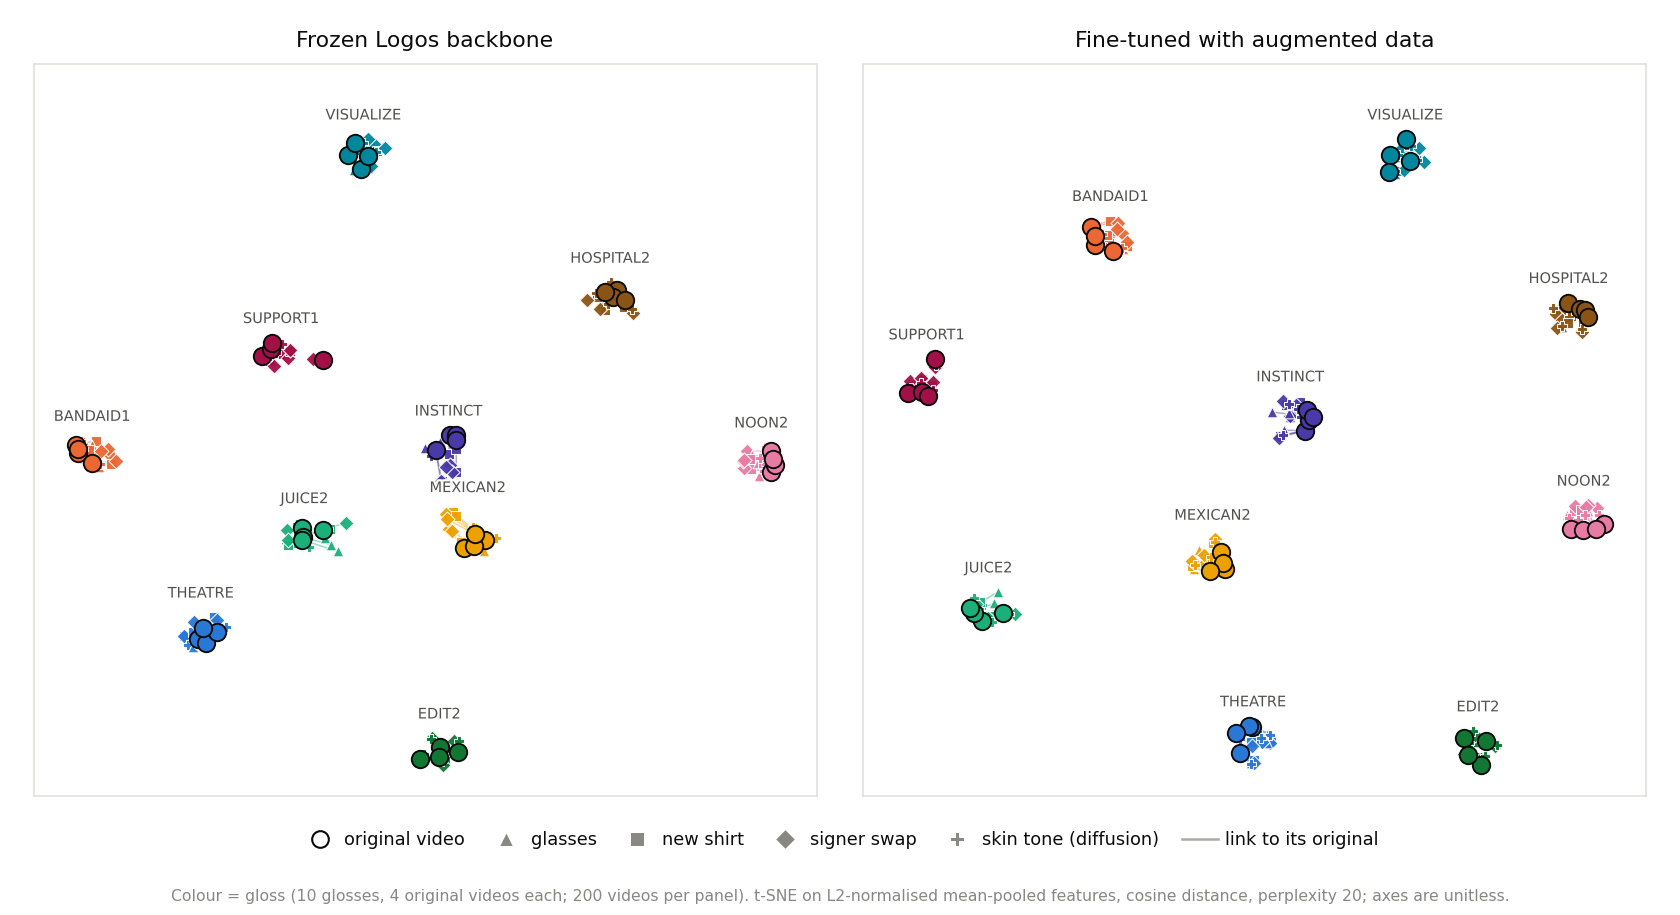
\includegraphics[width=.85\linewidth]{aug_vs_orig_tsne.png}
\caption[t-SNE of augmented copies vs.\ source videos]{t-SNE~\cite{vandermaatenVisualizingDataUsing2008} projection (cosine metric, perplexity 20, seed 0) of
$\ell_2$-normalised mean-pooled features for ten sampled glosses, four
original videos each, plus all four appearance-augmented copies per
original ($n{=}200$ per panel). Colour = gloss, marker = variant (large
outlined circles are originals), thin lines connect each copy to its
source. In the frozen space (left) and the aug-fine-tuned space (right),
augmented copies stay within their gloss cluster and near their source;
no variant-specific clusters emerge.}
\label{fig:aug_vs_orig_tsne}
\end{figure}

\begin{figure}[H]
\centering
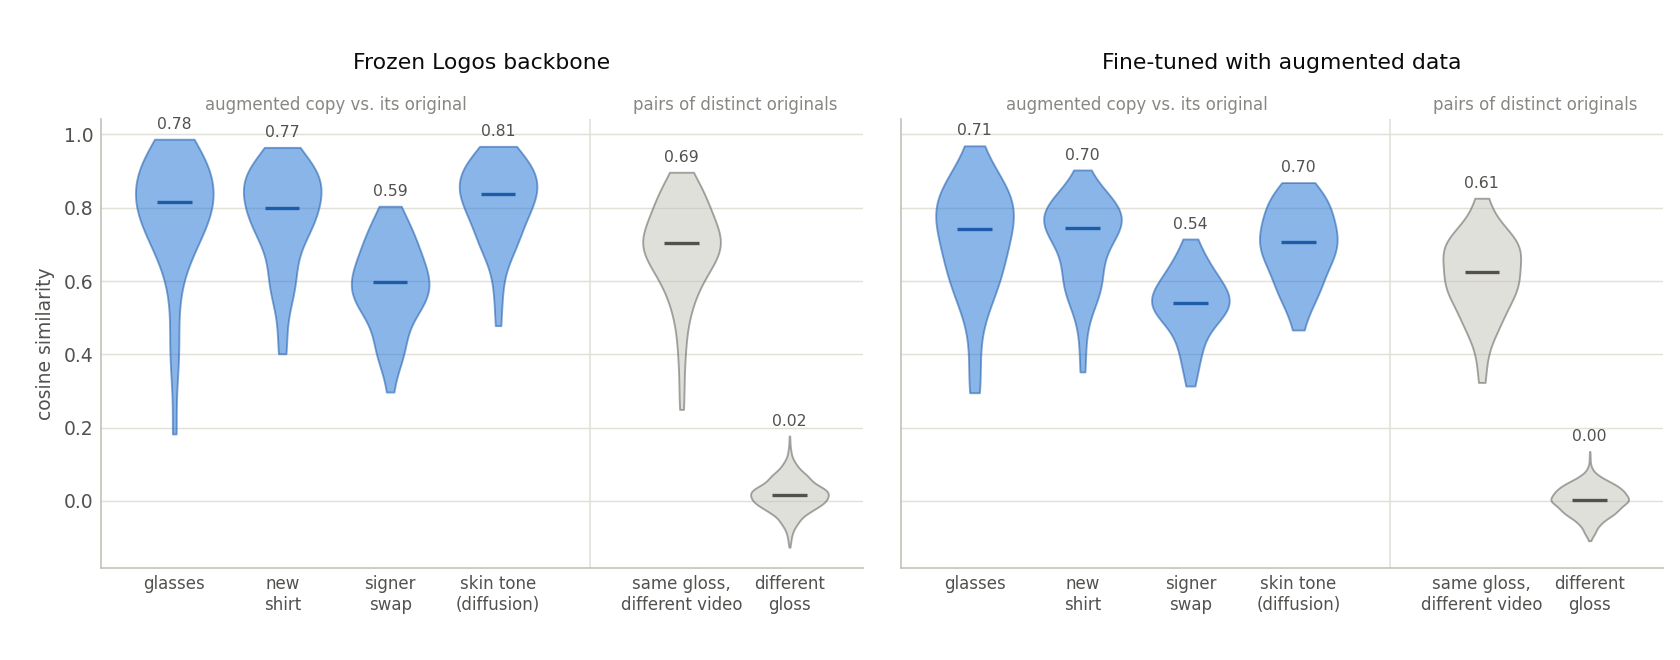
\includegraphics[width=.75\linewidth]{aug_vs_orig_cosine.png}
\caption[Cosine similarity of augmented copies to source]{Cosine similarity of each augmented copy to its source video,
per edit type, against two reference distributions from the same sample:
pairs of distinct same-gloss originals and different-gloss pairs. Local
edits (glasses, shirt, skin tone) sit above the same-gloss reference;
signer swap falls below it in both spaces.}
\label{fig:aug_vs_orig_cosine}
\end{figure}

\section{Generative appearance-edit prompts}
\label{app:flux_prompts}
The prompts used to generate the appearance counterfactuals of
\S\ref{sec:method-diffusion}, verbatim from the generation code. Shared
clauses are factored out as in the implementation, and each edit prompt
names the clauses it appends; braced placeholders are filled per video
from the vocabularies below.

\paragraph{Clause L (no extra limbs), appended to every prompt.}
\begin{quote}\small\itshape
Do NOT add, invent, duplicate, complete or remove any hand, arm or finger.
The output must contain exactly the same hands and arms, in exactly the
same positions, as this input frame --- and no others. If a hand or arm is
lowered, occluded, or outside the frame here, it MUST remain absent: never
raise or draw a hand that is not clearly visible in this input frame.
\end{quote}

\paragraph{Clause P (appearance preservation), used by the clothing and glasses edits.}
\begin{quote}\small\itshape
You MUST NOT change ANY of the following: the exact shape and position of
every finger and hand, wrist angles, arm positions and trajectory, facial
expression, eye gaze direction, mouth shape, body posture, skin tone,
hair, and the background. Only the clothing appearance changes. [Clause L]
\end{quote}

\paragraph{Clause G (geometry preservation), used by the skin-tone edit.}
\begin{quote}\small\itshape
You MUST NOT change ANY of the following: the exact shape and position of
every finger and hand, wrist angles, arm positions and trajectory, facial
expression, eye gaze direction, mouth shape, body posture, hair, clothing,
and the background. Keep the person's identity and all motion identical.
[Clause L]
\end{quote}

\paragraph{Clause M (motion and expression preservation), used by the signer swap.}
\begin{quote}\small\itshape
You MUST NOT change ANY of the following: the exact shape and position of
every finger and hand, wrist angles, both arms' positions and trajectory,
body posture, head pose, and the facial EXPRESSION --- eyebrow position,
eye openness, gaze direction and mouth shape, exactly as they appear in
this frame. Keep the background, camera framing and lighting unchanged.
[Clause L]
\end{quote}

\paragraph{Shirt.}
\begin{quote}\small\itshape
Edit this image: change the person's shirt or top to solid \{color\}.
[Clause P]
\end{quote}

\paragraph{Glasses.}
\begin{quote}\small\itshape
Edit this image: add a pair of thin-framed glasses on the person's face.
Do not change the clothing, hair, skin tone, or background. [Clause P]
\end{quote}

\paragraph{Skin tone.}
\begin{quote}\small\itshape
Edit this image: change ONLY the person's skin tone to a \{description\}
complexion (Monk skin tone tier \{tier\}, approx \{hex\}). Apply the same
tone naturally and consistently to the face, neck, arms and both hands,
matching the original lighting and shading. [Clause G]
\end{quote}

\paragraph{Signer swap.}
\begin{quote}\small\itshape
Edit this image: completely change the person's appearance so they look
like \{identity\}. Change their face shape and features, skin tone, hair,
apparent age, gender presentation and clothing to match that description.
[Clause M]
\end{quote}

\paragraph{Vocabularies.}
\emph{Shirt} colours: bright red, royal blue, forest green, deep purple,
bright orange, hot pink, navy blue, crimson, teal, golden yellow.
\emph{Skin-tone} tiers and their prompt wording are given in
Table~\ref{tab:mst_tiers}. The ten \emph{signer-swap} identities are: an
elderly Black woman in her 70s with
short grey natural hair and thin gold-rimmed glasses, wearing a plum
cardigan; a young East Asian man in his 20s with short straight black
hair, clean-shaven, wearing a plain charcoal t-shirt; a middle-aged South
Asian man with a full black beard, wearing a grey collared shirt; a young
white woman in her 20s with long blonde hair tied back, light freckles,
wearing a maroon sweater; a heavyset older white man in his 60s, bald with
a short grey beard, wearing a blue plaid flannel shirt; a Black man in his
30s with short cropped hair and a neatly trimmed beard, wearing a black
hoodie; a Latina woman in her 40s with shoulder-length wavy dark-brown
hair and gold hoop earrings, wearing a forest-green blouse; a
Middle-Eastern woman in her 30s wearing a navy headscarf and a
long-sleeved beige top; an older East Asian woman in her 60s with short
permed grey-black hair and rectangular glasses, wearing a lavender knit
cardigan; and a teenage boy with short curly dark hair and a faint
moustache, wearing a bright red crewneck sweatshirt.

\begin{table}[H]
\centering
\small
\begin{tabular}{ccl}
\toprule
\textbf{Tier} & \textbf{Reference} & \textbf{Prompt description} \\
\midrule
5  & \#d7bd96 & light tan \\
6  & \#a07e56 & tan brown \\
7  & \#825c43 & medium-dark brown \\
8  & \#604134 & dark brown \\
9  & \#3a312a & deep brown \\
10 & \#292420 & very deep ebony brown \\
\bottomrule
\end{tabular}
\caption[Monk skin tone tiers used by the skin-tone edit]{The six Monk
Skin Tone tiers used by the skin-tone edit, with the reference value and
the wording passed to the editor. Tiers $1$--$4$ are excluded: lighter
tones are already well represented among the corpus signers.}
\label{tab:mst_tiers}
\end{table}


\section{t-SNE projections of the embedding spaces}
\label{app:tsne_grid}
% FIGURE (t-SNE grid) redesigned 2026-07-30: the original 58-gloss probe
% set (built for the gendered-pair analogy task) turned up ZERO glosses
% sharing an exact 5/5 ASL-LEX phonological match among its high-iconicity
% members, so the gloss subset was replaced with 6 real phonological
% "minimal families" (triplets, exact match on MajorLocation/MinorLocation/
% Handshape/Movement/SignType) found by a full-corpus search over all 2725
% ASL-Citizen train glosses joined to ASL-LEX (994 rated; provenance:
% family_search_full.py, probe_families.json). Families were further
% chosen (2026-07-30 refinement) to MAXIMIZE diversity ACROSS families:
% MajorLocation/MinorLocation are Neutral for every eligible candidate (a
% hard property of this corpus, not a choice), so the 6 families instead
% cover 6 distinct handshapes (the max of 8 available given the 6-family
% cap) and jointly represent all 3 Movement values and both SignType
% values. Colour now encodes family, marker shape encodes
% member-within-family (consistent across all 9 panels). Panel set:
% dropped the two pair-SupCon panels (K=3, K=5);
% added the fine-tuned-feature SignCLIP family (augft_on_{ce,aug,sdda})
% and the headless fine-tuned-backbone "Logos" family (ce, aug) --
% extracted via dump_kq_spaces_families.py (cluster job 25054868, genoa
% CPU partition, no GPU/SBU cost). augft_on_sdda has no bare-backbone
% sibling in the grid (ce/aug were chosen over sdda/consistency as the
% two healthiest backbone-FT recipes per the signer-probe results above);
% this is a deliberate 9th-panel choice, not an oversight. The
% signer-coloured twin is still NOT buildable from local caches (kqfeat
% exports carry no signer or video IDs) and stays deferred to
% jobs/visualize_embedding_spaces.job.
\begin{figure*}[t]
\centering
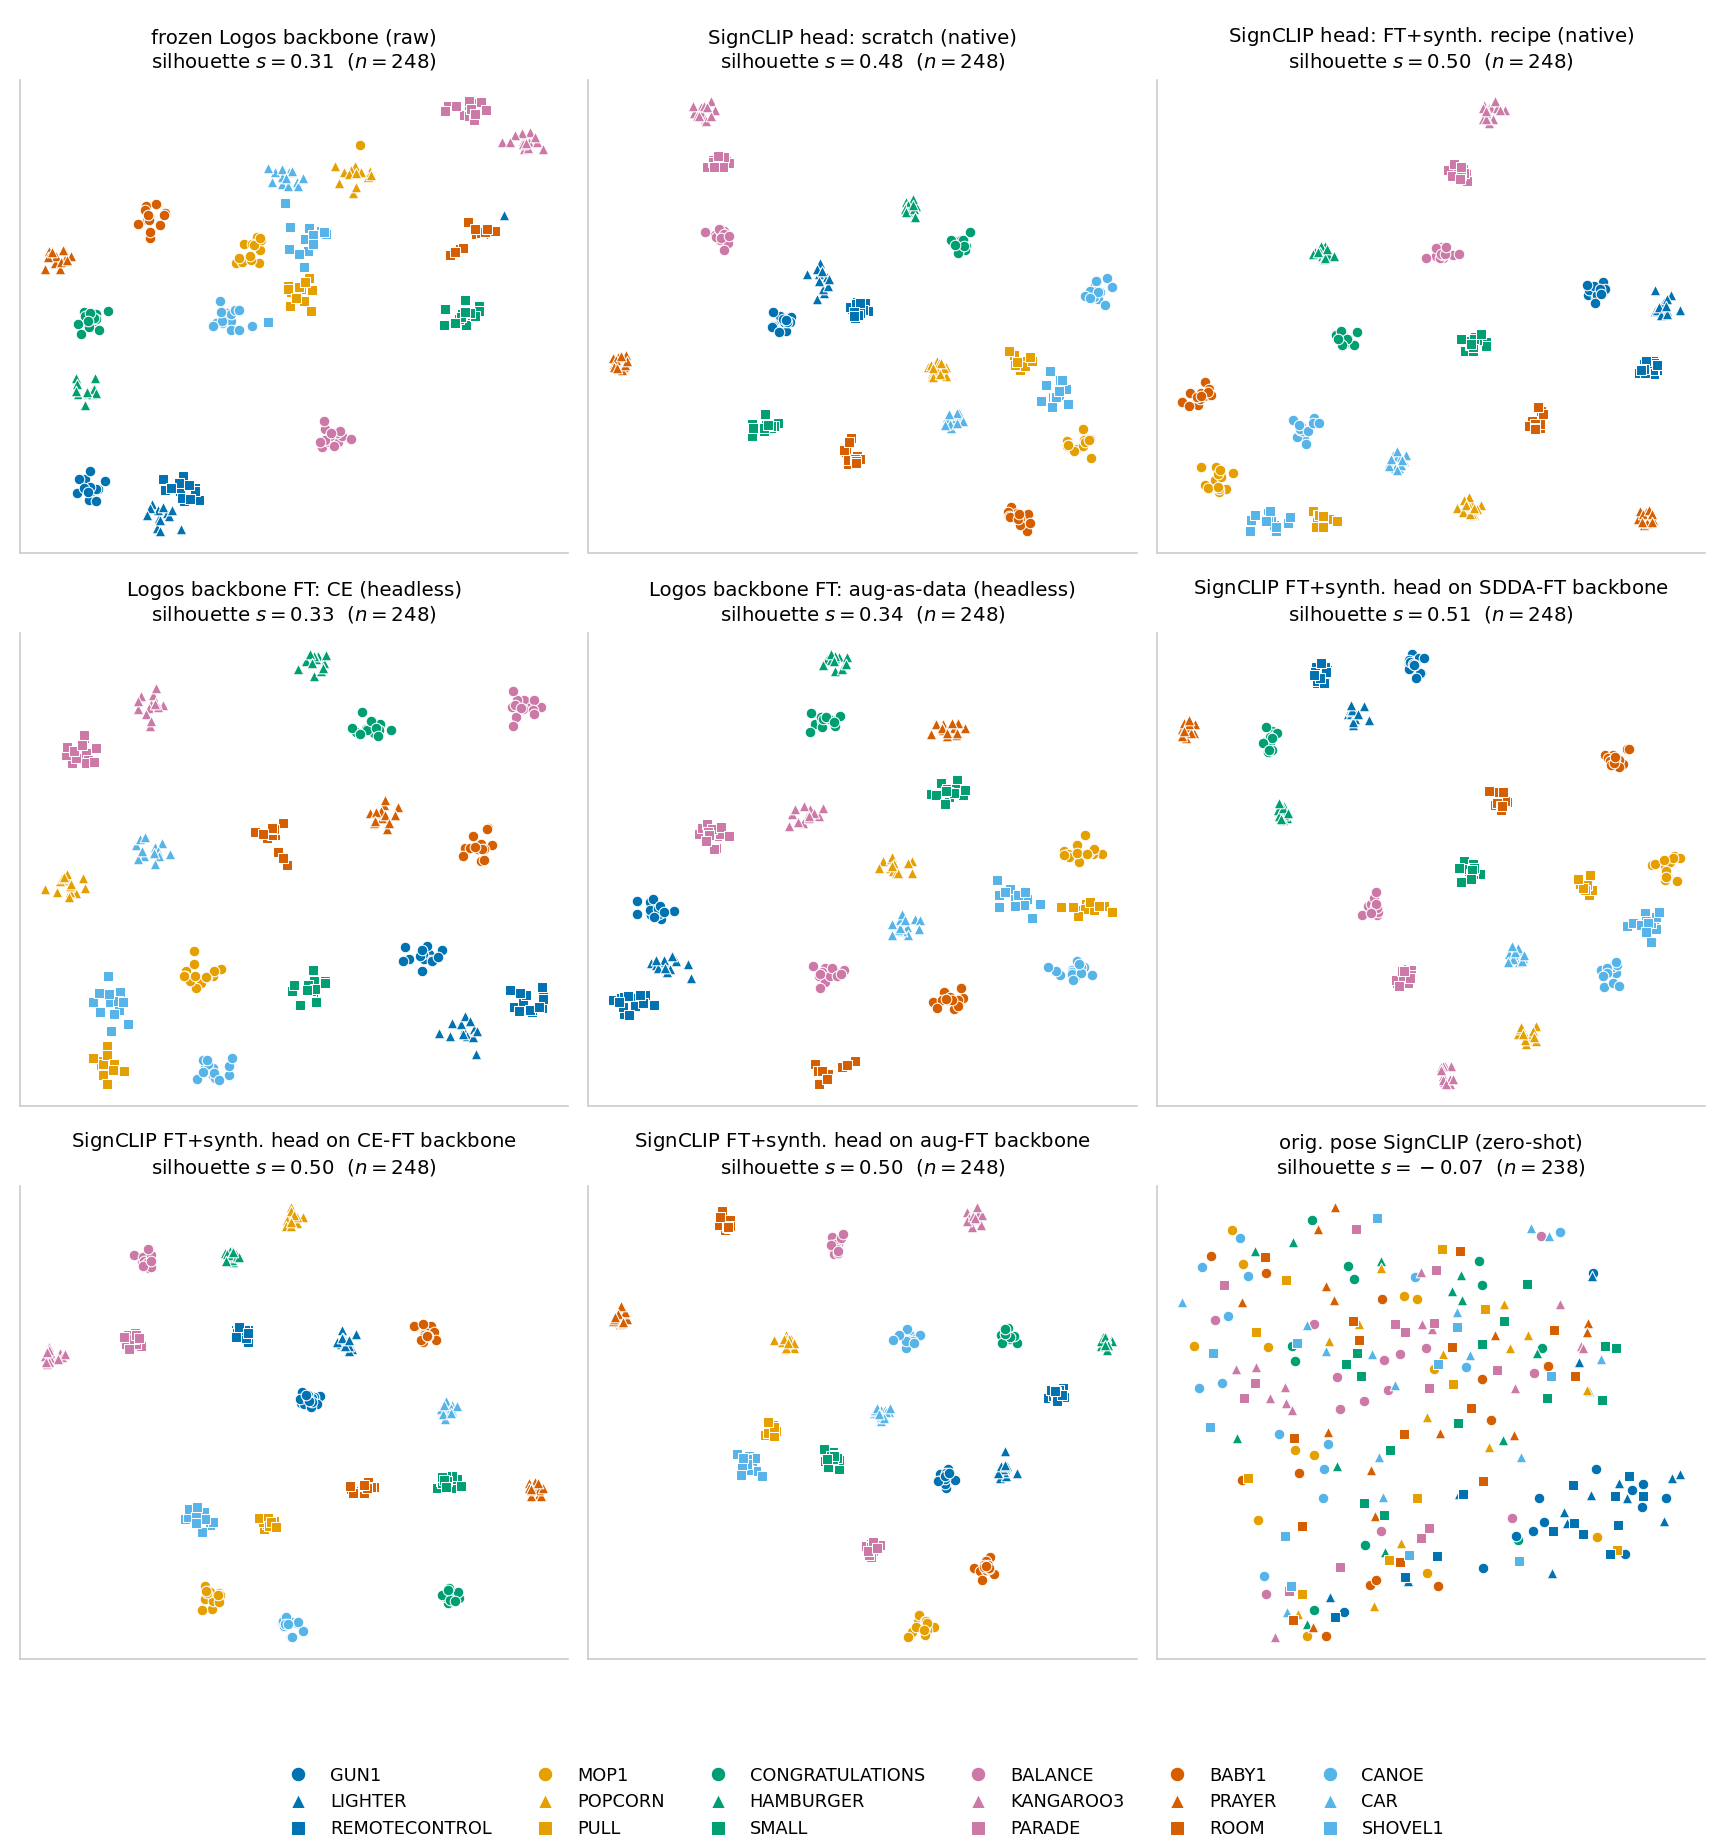
\includegraphics[width=.85\textwidth]{tsne_grid_gloss.png}
\caption[t-SNE projections across nine embedding spaces]{t-SNE projections (shared hyper-parameters: perplexity 30, PCA
initialisation, fixed seed) of the same video sample in nine embedding
spaces. The 18 plotted glosses are six phonological ``minimal families''
(triplets): groups of three ASL-Citizen glosses that are simultaneously
high-iconicity (top tertile of ASL-LEX deaf-signer ratings among
well-sampled train glosses), share an exact match on all five ASL-LEX
form features (major/minor location, handshape, movement, sign type), and
were chosen to be as phonologically distinct from one another as the
corpus allows -- major/minor location is Neutral for every eligible
family (unavoidable: that is where high-iconicity phonological overlap
concentrates in this corpus), but the six families span six different
handshapes and, jointly, all three movement types and both sign types --
e.g.\ \{CANOE, CAR, SHOVEL1\}, all Neutral-space, S handshape, curved,
symmetrical/alternating signs, versus \{GUN1, LIGHTER, REMOTECONTROL\},
Neutral-space but A handshape, no path movement, one-handed. Colour
identifies the family, marker shape the member within it, consistent
across every panel so the same gloss can be tracked across spaces ($n$
per panel in the title). Panel titles report the silhouette score $s$ of
the plotted clips computed in the original 768-dimensional L2-normalised
feature space, so cluster quality is a property of the space rather than
of the projection. Every Logos-based space separates these hard,
phonologically-confusable cases by gloss ($s{=}0.31$--$0.51$): the frozen
backbone alone is loosest ($s{=}0.31$), backbone fine-tuning helps a
little (CE $0.33$, aug $0.34$), and every SignCLIP head is tighter still,
with the three fine-tuned-feature heads (on CE/aug/SDDA-FT backbones,
$s{=}0.50$--$0.51$) essentially matching the frozen-backbone head
($s{=}0.50$). The original pose-based SignCLIP model (bottom right;
$n{=}238$ where pose extraction succeeds) shows no gloss structure on
this out-of-domain sample ($s{=}-0.07$). A signer-coloured companion
requires per-clip signer metadata not present in the cached exports and
is deferred to the embedding-visualisation job.}
\label{fig:tsne_grid}
\end{figure*}


\end{document}
